\documentclass{article}
\usepackage{xeCJK}
\defaultCJKfontfeatures{AutoFakeBold=true,AutoFakeSlant=true}
\setCJKmainfont{思源宋体}
\setCJKmonofont{思源等宽}
\setCJKsansfont{思源黑体}
\usepackage{NotesTeX}
\usepackage{multicol}
\usepackage{tabu}
\usepackage{pgfplots}
\usepackage{subcaption}
\usepackage{tasks}
\pgfplotsset{compat=newest}
\usetikzlibrary{calc,patterns,quotes,angles,intersections,arrows}
\usepgfplotslibrary{fillbetween}

\newenvironment{situation}{\paragraph{适用情形:}}{}
\newenvironment{solution}{\paragraph{Solution.}}{}
\tcolorboxenvironment{situation}{
    boxrule=0pt,
    boxsep=0pt,
    colback={White!90!Green},
    enhanced jigsaw,
    borderline west={2pt}{0pt}{Green},
    sharp corners,
    before skip=10pt,
    after skip=10pt,
    breakable,
}
\tcolorboxenvironment{solution}{
    boxrule=0pt,
    boxsep=0pt,
    blanker,
    borderline west={2pt}{0pt}{NavyBlue!80!white},
    before skip=10pt,
    after skip=10pt,
    left=12pt,
    right=12pt,
    breakable,
}

\newcommand*\diff{\mathop{}\!\mathrm{d}}

\title{
    {\Huge 数学笔记}\\
    {\large{\textit{一些关于解题方法的总结}}}
}
\author{L.Sun}
\emailAdd{zover.v@gmail.com}

\begin{document}
\maketitle
\pagestyle{fancynotes}

% \part{极限、连续}

\section{求数列极限}
数列极限的求解一般常用单调有界法、两边夹法、列紧性定理和柯西准则等等。下面对这几种常用方法进行总结。
\subsection{\texorpdfstring{$ \delta - \varepsilon  $}{δ-ε} 语言证明}
当需要证明$\lim_{n \to \infty} a_n = A$时,可以通过证明不等式$ \left\lvert a_n - A\right\rvert < \varepsilon $成立。
\begin{situation}
    适用于给出数列递推公式的情况
\end{situation}
\paragraph{方法一} 直接对不等式证明:
\begin{proof}
    \[
        \forall \varepsilon > 0, ~ \exists N ~ \text{s.t. when}~ n > N,~
        \left\lvert a_n - A\right\rvert < \varepsilon
    \]
\end{proof}


\paragraph{方法二} 对不等式进行缩放间接证明:
\begin{proof}
    由\[ \left\lvert a_n - A \right\rvert \leq \varphi(n) < \varepsilon \]
    得出 \[ n > \psi(\varepsilon) \]
    不妨令 $N = \psi(\varepsilon)$,所以当 $n > N$时,恒有
    \[ \left\lvert a_n - A\right\rvert < \varepsilon \]
    $\lim_{n \to \infty} a_n$存在
\end{proof}

\begin{example}
    设$ a > 1 $,证明$ \lim_{n \to \infty} \sqrt[n]{a} = 1 $
\end{example}
\begin{proof}
    根据几何不等式,得
    \[
        \left\lvert \sqrt[n]{a} - 1 \right\rvert
        = \sqrt[n]{a} - 1
        = (a \cdot \underbrace{1\cdots1}_{n-1})^{1/n} - 1
        < \frac{a+(n-1)}{n} - 1
        = \frac{a-1}{n}
    \]
    令$ \frac{a-1}{n}<\varepsilon $,即$ n > \frac{a-1}{\varepsilon} $。
    不妨令$N = \frac{a-1}{\varepsilon}$,则有
    \[
        \forall\varepsilon>0 \text{ and } n > N \qquad \left\lvert \sqrt[n]{a}-1 \right\rvert<\varepsilon
    \]
    所以$\lim_{n \to \infty} = 1$成立。
\end{proof}

\pagebreak
\subsection{单调有界法则}
单调有界法通常找出数列的上界(下界)。证明在趋于无穷时,数列单调增(单调减)。若有递推式,直接将递推式中的数列项换为极限值(未知数)进行求解。
\begin{theorem}
    \label{th:单调有界法则}
    单调有界数列必有极限
\end{theorem}
\begin{situation}
    适用于给出数列递推公式地情况
\end{situation}
\begin{example}
    设$a>0, x_1 > 0, x_{n+1} = \frac{1}{2}(x_n+\frac{a}{x_n}) (n=1,2,\cdots)$,求$lim_{n\to\infty}x_n$
\end{example}
\begin{proof}
    由于
    \begin{alignat*}{2}
        x_{n+1}         & = \frac{1}{2}(x_n+\frac{a}{x_n}) & \geq  \sqrt{a} \\
        x_{n} - x_{n+1} & = \frac{1}{2x_n}(x_n^2-a)        & \geq  0
    \end{alignat*}
    所以$\{x_n\}$为单调有界数列,故可设$lim_{n\to\infty} x_n = A$,当$n\to\infty$时,关系式
    \[ x_{n+1} = \frac{1}{2}(x_n+\frac{a}{x_n}) \]
    变为
    \[ A = \frac{1}{2}(A+\frac{a}{A}) \]
    解得$A=\sqrt{a}$,故$lim_{n\to\infty}=\sqrt{a}$
\end{proof}

\subsection{两边夹法则}
两边夹法则通常将数列左右两侧进行合适地缩放,两侧缩放得到地数列同时趋向同一个值时,则可以证明其极限存在。
\begin{theorem}
    \label{th:两边夹法则}
    (两边夹法则)若$n\to\infty$时,恒有
    \[ A \leftarrow x_n \leq y_n \leq z_n \implies A \]
    或$\forall \varepsilon > 0, n\to\infty$
    \[ A -\varepsilon \leftarrow x_n(\varepsilon) \leq y_n \leq z_n(\varepsilon) \implies A + \varepsilon \]
    则$\lim_{n \to\infty}=A$
\end{theorem}
\begin{situation}
    已知数列通项
\end{situation}
\begin{example}
    证明$\lim_{n\to\infty}\sqrt[n]{n} = 1$
\end{example}
\begin{proof}
    根据平均不等式\ref{eq:平均不等式},有
    \[ 1 \leq \sqrt[n]{n} = (\underbrace{1\cdot 1\cdots 1}_{n-2}\sqrt{n}\cdot\sqrt{n})^{1/n}\leq \frac{n-2+2\sqrt{n}}{n} < 1+\frac{2}{\sqrt{n}} \to 1 \]
    由两边夹法则可知,$\lim_{n\to\infty}\sqrt[n]{n} = 1$
\end{proof}

\pagebreak
\subsection{柯西准则}
在极限值未知地情况下,判断数列极限的存在性可用柯西准则。
\begin{theorem}
    \label{th:柯西准则}
    (柯西准则)数列$\{x_n\}$收敛$\iff  \forall\varepsilon>0,\exists N,\text{ s.t. }m,n>N, \lvert x_m-x_n\rvert<\varepsilon$
\end{theorem}
\begin{situation}
    只需判断极限是否存在
\end{situation}
\begin{example}
    证明数列$S_n=\sum_{k=1}^n \frac{1}{k}$发散
\end{example}
\begin{proof}
    因为
    \[ S_{2n} - S_{n} = \frac{1}{n+1}+\frac{1}{n+2}+\cdots+\frac{1}{n+n} \geq \frac{n}{2n} = \frac{1}{2}\]
    故${S_n}$发散。
\end{proof}

\subsection{运算法则}
如果数列由其它数列构成,且这些数列收敛,则可以通过运算法则,求出数列极限。
\begin{theorem}
    \label{th:数列极限运算法则}
    (运算性)设$\lim_{n\to\infty}x_n=A,\lim_{n\to\infty}y_n=B$,则有
    \begin{enumerate}
        \item $\lim_{n\to\infty} (x_n\pm y_n)=A\pm B$
        \item $\lim_{n\to\infty} x_ny_n=AB$
        \item $\lim_{n\to\infty} \frac{x_n}{y_n} = \frac{A}{B} \qquad (B\neq 0)$
    \end{enumerate}
\end{theorem}
\begin{situation}
    式子中含有收敛数列的组合(或者经过适当变形后),则可以通过运算法则求出极限
\end{situation}
\begin{example}
    求极限$\lim_{n\to\infty}\sqrt{n}(\sqrt{n-1}-\sqrt{n})$
\end{example}
\begin{solution}
    由于$\sqrt{n}$不存在,故不能直接用乘法法则,先经过适当变形
    \[
        \lim_{n\to\infty}   \sqrt{n}(\sqrt{n-1}-\sqrt{n})
        = \lim_{n\to\infty} \frac{\sqrt{n}}{\sqrt{n-1}+\sqrt{n}}
        = \lim_{n\to\infty} \frac{1}{1+\sqrt{1+\frac{1}{n}}}
        =\frac{1}{2}
    \]
\end{solution}

\begin{theorem}
    \label{th:数列极限保号性}
    (保号性)
    \[
        \text{If } \lim_{n\to\infty} x_n = A, \lim_{n\to\infty} y_n = B, A>B,
        \text{ s.t. } \exists N, n > N, x_n > y_n
    \]
\end{theorem}
\begin{theorem}
    \label{th:数列极限单调性}
    (单调性)
    \[
        \text{Let } \lim_{n\to\infty} x_n = A, \lim_{n\to\infty} y_n = B,
        \text{ if } x_n \geq y_n \text{ when } n\to\infty
        \text{ Hence } A \geq B
    \]
\end{theorem}
\begin{theorem}
    \label{th:数列极限子列性}
    (子列性)
    \[
        \lim_{n\to\infty} x_n = A \iff \lim_{n\to\infty} x_{k_n} = A \text{ for all sub array } \{x_{k_n}\} \text{ of } \{x_n\}
    \]
\end{theorem}

\subsection{Stolz定理}
类似与函数极限中的洛必达法则
\begin{theorem}
    \label{th:Stolz定理}
    若$\{y_n\}$\textcolor{red}{严格增无穷大},且有
    \[ \lim_{n\to\infty}\frac{x_n - x_{n-1}}{y_n - y_{n-1}} = A \]
    则有
    \[ \lim_{n\to\infty}\frac{x_n}{y_n} = A \]
\end{theorem}
\begin{situation}
    ~
    \begin{enumerate}
        \item 当数列通项中出现连加、连乘(指数对数化$x = \mathrm{e}^{\ln x}$将连乘转为连加)
        \item 当出现加减法的递推公式(即求\textcolor{red}{商差}的极限)时,可将问题转换为求解\textcolor{red}{商}的极限
    \end{enumerate}
\end{situation}
\begin{example}
    设$a_n>0 (n = 1, 2, \ldots) \lim_{n\to\infty}a_n = a$,证明$\lim_{n\to\infty}\sqrt[n]{a_1a_2\cdots a_n}=a$
\end{example}
\begin{proof}
    \[
        \lim_{n\to\infty} \sqrt[n]{a_1a_2\cdots a_n}
        =\exp(\lim_{n\to\infty}\frac{\ln a_1 + \cdots \ln a_n}{n})
        =\exp(\lim_{n\to\infty}\ln a_n) = \mathrm{e}^{\ln a} = a
    \]
\end{proof}
\begin{example}
    设$\lim_{n\to\infty}(x_n - x_{n-2}) = 0$,证明$\lim_{n\to\infty}\frac{x_n - x_{n-1}}{n} = 0$
\end{example}
\begin{proof}
    由于
    \[ \lim_{n\to\infty}\frac{x_{2n}}{2n} = \lim_{n\to\infty}\frac{x_{2n}-x_{2n-2}}{2n-(2n-2)} = 0 \]
    \[ \lim_{n\to\infty}\frac{x_{2n+1}}{2n+1} = \lim_{n\to\infty}\frac{x_{2n+1}-x_{2n-1}}{(2n+1)-(2n-1)} = 0 \]
    所以$\lim_{n\to\infty} \frac{x_n}{n} = 0$,从而
    \[ \lim_{n\to\infty}\frac{x_n - x_{n-1}}{n} = \lim_{n\to\infty}\frac{x_n}{n} - \lim_{n\to\infty}\frac{x_{n-1}}{n} = 0 \]
\end{proof}

\subsection{求和极限转积分}
根据积分的定义可以很容易知道如下公式
\[
    \int_{a}^{b} f(x) \,\diff x = (b-a)\lim_{n\to\infty}\frac{f(x_1) + f(x_2)+\cdots+f(x_n)}{n}\qquad x_i\in[a,b]
\]
此公式也可看做是$n$次蒙特卡洛积分后平均,其密度概率函数为$f_X(x)=\dfrac{1}{b-a}$
\[
    \int_a^b f(x) \,\diff x = \frac{1}{n}\sum_{i=1}^n \frac{f(x_i)}{\left.1\middle/(b-a)\right.}
\]
题目常常会出现求和极限的求解,此时可对原式变形后用积分求解。下式为常出现的情况:
\[
    \lim_{n\to\infty}\frac{1}{n}\left[f(\frac{1}{n}) + f(\frac{2}{n}) + \cdots + f(\frac{n}{n})\right] = \int_0^1 f(x) \,\diff x
\]


\section{函数极限}
\subsection{函数极限的概念}
由数列的极限类比,能得出如下定义
\begin{definition}
    \[ \lim_{x\to+\infty} f(x) = A \iff \forall\varepsilon >0, \exists X, \text{ 当~} x > X\text{ 时~}, \left\lvert f(x) - A \right\rvert < \varepsilon \]
    \[ \lim_{x\to-\infty} f(x) = A \iff \forall\varepsilon >0, \exists X, \text{ 当~} x < X\text{ 时~}, \left\lvert f(x) - A \right\rvert < \varepsilon \]
    \[ \lim_{x\to\infty}  f(x) = A \iff \forall\varepsilon >0, \exists X, \text{ 当~} \lvert x \rvert > X\text{ 时~}, \left\lvert f(x) - A \right\rvert < \varepsilon \]

    \[ \lim_{x\to x_0^+} f(x) = A \iff \forall\varepsilon > 0, \exists \delta > 0, \text{ 当~} 0 < x - x_0 < \delta \text{ 时~}, \left\lvert f(x) - A \right\rvert < \varepsilon \]
    \[ \lim_{x\to x_0^-} f(x) = A \iff \forall\varepsilon > 0, \exists \delta > 0, \text{ 当~} 0 < x_0 - x < \delta \text{ 时~}, \left\lvert f(x) - A \right\rvert < \varepsilon \]
    \[ \lim_{x\to x_0}   f(x) = A \iff \forall\varepsilon > 0, \exists \delta > 0, \text{ 当~} 0 < \lvert x-x_0 \rvert < \delta \text{ 时~}, \left\lvert f(x) - A \right\rvert < \varepsilon \]

    \[  \lim_{x\to x_0}  f(x) = A \iff \lim_{n\to x_0^-} f(x) = \lim_{n\to x_0^+} f(x) = A \]

    \[ \lim_{x\to x_0} f(x) = \infty \iff \forall M, \exists \delta > 0, \text{ 使得~} 0 < \lvert x-x_0 \rvert < \delta \implies \left\lvert f(x) \right\rvert > M \]
    \[ \lim_{x\to x_0} f(x) = +\infty \iff \forall M, \exists \delta > 0, \text{ 使得~} 0 < \lvert x-x_0 \rvert < \delta \implies f(x) > M \]
    \[ \lim_{x\to x_0} f(x) = -\infty \iff \forall M, \exists \delta > 0, \text{ 使得~} 0 < \lvert x-x_0 \rvert < \delta \implies f(x) < M \]
\end{definition}

\subsection{与数列极限的相似之处}
\begin{enumerate}
    \item 利用$\varepsilon-\delta$方式解函数的极限与数列的极限同理
    \item 运算法则相同
          \sidenote{
              对于有理函数$Q(x)$,即
              \[ Q(x) = \frac{a_0 + a_1x + \cdots + a_nx^n}{b_0 + b_1x + \cdots + b_mx^m} \]
              其中$a \neq 0, b \neq 0$,则有
              \begin{equation*}
                  \lim_{x\to\infty}Q(x) =
                  \begin{cases}
                      \frac{a_n}{b_m} & n=m \\
                      0               & n<m \\
                      \infty          & n>m
                  \end{cases}
              \end{equation*}
          }
    \item 局部保号性(\ref{th:数列极限保号性})
    \item 局部单调性(\ref{th:数列极限单调性})
    \item 两边夹法则(\ref{th:两边夹法则})
\end{enumerate}

\subsection{海涅定理}
当研究函数极限时,可以将函数转为数列进行极限的求解。
\begin{theorem}
    (海涅定理)
    \label{th:海涅定理}
    \[ \lim_{x\to x_0}f(x) = A \iff \forall x_n \to, \neq x_0, \text{ 都有~} \lim_{n\to\infty}f(x_n) = A \]
\end{theorem}
\begin{situation}
    证明极限不存在时,可以将函数$f(x)$转为研究$f(a_n)$和$f(b_n)$的极限,
    利用极限的唯一性可知,
    \begin{equation*}
        \lim_{x\to x_0}f(x) =
        \begin{cases}
            A             & \lim_{n\to\infty}f(a_n) = \lim_{n\to\infty}f(b_n) = A \\
            \text{不存在} & \lim_{n\to\infty}f(a_n) \neq \lim_{n\to\infty}f(b_n)
        \end{cases}
    \end{equation*}
\end{situation}
\begin{example}
    证明$\lim_{x\to 0}\sin\frac{1}{x}$不存在
\end{example}
\begin{proof}
    取$x_n=1/(2n\pi), y_n=1/(2n\pi + \pi/2)$则有
    \[ \lim_{n\to\infty}f(x_n) = 0 \neq 1 = \lim_{n\to\infty}f(y_n) \]
    根据海涅定理,$\lim_{x\to 0}\sin\frac{1}{x}$不存在。
\end{proof}

\subsection{变量代换(复合函数极限)}
当求解复合函数的极限时,外层函数极限转为内层函数极限。
\begin{theorem}
    \label{th:变量代换法则}
    (变量代换法则)
    \begin{enumerate}
        \item (去心法则)$\text{若~} x \to x_0\text{ 时~}, g(x)\to,\neq y_0, \text{ 则~}\lim_{y\to y_0}f(y)=A\text{ 时,}$
              \[ \lim_{x\to x_0} f(g(x)) = \lim_{y\to y_0} f(y) = A \]
        \item (连续法则)$\text{若~} \lim_{x\to x_0} g(x) = y_0 \text{ 且~} \lim_{y\to y_0} f(y) = f(y_0), \text{ 则,}$
              \[ \lim_{x\to x_0} f(g(x)) = f(\lim_{x\to x_0} g(x)) = f(y_0) \]
    \end{enumerate}
    注:去心和连续指的是$f(y)$在$y_0$处的连续性。
\end{theorem}

\subsection{等价公式}
等价公式在求解极限时,能很好地减少极限化简的计算量。
\begin{theorem}
    \label{th:等价公式}
    $\text{设~}x\to x_0\text{ 时~},\omega(x)\to,\neq 0, \text{则~}x\to x_0\text{ 时, 必有}$
    \begin{multicols}{2}
        \begin{enumerate}
            \item $\sin \omega(x) \sim \omega(x)$
            \item $\tan \omega(x) \sim \omega(x)$
            \item $\ln (1+\omega(x)) \sim \omega(x)$
            \item $\mathrm{e}^{\omega(x)}-1 \sim \omega(x)$
            \item $(1+\omega(x))^\alpha -1 \sim \alpha \omega(x) \qquad (\alpha \neq 0)$

            \item $1-\cos \omega(x) \sim \frac{1}{2}\omega^2(x)$
            \item $\omega(x)-\ln(1+\omega(x)) \sim \frac{1}{2}\omega^2(x)$
            \item $\mathrm{e}^{\omega(x)}-1-\omega(x) \sim \frac{1}{2}\omega^2(x)$

            \item $\tan \omega(x)-\omega(x) \sim \frac{1}{3}\omega^3(x)$
            \item $\omega(x)-\arctan \omega(x) \sim \frac{1}{3}\omega^3(x)$

            \item $\omega(x)-\sin \omega(x) \sim \frac{1}{6}\omega^3(x)$
            \item $\arcsin \omega(x) - \omega(x) \sim \frac{1}{6}\omega^3(x)$
            \item $\frac{\pi}{2} - \arccos \omega(x) - \omega(x) \sim \frac{1}{6}\omega^3(x)$

        \end{enumerate}
    \end{multicols}
\end{theorem}
\begin{situation}
    等价公式替换一般用于极限的\textcolor{red}{乘除过程}中。
    对于加减的极限,根据运算法则,\textcolor{red}{加减项必须的极限必须存在},才能进行替换(题中一般不会出现这种情况)。
    在使用等价公式时,通过对极限式子进行乘除调整,让其能消除某些项,从而达到简化的目的。


    \textbf{注:}此法本质时利用泰勒展开的第一项(一阶导数)进行计算,对于加减时,容易被消掉,故而对于加减的情况一般将其转为乘除形式。
\end{situation}

\begin{example}
    求极限$\lim_{x\to 0}\frac{1}{x^3}\left[ \left( \frac{2+\cos x}{3} \right)^x -1 \right] $
\end{example}
\begin{solution}
    \begin{align*}
          & \lim_{x\to 0}\frac{1}{x^3}\left[ \left( \frac{2+\cos x}{3} \right)^x -1 \right]    &                                                                 \\
        = & \lim_{x\to 0} \frac{1}{x^3}\left( \mathrm{e}^{x\ln\dfrac{2+\cos x}{3}} - 1 \right) & \qquad\text{替换~} \mathrm{e}^{\omega(x)}-1 \sim \omega(x)      \\
        = & \lim_{x\to 0} \frac{1}{x^3}\left( x\ln\dfrac{2+\cos x}{3} \right)                  &                                                                 \\
        = & \lim_{x\to 0} \frac{1}{x^2}\left[ \ln(1 + \dfrac{\cos x -1}{3})\right]             & \qquad\text{替换~} \ln(1+\omega(x)) \sim \omega(x)              \\
        = & \lim_{x\to 0} \frac{1}{x^2}\left( \dfrac{\cos x -1}{3} \right )                    & \qquad\text{替换~} 1-\cos \omega(x) \sim \frac{1}{2}\omega^2(x) \\
        = & \lim_{x\to 0} \frac{1}{x^2}\left( -\frac{1}{6}x^2 \right)                          &                                                                 \\
        = & -\frac{1}{6}
    \end{align*}
\end{solution}

\subsection{洛必达法则}
洛必达法则可以将用代入方法计算的极限转化为导数商的极限,从而解决复杂的极限计算。
\begin{theorem}
    \label{th:洛必达法则}
    (洛必达法则)
    ~
    \begin{enumerate}
        \item $\text{设~}x\to x_0\text{ 时}, f(x),g(x)\text{ 是无穷小且~}g'(x)\neq 0,$
        \item $\text{设~}x\to x_0\text{ 时}, g(x)\text{ 是无穷大且~}g'(x)\neq 0,$
    \end{enumerate}
    \[ \text{若~}\lim_{x\to x_0}\frac{f'(x)}{g'(x)}=A, \text{ 则~} \lim_{x\to x_0}\frac{f(x)}{g(x)}=A \]
\end{theorem}
\begin{situation}
    在使用洛必达法则时,应尽量先尝试直接代入计算,再用等价公式进行变形化简,最后才使用洛必达,这样能减少不必要的求导计算。
\end{situation}
\begin{example}
    $\text{设~}y=\left(\frac{\pi}{2}-\arctan x\right)^{\frac{1}{\ln x}}, \text{ 求~}\lim_{x\to +\infty}y$
\end{example}
\begin{solution}
    \begin{align*}
        \lim_{x\to +\infty}\ln y
         & = \lim_{x\to +\infty}\frac{\ln\left(\frac{\pi}{2}-\arctan x\right)}{\ln x}                                     \\
         & = \lim_{x\to +\infty}\left. \frac{-1}{(1+x^2)\left(\frac{\pi}{2}-\arctan x\right)} \middle/ \frac{1}{x}\right. \\
         & = \lim_{x\to +\infty} \frac{-1/x}{\frac{\pi}{2}-\arctan x}                                                     \\
         & = \lim_{x\to +\infty} \frac{1/x^2}{-\frac{1}{1+x^2}} = -\lim_{x\to +\infty} \left(1+\frac{1}{x^2}\right)       \\
         & =-1
    \end{align*}
    所以 $\lim_{x\to +\infty}y=\mathrm{e}^{-1}$
\end{solution}

\subsection{泰勒公式}
泰勒公式求极限属于万金油的方法。
\begin{theorem}
    \label{th:泰勒公式}
    (泰勒公式)
    设函数$f(x)$在$x_0$点的邻域$(a,b)$内有$n+1$阶导数,则对$\forall x\in (a,b)$,都有介于$x_0$和$x$之间的$\xi$,使得
    \begin{multline*}
        f(x) = f(x_0) + f'(x_0)(x-x_0) + \frac{f''(x_0)}{2!}(x-x_0)^2+\cdots\\
        +\frac{f^{(n)}(x_0)}{n!}(x-x_0)^n+\frac{f^{n+1}(\xi)}{(n+1)!}(x-x_0)^{n+1}
    \end{multline*}
\end{theorem}
\begin{situation}
    对极限中的复杂项展开至相同阶数,化简后进行求解
\end{situation}
\begin{example}
    求\[ \lim_{x\to +\infty}\left[x-x^2\ln\left(1+\frac{1}{x}\right)\right] \]
\end{example}
\begin{solution}
    \[
        \lim_{x\to +\infty}\left[x-x^2\ln\left(1+\frac{1}{x}\right)\right]
        = \lim_{x\to +\infty}\left[x-x^2\left(\frac{1}{x}-\frac{1}{2x^2}\right)\right]
        = \lim_{x\to +\infty}(x-x+\frac{1}{2})
        =\frac{1}{2}
    \]
\end{solution}

\section{函数的连续性}
\subsection{连续性}
函数的连续性考察,常常出现于选择题中。故对函数连续的基本概念要牢牢掌握。
\begin{definition}
    (连续性)
    \begin{alignat*}{4}
         & \lim_{x\to x_0^-}f(x) & ~ = f(x_0) & = \lim_{x\to x_0^+}f(x) & \text{ (连续)}   \\
         & \lim_{x\to x_0^-}f(x) & ~ = f(x_0) &                         & \text{ (左连续)} \\
         &                       & ~ f(x_0)   & = \lim_{x\to x_0^+}f(x) & \text{ (右连续)}
    \end{alignat*}
    当任何一项不存在或等号不成立时,则函数在$x_0$不连续(左不连续、右不连续)。
\end{definition}

\begin{theorem}
    \label{th:连续函数运算性}
    (运算性)
    设函数$f(x),g(x)$在$x_0$处连续,则函数$f(x)\pm g(x), f(x)g(x), \frac{f(x)}{g(x)} (g(x)\neq 0)$在$x_0$处连续
    \\
    若$g(u)$在$u=f(x_0)$处连续,则复合函数$g\circ f(x)$在$x_0$处连续
\end{theorem}

\subsection{间断点}
当讨论函数的间断点时,具体步骤如下:
\begin{enumerate}
    \item 考虑其定义域,找到其间断点
    \item 计算间断点的左右极限,(间断点可能有定义)
    \item 根据间断点的左右极限,判断间断点的类型
\end{enumerate}
\begin{marginfigure}
    \centering
    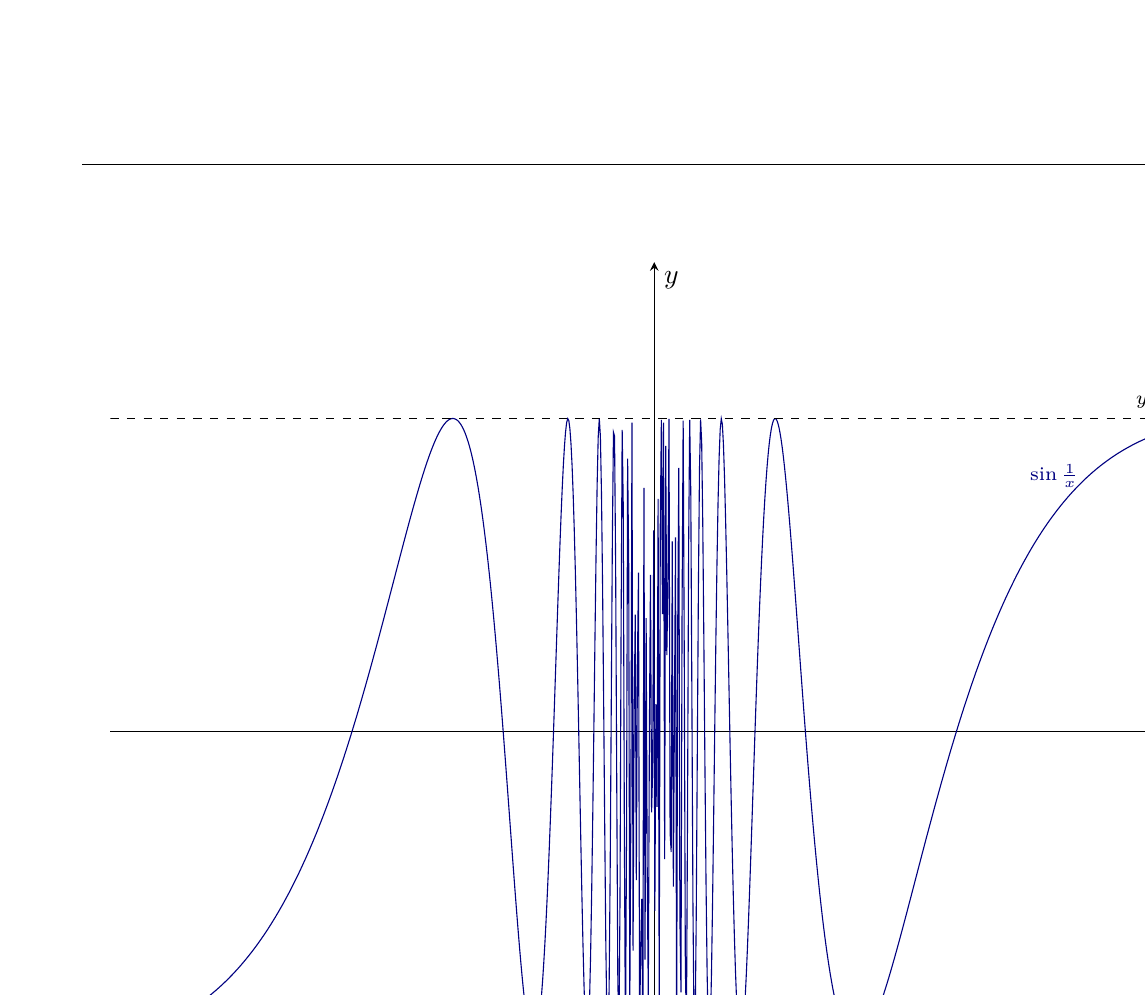
\begin{tikzpicture}
        \begin{axis}[
                ticks=none,
                axis lines=middle,
                ymin=-1.5,
                ymax=1.5,
                domain=-0.01:0.01,
                xlabel=$x$,
                ylabel=$y$,
                scale only axis,
                width=\textwidth
            ]
            \addplot[NavyBlue,samples=1000] {sin(1/x)} node[pos=0.998,left]{\scriptsize$\sin\frac{1}{x}$};
            \addplot[dashed]{1}  node[above left]{\scriptsize$y=1$};
            \addplot[dashed]{-1} node[below left]{\scriptsize$y=-1$};
        \end{axis}
    \end{tikzpicture}
    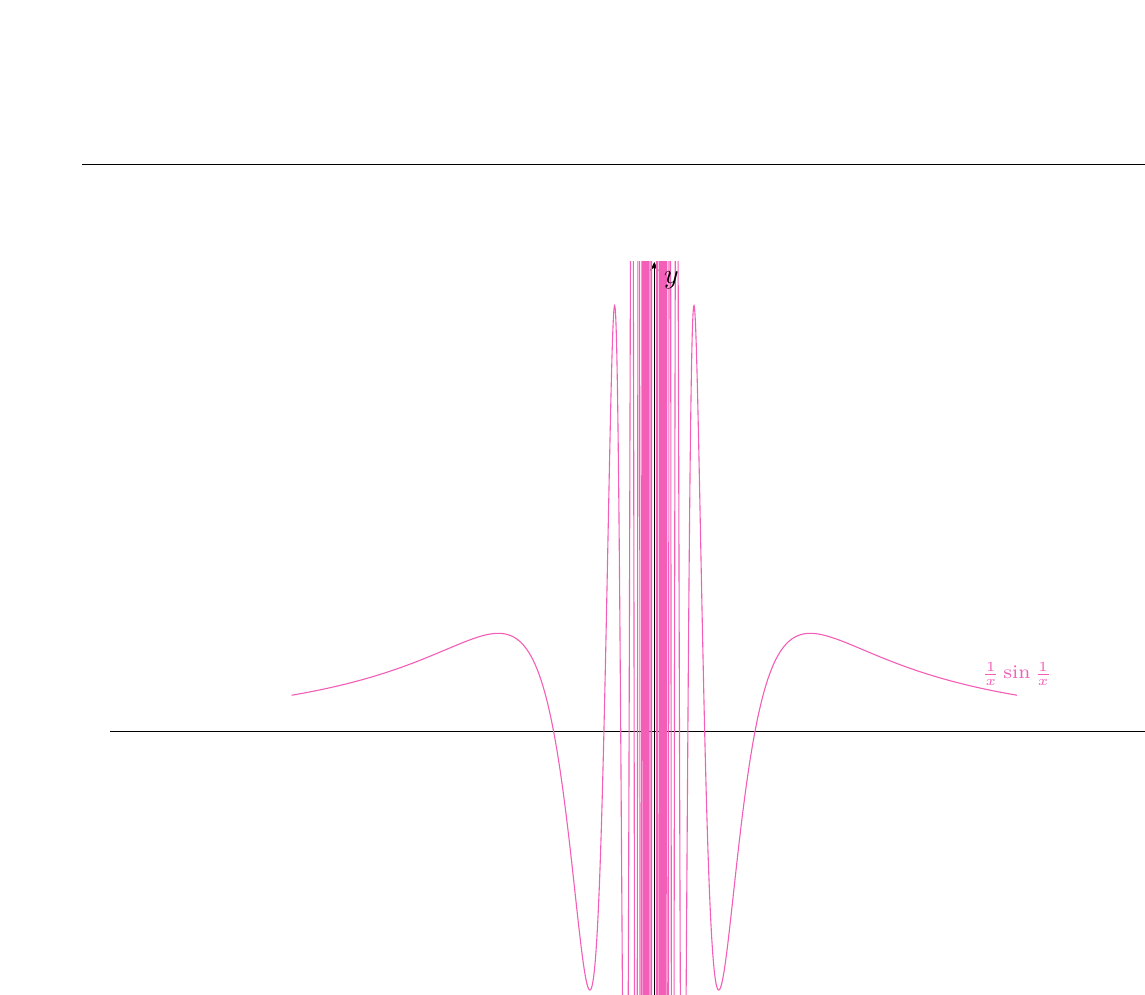
\begin{tikzpicture}
        \begin{axis}[
                ticks=none,
                axis lines=middle,
                ymin=-500,
                ymax=500,
                xmin=-0.03,
                xmax=0.03,
                xlabel=$x$,
                ylabel=$y$,
                scale only axis,
                width=\textwidth
            ]
            \addplot[CarnationPink,domain=-0.02:-0.0001,samples=1000] {sin(1/x)/x};
            \addplot[CarnationPink,domain=0.0001:0.02,samples=1000] {sin(1/x)/x} node[above]{\scriptsize$\frac{1}{x}\sin\frac{1}{x}$};
        \end{axis}
    \end{tikzpicture}
    \caption{有界振荡和无界振荡}
\end{marginfigure}
\begin{definition}
    (间断点)函数$f(x)$在$x_0$处不连续,则称$x_0$为函数$f(x)$的间断点\\
    \begin{math}
        \begin{cases}
            \text{第一类间断点}
            \begin{cases}
                \text{可去间断点}\qquad (\text{左右极限相等}) \\
                \text{跳跃间断点}\qquad (\text{左右极限不等})
            \end{cases}
            \qquad (\text{左右极限存在})
            \\
            \text{第二类间断点}
            \begin{cases}
                \text{无穷间断点}\qquad (\text{无穷大}\frac{1}{x}) \\
                \text{振荡间断点}\qquad (\text{振荡}\sin\frac{1}{x})
            \end{cases}
            \qquad (\text{左极限或右极限不存在})
        \end{cases}
    \end{math}
\end{definition}
间断点不是无穷大则说明了,此间断点左右极限存在,或振荡(可有界如$\sin \frac{1}{x}$在$x=0$处,或无界如$\frac{1}{x}\sin \frac{1}{x}$)


\subsection{一致连续}
.
\begin{definition}
    \label{def:一致连续}
    (一致连续)
    $\forall \varepsilon>0,\exists \delta>0, \text{ 当~}x,y\in I \text{ 且~} \lvert x-y\rvert< \delta \text{ 时,恒有}$
    \[ \left\lvert f(x)-f(y)\right\rvert<\varepsilon \]
\end{definition}
\begin{theorem}
    若函数$f(x)$的一阶导数$f'(x)$有界,则函数$f(x)$一致连续。(可通过中值定理得证)
\end{theorem}
\begin{proof}
    因为$\left\lvert f'(x) \right\rvert < M$,根据中值定理,对于定义域内任意的$a,b,\lvert a-b \rvert < \delta$,令$\delta=\frac{\varepsilon}{M}$可得
    \[
        \left\lvert f(a) - f(b) \right\rvert
        = \left\lvert f'(\xi)(a-b) \right\rvert
        < M\left\lvert a-b \right\rvert
        < M\delta = \varepsilon
    \]
\end{proof}

\subsection{闭区间上连续函数的性质}
此性质的考察通常出现与选择题、证明题中。
\begin{theorem}
    (有界性定理)闭区间上的连续函数一定是有界函数
\end{theorem}
\begin{theorem}
    (最值定理)闭区间上的连续函数一定有最大值和最小值
\end{theorem}
\begin{theorem}
    (介值定理)若$C$介于$f(a),f(b)$,则一定有$f(\xi)=C \qquad (\xi\in[a,b])$
\end{theorem}
\begin{theorem}
    (零点定理)若闭区间$[a,b]$上的连续函数$f(x)$,有$f(a)f(b)<0$则一定有$f(\xi)=0 \qquad (\xi\in(a,b))$
\end{theorem}
\begin{theorem}
    (一致连续定理)闭区间上的连续函数必一致连续\ref{def:一致连续}
\end{theorem}


% \part{导数}
\section{基本概念}
.
\begin{definition}
    若函数$f(x)$在某点$x_0$的领域内有定义,并且有
    \[ f'(x) = \lim_{x \to x_0} \frac{f(x)-f(x_0)}{x-x_0} \]
    则函数$f(x)$在$x_0$处可导。
\end{definition}

\begin{theorem}
    函数$f(x)$在$x_0$处可导且$f(x_0) = A \iff$函数$f(x)$在$x_0$点单侧可导
    且$f'_-(x_0)=f'_+(x_0)=A$
\end{theorem}


\section{求导法则}
导数的四则运算如下
\begin{theorem}
    设函数$u(x), v(x)$均在$(a,b)$内可导,则函数$u(x), v(x)$的和、差、积、商(分母不为零)均在$(a,b)$内可导,并且有
    \begin{align}
        \left[u(x) \pm v(x) \right]'      & = u'(x) \pm v'(x)                      \\
        \left[ u(x) \cdot v(x) \right]'   & = u'(x)v(x) + u(x)v'(x)                \\
        \left[ \frac{u(x)}{v(x)} \right]' & = \frac{u'(x)v(x) - u(x)v'(x)}{v^2(x)}
    \end{align}
\end{theorem}

\begin{theorem}
    (反函数求导法则)
    \label{th:反函数求导法则}
    设函数$\varphi (y)$可导,如果$\varphi'(y) \neq 0$,则反函数$y=f(x)$可导.
    \[ f'(x) = \dv{y}{x} = \left. 1 \middle / \dv{x}{y}\right. = \frac{1}{\varphi'(y)} = \frac{1}{\varphi'(f(x))} \]
\end{theorem}
复合函数求导如下
\begin{theorem}
    (链式法则)
    \label{th:链式法则}
    设函数$y=f(u)$与函数$u=\varphi(x)$均可导,则符合函数$y=f(\varphi(x))$在其定义域内可导,并且有$(f\circ\varphi)'(x)=f'(\varphi(x))\cdot\varphi'(x)$即
    \[ \dv{y}{x} = \dv{y}{u} \cdot \dv{u}{x} \]
\end{theorem}

\subsection{高阶导数}
在求高阶导数的通式和值时,主要使用Leibiz公式,对于不是很好求的函数时,可对部分项进行泰勒展开。
\begin{theorem}
    (Leibniz公式)
    \label{th:Leibniz公式}
    设$u=u(x),v=v(x)$在$x$点处有$n$阶导数,则
    \[ (uv)^{(n)} = \sum^n_{k=0}C^k_n u^{(n-k)}v^{(k)} \]
\end{theorem}

\begin{example}
    已知$y=x^2\sin 2x$,求$y^{(50)}$
\end{example}
\begin{solution}
    根据Leibniz公式\ref{th:Leibniz公式},可得
    \begin{align}
        y^{(50)} & = \sum_{n=0}^{50} C_{50}^n (x^2)^{(n)}\cdot(\sin 2x)^{(50-n)}                                                       \\
                 & = C_{50}^0(x^2)\cdot(\sin 2x)^{(50)} + C_{50}^1(x^2)'\cdot(\sin 2x)^{(49)} + C_{50}^2(x^2)''\cdot(\sin 2x)^{(48)}+0 \\
                 & = 2^{50}\cdot \left[ x^2 \sin(2x+25\pi) + 50x\sin(2x+\frac{49\pi}{2})+\frac{25 \cdot 49}{2}\sin(2x+24\pi) \right]   \\
                 & = 2^{50}\cdot\left[ -x^2\sin 2x + 50x\cos 2x + \frac{1225}{2}\sin 2x \right]
    \end{align}
\end{solution}

\begin{example}
    已知
    \begin{math}
        y =
        \begin{cases}
            \frac{\sin x}{x}, & x \neq 0 \\
            1,                & x = 0
        \end{cases}
    \end{math}
    求$y^{(n)}(0)$
\end{example}
\begin{solution}
    当$x\neq 0$时,由泰勒展开可得
    \begin{align}
        y & = \frac{1}{x}(x - \frac{x^3}{3!} + \frac{x^5}{5!} - \cdots) \\
          & = 1-\frac{x^2}{3!}+\frac{x^4}{5!}-\cdots                    \\
          & =\sum_{k=0}^\infty \frac{(-1)^{k}x^{2k}}{(2k+1)!}
    \end{align}
    同时有
    \[ \lim_{x \to 0} \sum_{k=0}^\infty \frac{(-1)^{k}x^{2k}}{(2k+1)!} = 1 \]
    所以对于$(-\infty,+\infty)$,泰勒展开恒成立。
    又由于
    \[ y = \sum_{n=0}^{\infty}\frac{y^{(n)}}{n!}x^{n} \]
    比较系数可得
    \[
        y^{(n)}(0) =
        \begin{cases}
            0,                      & n = 2k+1, \\
            \dfrac{(-1)^{k}}{2k+1}, & n=2k
        \end{cases}
    \]
\end{solution}

\section{微分中值定理}
微分中值定理属于重要且必考的定理,常出现于证明题中。
\begin{theorem}
    (罗尔定理)
    \label{th:罗尔定理}
    设函数$f(x)$在区间$[a,b]$上连续,$(a,b)$内可导,
    且$f(a)=f(b)$,则有
    \[ f'(\xi) = 0 \qquad \xi \in (a,b)\]
\end{theorem}

\begin{theorem}
    (拉格朗日中值定理)
    \label{th:拉格朗日中值定理}
    设函数$f(x)$在区间$[a,b]$上连续,$(a,b)$内可导,则有
    \[ \frac{f(b)-f(a)}{b-a} = f'(\xi) \qquad \xi \in (a,b)\]
\end{theorem}

\begin{theorem}
    (柯西中值定理)
    \label{th:柯西中值定理}
    设函数$f(x),g(x)$在区间$[a,b]$上连续,$(a,b)$内可导,且$g'(x)\neq0$恒成立,则有
    \[ \frac{f(b)-f(a)}{g(b)-g(a)} = \frac{f'(\xi)}{g'(\xi)} \qquad \xi \in (a,b)\]
\end{theorem}

\begin{example}
    设$f(x)$在$[a,b]$上连续,$f''(x)$在$(a,b)$存在。连接点$(a,f(a)),(b,f(b))$交曲线$y=f(x)$于点$(c,f(c))$,且$a<c<b$,
    证明存在$\xi\in(a,b)$使得$f''(\xi)=0$.
\end{example}
\begin{proof}
    根据拉格朗日中值定理得
    \begin{align*}
        \frac{f(c)-f(a)}{c-a} & = f'(\xi_1) & \xi_1 \in (a,c) \\
        \frac{f(b)-f(c)}{b-c} & = f'(\xi_2) & \xi_2 \in (c,b)
    \end{align*}
    而由于点$(a,f(a)),(c,f(c)),(b,f(b))$共线,所以有
    \[ f'(\xi_1) = f'(\xi_2) \qquad \xi_1,\xi_2 \in (a,b) \]
    根据罗尔定理可知
    \[ f''(\xi) = 0  \qquad \xi \in (\xi_1,\xi_2) \subseteq (a,b) \]
\end{proof}


\begin{example}
    设函数$f(x)$在区间$[a,b]$上连续,$(a,b)$内可导,且$f'(x)\neq 0$,试证存在$\xi,\eta \in (a,b)$使得
    \[ \frac{f'(\xi)}{f'(\eta)} = \frac{\mathrm{e}^b-\mathrm{e}^a}{b-a}\mathrm{e}^{-\eta} \]
\end{example}

\begin{proof}
    根据柯西中值定理可得
    \[ \frac{f(b)-f(a)}{\mathrm{e}^b-\mathrm{e}^a} = \frac{f'(\eta)}{\mathrm{e}^\eta} \qquad \eta \in (a,b) \]
    根据拉格朗日中值定理得
    \[ \frac{f(b)-f(a)}{b-a} = f'(\xi) \qquad \xi \in (a,b) \]
    因此有
    \[ f(b)-f(a) = \left( \mathrm{e}^b - \mathrm{e}^a \right)f'(\eta)\mathrm{e}^{-\eta}=(b-a)f'(\xi)  \qquad \xi,\eta \in (a,b) \]
    变形得
    \[ \frac{f'(\xi)}{f'(\eta)} = \frac{\mathrm{e}^b-\mathrm{e}^a}{b-a}\mathrm{e}^{-\eta} \qquad \xi,\eta \in (a,b) \]
\end{proof}

\begin{example}
    设函数$f(x)$在$[a,b]$上连续,在$(a,b)$内可导,且$f(a)=f(b)=0$,求证:
    \begin{enumerate}[(1)]
        \item 存在$\xi\in(a,b)$,使$f(\xi)+\xi f'(\xi)=0$;
        \item 存在$\eta\in(a,b)$,使$\eta f(\eta) + f'(\eta)=0$;
    \end{enumerate}
\end{example}
\begin{proof}
    \begin{enumerate}[(1)]
        \item 设$g(x)=xf(x)$,则由罗尔定理得,存在$\xi\in(a,b)$使得
              \[ g'(\xi)=f(\xi)+\xi f'(\xi)=0 \]
        \item 设$h(x)=\mathrm{e}^{\frac{x^2}{2}}f(x)$,则由罗尔定理得,存在$\eta\in(a,b)$使得
              \[ h'(\eta) = \mathrm{e}^{\frac{\eta^2}{2}}(\eta f(\eta)+f'(\eta)) = 0 \]
              即
              \[ \eta f(\eta) + f'(\eta)=0 \]
    \end{enumerate}
\end{proof}
常见的构造函数如下:
\begin{alignat*}{2}
     & g(x)=xf(x),                           & \qquad & g'(x)=f(x)+xf'(x)                                  \\
     & g(x)=\dfrac{f(x)}{x},                 & \qquad & g'(x) = \dfrac{xf'(x)-f(x)}{x^2}, (x\neq 0)        \\
     & g(x)=\mathrm{e}^{m(x)}f(x),           & \qquad & g'(x) = \mathrm{e}^{m(x)}(m'(x)f(x)+f'(x))         \\
     & g(x)=\dfrac{f(x)}{\mathrm{e}^{m(x)}}, & \qquad & g'(x) = \dfrac{f'(x)-m'(x)f(x)}{\mathrm{e}^{m(x)}} \\
\end{alignat*}
前两个的$f(x)$系数为$\pm1$,后两个则是$f'(x)$的系数为$1$。

当无法猜出$g(x)$时,可以考虑$\frac{m'(x)}{n'(x)}$,根据柯西中值定理来推出$m(x)$和$n(x)$。

\begin{example}
    设函数$f(x)$在$[a,b]$上连续,在$(a,b)$内可导,且$f(a)\neq f(b)$,求证:$\exists \xi,\eta \in (a,b)$使得
    \[ \frac{f'(\xi)}{2\xi} = \frac{f'(\eta)}{b+a} \]
\end{example}
\begin{proof}
    因为
    \[ \frac{f'(\xi)}{2\xi}, \qquad \frac{f'(\eta)}{b+a} = \frac{f'(\eta)(b-a)}{b^2-a^2} \]
    所以可以猜测需要柯西中值定理以及涉及两个函数$f(x)$和$x^2$,所以有
    \[ \frac{f(b)-f(a)}{b^2-a^2} = \frac{f'(\xi)}{2\xi}, \qquad \xi\in(a,b) \]
    注意到
    \[ \frac{f(b)-f(a)}{b^2-a^2} = \frac{f(b)-f(a)}{(b-a)(b+a)} = \frac{f'(\eta)}{b+a}, \qquad \eta\in(a,b)\]
    所以有
    \[ \frac{f'(\xi)}{2\xi} = \frac{f'(\eta)}{b+a}, \qquad \xi,\eta\in(a,b) \]
\end{proof}


\section{泰勒展开}
泰勒公式不仅可以用于求解极限,还能证明与导数相关的题目。
\begin{example}
    设$f(x)$在$x_0$处$n$阶可导,且$f^{(m)}(x)=0,(m=1,2,\cdots,n-1),f^{(n)}(x)\neq 0(n\geq 2)$,证明:
    \begin{enumerate}[(1)]
        \item 当$n$为偶数且$f^{(n)}(x_0)<0$时,$f(x)$在$x_0$取得极小值;
        \item 当$n$为偶数且$f^{(n)}(x_0)>0$时,$f(x)$在$x_0$取得极大值;
    \end{enumerate}
\end{example}
\begin{proof}
    根据泰勒公式可知:
    \begin{align*}
        f(x) & = f(x_0) + \sum_{k=1}^{n-1} \frac{f^{(k)}(x_0)}{k!}(x-x_0)^k + \frac{f^{(n)}(\xi)}{n!}(x-x_0)^n \\
             & = f(x_0) +  \frac{f^{(n)}(\xi)}{n!}(x-x_0)^n
    \end{align*}
    其中$\xi$位于$x_0$的去心领域内。

    当$n$为偶数且$f^{(n)}(x_0)<0$时,$x_0$的去心领域内有,$f(x) \leq f(x_0)$,则$f(x)$在$x_0$取得极小值;

    当$n$为偶数且$f^{(n)}(x_0)>0$时,$x_0$的去心领域内有,$f(x) \geq f(x_0)$,则$f(x)$在$x_0$取得极大值。
\end{proof}

\begin{example}
    若函数$\varphi(x)$及$\psi(x)$是$n$阶可微的,且$\varphi^{(k)}(x_0)=\psi^{(k)}(x_0),k=0,1,2,\cdots,n-1$,又$x>x_0$时,
    $\varphi^{(n)}(x)>\psi^{(n)}(x)$。试证:当$x>x_0$时,$\varphi(x)>\psi(x)$
\end{example}
\begin{proof}
    根据泰勒公式可知
    \[ \varphi(x) = \sum_{k=0}^{n-1}\frac{\varphi^{(k)}(x_0)}{k!}(x-x_0)^k + \frac{\varphi^{(n)}(\xi_1)}{n!}(x-x_0)^n \]
    \[ \psi(x) = \sum_{k=0}^{n-1}\frac{\psi^{(k)}(x_0)}{k!}(x-x_0)^k + \frac{\psi^{(n)}(\xi_2)}{n!}(x-x_0)^n \]
    当$x>x_0$时,$\xi_1,\xi_2\in(x_0,x)$,此时由上述两个等式可得
    \[ \varphi(x) - \psi(x) = \frac{(x-x_0)^n}{n!}[\varphi^{(n)}(\xi_1) - \psi^{(n)}(\xi_2)] > 0\]
    因此当$x>x_0$时,$\varphi(x)>\psi(x)$
\end{proof}

\section{导数的应用}
\subsection{极值求解}
极值的定义如下
\begin{definition}
    极大值与极小值(统称极值)是指在一个域上函数取得最大值(或最小值)的点的函数值。而使函数取得极值的点(的横坐标)被称作极值点。这个域既可以是一个邻域,又可以是整个函数域(这时极值称为最值)
    若某点连续且左右两侧的单调性相异,则该点为极值点。
\end{definition}
\begin{theorem}
    当$f'(x_0)=0$时
    \begin{enumerate}
        \item 当$f(x)$在$x_0$连续,且$f'_-(x_0)<0,f'_+(x_0)>0$时, $x_0$为极小值点
        \item 当$f(x)$在$x_0$连续,且$f'_-(x_0^)>0,f'_+(x_0)<0$时, $x_0$为极大值点
        \item $f''(x_0)>0,\ x_0$为极小值点
        \item $f''(x_0)<0,\ x_0$为极大值点
    \end{enumerate}
\end{theorem}

\subsection{零点的求解}
对于函数$f(x)$,零点的存在性由介值定理得出。零点位置、个数要根据函数的变化(单调性,水平渐近线)来进行求解。
\begin{theorem}
    介值定理
    \label{th:介值定理}
    若函数$f(x)$在$[a,b]$上连续,且$f(a)<f(b)$,若$\forall u$满足$f(a)<u<f(b)$,则至少存在一点$x=c$且$a<c<b$,使得$f(c)=u$。$f(a)>f(b)$同理。
\end{theorem}

\begin{example}
    讨论方程$ax\mathrm{e}^x+b=0,(a>0)$的实根情况。
\end{example}
\begin{marginfigure}
    \begin{tikzpicture}
        \begin{axis}[
                ticks=none,
                axis x line=none,
                axis y line=middle,
                ymax=5,
                ymin=1,
                xmin=-10,
                xmax=10,
                domain=-10:10,
                xlabel=$x$,
                ylabel=$y$,
                scale only axis,
                width=\textwidth
            ]
            \addplot[CarnationPink,smooth,domain=-10:1] {exp(1)*x*exp(x)+3} node [right,pos=0.65,scale=0.7] {$ax\mathrm{e}^x+b$};
            \addplot[Gray,dashed,name path = L1] {3.05};
            \addplot[Gray,name path = L2] {2};
            \path[name path=YMax] (-10,5) -- (10,5);
            \path[name path=YMin] (-10,1) -- (10,1);
            \addplot [thick,color=red,fill=red,fill opacity=0.05]fill between[of=YMax and L1];
            \addplot [thick,color=blue,fill=blue,fill opacity=0.05]fill between[of=L1 and L2];
            \addplot [thick,color=green,fill=green,fill opacity=0.05]fill between[of=L2 and YMin];
            \node [Gray, scale=0.7] at (8,1.5) {无实根};
            \node [Gray, scale=0.7] at (8,2.5) {两个实根};
            \node [Gray, scale=0.7] at (8,4) {一个实根};
            \node [Gray, scale=0.7] at (8,2) {一个实根};
        \end{axis}
    \end{tikzpicture}
\end{marginfigure}
\begin{solution}
    令$f(x) = ax\mathrm{e}^x+b$,则有
    \[
        \lim_{x\to-\infty}f(x)
        = a\lim_{x\to-\infty} x\mathrm{e}^x + b
        = a\lim_{x\to-\infty} \frac{x}{\mathrm{e}^{-x}} + b
        = a\lim_{x\to-\infty} \frac{1}{-\mathrm{e}^{-x}} + b
        = b
    \]
    \[
        \lim_{x\to+\infty}f(x) = +\infty
    \]
    对函数$f'(x)=a\mathrm{e}^x(1+x)=0$进行求解,得$x=-1$,则函数得单调性如下
    \begin{center}
        \begin{tabular}{|c|c|c|c|}
            \hline
            $x$     & $(-\infty,-1)$ & $-1$                      & $(-1,+\infty)$ \\ \hline
            $f'(x)$ & $-$            & $0$                       & $+$            \\ \hline
            $f(x)$  & $\searrow$     & $-\frac{a}{\mathrm{e}}+b$ & $\nearrow$     \\ \hline
        \end{tabular}
    \end{center}
    所以
    \begin{enumerate}
        \item 当$0 < -\frac{a}{\mathrm{e}}+b$时,即$b\in(-\frac{a}{\mathrm{e}},+\infty)$,方程无实根。
        \item 当$0 = -\frac{a}{\mathrm{e}}+b$或$0 \geq b$时,即$b\in(-\infty,0]\cup \left\{ -\frac{a}{\mathrm{e}} \right\}$,方程有一实根。
        \item 当$-\frac{a}{\mathrm{e}}+b < 0 < b$时,即$b\in(0,-\frac{a}{\mathrm{e}})$,方程有两个不同的实根。
    \end{enumerate}
\end{solution}

对于求$f(x)$的极值步骤如下
\begin{enumerate}
    \item 确定定义域
    \item 计算导函数$f'(x)$
    \item 求解方程$f'(x)=0$(根可能为临界点)
    \item 确定可能的极值点(临界点、\textcolor{red}{不可导点})
    \item 按照极值的充分性判断极值点
    \item 计算极值点的函数值,得出极值
\end{enumerate}

\begin{example}
    求函数$y=(x^2-1)^{2/3}$的极值。
\end{example}
\begin{solution}
    由
    \[ y'=\frac{4}{3}\frac{x}{\sqrt[3]{x^2-1}}=0 \]
    解得临界点$x=0$和不可导点$x=\pm 1$
    因此可得如下情况:
    \begin{center}
        \begin{tabular}{|c|c|c|c|c|c|c|c|}
            \hline
            $x$  & $(-\infty,1)$ & $-1$     & $(-1,0)$   & $0$      & $(0,1)$    & $1$    & $(1,+\infty)$ \\ \hline
            $y'$ & $-$           & 不存在   & $+$        & $0$      & $-$        & 不存在 & $+$           \\ \hline
            $y$  & $\searrow$    & $\smile$ & $\nearrow$ & $\frown$ & $\searrow$ & 极小值 & $\nearrow$    \\ \hline
        \end{tabular}
    \end{center}
    故函数$y=(x^2-1)^{2/3}$有极大值$\eval{y}_{x=0}=1$,有极小值$\eval{y}_{x=\pm 1}=0$
\end{solution}

\subsection{函数的凹凸性}
当函数弦在上,曲在下,函数称为凹函数(反之则为凸函数)。以数学的语言,即如下不等式成立时,函数为凹函数
\begin{definition}
    设函数$f(x)$在区间$(a,b)$内有定义,如果$x_1,x_2\in(a,b), t \in [0,1]$时,恒有
    \[ f((1-t)x_1+tx_2)\leq (1-t)f(x_1)+tf(x_2) \]
    则函数$f(x)$在区间$(a,b)$为凹函数。
\end{definition}
换句话说,组合的像小于等于像的组合时,函数为凹函数

\begin{theorem}
    设函数$f(x)$在区间$[a,b]$上连续,在$(a,b)$内二阶可导,则
    \begin{enumerate}
        \item 当$f''(x)>0$于$(a,b)$时,$f(x)$是$[a,b]$上的严格凹函数
        \item 当$f''(x)<0$于$(a,b)$时,$f(x)$是$[a,b]$上的严格凸函数
        \item 若该函数在某点的二阶导数为零或不存在,且二阶导数在该点两侧符号相反,该点即为函数的拐点。
    \end{enumerate}
\end{theorem}

\subsection{函数的曲率}
曲率的几何概念可由右图给出
\begin{marginfigure}
    \centering
    \begin{tikzpicture}
        \begin{axis}[
                ticks=none,
                disabledatascaling,
                axis lines=middle,
                xmin=0,
                xmax=8,
                ymin=0,
                ymax=8,
                domain=0:8,
                xlabel=$x$,
                ylabel=$y$,
                scale only axis,
                unit vector ratio=1 1,
                width=\textwidth
            ]
            \pgfmathsetmacro{\cx}{4}
            \pgfmathsetmacro{\cy}{4}
            \pgfmathsetmacro{\r}{3}
            \pgfmathsetmacro{\a}{30}
            \pgfmathsetmacro{\da}{30}

            \coordinate (C) at ({\cx},{\cy});
            \coordinate (A) at ({\r*sin(\a)+\cx},{\cy-\r*cos(\a)});
            \coordinate (B) at ({\r*sin(\a+\da)+\cx},{\cy-\r*cos(\a+\da)});
            \node at (C) [above right] {$\textcolor{red}{\Delta\alpha}$};
            \draw [name path=circle] (C) circle [radius={\r}];
            \draw (A) -- (C) node [left,pos=0.3] {$R$} -- (B) pic [draw=Gray] {angle=A--C--B};
            \addplot [name path =L1, Gray] {tan(\a) * (x-\r*sin(\a)-\cx) + \cy - \r*cos(\a)};
            \addplot [name path =L2, Gray] {tan(\a+\da) * (x-\r*sin(\a+\da)-\cx) + \cy - \r*cos(\a+\da)};
            \path [name intersections={of=L1 and L2}];
            \coordinate (D) at (intersection-1);
            \coordinate (E) at (8, {tan(\a) * (8-\r*sin(\a)-\cx) + \cy - \r*cos(\a)});
            \pic [draw=Gray,"$\textcolor{red}{\Delta\alpha}$", angle radius=15, angle eccentricity=1.5] {angle=E--D--B};
            \coordinate (X) at (8,0);
            \path [name path=XAxis] (0,0)--(X);
            \path [name intersections={of=L1 and XAxis}];
            \coordinate (F) at (intersection-1);
            \path [name intersections={of=L2 and XAxis}];
            \coordinate (G) at (intersection-1);
            \pic [draw=Gray,"$\alpha$", angle radius=15, angle eccentricity=1.5] {angle=X--F--D};
            \pic [draw=Gray,"$\alpha+\textcolor{red}{\Delta\alpha}$", angle radius=15, angle eccentricity=2] {angle=X--G--D};
            \draw [very thick, blue] (A) arc[radius={\r}, start angle={\a-90}, end angle={\a+\da-90}] node [left, pos=0.8] {$\Delta s$};
        \end{axis}
    \end{tikzpicture}
    \caption{某段曲线的曲率变化}
\end{marginfigure}

\begin{definition}
    (曲率$K$和曲率半径$R$)
    \begin{align*}
        R & = \lim_{\Delta\alpha\to 0} \abs{\frac{\Delta s}{\Delta \alpha}} = \abs{\dv{s}{\alpha}} &                 \\
        \\
        K & = \frac{1}{R} = \abs{\dv{\alpha}{s}}                                                   & \text{定义式}   \\
          & =\frac{\abs{y''}}{[1+y'^2]^{3/2}}                                                      & \text{函数形式} \\
          & =\frac{\abs{x'y''-x''y'}}{[x'^2+y'^2]^{3/2}}                                           & \text{参数形式}
    \end{align*}
\end{definition}

\begin{proof}
    如果曲线$L$的方程$y=f(x)$具有二阶导数,则
    \[ \alpha = \arctan y',\dd{\alpha}=\frac{y''}{1+y'^2}\dd{x} \]
    根据弧长公式$\dd{s}=\sqrt{\dd{x^2} + \dd{y^2}} = \sqrt{1+y'^2}\dd{x}$,可得
    \[ K = \frac{\abs{y''}}{[1+y'^2]^{3/2}} \]
\end{proof}

\begin{example}
    已知$f(x)$二阶可导,且$f(x)>0,f(x)f''(x)-[f'(x)]^2 \geq 0 (x\in \mathbf{R})$,
    证明
    \[f(x_1)f(x_2)\geq f^2\left(\frac{x_1+x_2}{2}\right)\ (x_1,x_2\in \mathbf{R})\];
\end{example}

\begin{proof}
    令$g(x)=\ln f(x)$,则
    \[g''(x) = \frac{f(x)f''(x)-[f'(x)]^2}{f^2(x)} \geq 0 \]
    所以$g(x)$为凹函数,所以有
    \[ \frac{1}{2}[g(x_1)+g(x_2)] \geq g\left(\frac{x_1+x_2}{2}\right) \]
    即
    \[f(x_1)f(x_2)\geq f^2\left(\frac{x_1+x_2}{2}\right)\]
\end{proof}


\subsection{渐近线}
渐近线分为\textcolor{red}{水平渐近线}、\textcolor{red}{垂直渐近线}、\textcolor{red}{斜渐近线}。如下图
\begin{figure}[htbp]
    \centering
    \begin{subfigure}[b]{0.3\linewidth}
        \begin{tikzpicture}
            \begin{axis}[
                    ticks=none,
                    axis lines=middle,
                    ymin=-pi,
                    ymax=pi,
                    xlabel=$x$,
                    ylabel=$y$,
                    scale only axis,
                    width=\textwidth
                ]
                \addplot[CarnationPink, smooth] {rad(atan(x))};
                \addplot[Gray, dashed] {pi/2} node [midway, left, text=black] {$\frac{\pi}{2}$};
                \addplot[Gray, dashed] {-pi/2} node [midway, left, text=black] {$-\frac{\pi}{2}$};
            \end{axis}
        \end{tikzpicture}
        \subcaption{$\textcolor{CarnationPink}{\arctan x}$的水平渐近线}
    \end{subfigure}
    \begin{subfigure}[b]{0.3\linewidth}
        \begin{tikzpicture}
            \begin{axis}[
                    ticks=none,
                    axis lines=middle,
                    ymin=-4.5,ymax=4.5,
                    xmin=-pi,xmax=pi,
                    xlabel=$x$,
                    ylabel=$y$,
                    scale only axis,
                    width=\textwidth
                ]
                \addplot[CarnationPink, smooth, domain=-pi/2:pi/2] {tan(deg(x))};
                \addplot[CarnationPink, smooth, domain=-pi:-pi/2] {tan(deg(x))};
                \addplot[CarnationPink, smooth, domain=pi/2:pi] {tan(deg(x))};
                \addplot[Gray, dashed, variable=\y, domain=-4.5:4.5] (pi/2, {\y}) node [midway, below left,text=black] {$\frac{\pi}{2}$};
                \addplot[Gray, dashed, variable=\y, domain=-4.5:4.5] (-pi/2, {\y}) node [midway, below left,text=black] {$-\frac{\pi}{2}$};
            \end{axis}
        \end{tikzpicture}
        \subcaption{$\textcolor{CarnationPink}{\tan x}$的垂直渐近线}
    \end{subfigure}
    \begin{subfigure}[b]{0.3\linewidth}
        \begin{tikzpicture}
            \begin{axis}[
                    ticks=none,
                    axis lines=middle,
                    ymin=-pi,
                    ymax=2*pi,
                    xlabel=$x$,
                    ylabel=$y$,
                    scale only axis,
                    unit vector ratio=1 1,
                    width=\textwidth
                ]
                \addplot[CarnationPink, smooth] {x+rad(90-atan(x))};
                \addplot[Gray, dashed] {x} node [below right, pos=0.7, text=black] {$y=x$};
                \addplot[Gray, dashed] {x+pi} node [above left, pos=0.5, text=black] {$y=x+\pi$};
            \end{axis}
        \end{tikzpicture}
        \subcaption{$\textcolor{CarnationPink}{x + \arccot x}$的斜渐近线}
    \end{subfigure}
    \caption{三种渐近线}
\end{figure}

寻找渐进线的步骤为:
\begin{enumerate}
    \item 确定函数的间断点,判断间断点处是否存在垂直渐近线。
    \item 当函数在$x\to\infty$、$x\to-\infty$、$x\to+\infty$存在极限值时,函数存在水平渐近线(此时对应的$x$则没有斜渐近线)。
    \item 若$x\to\infty$、$x\to-\infty$、$x\to+\infty$时下式成立,则斜渐近线存在。
          \sidenote{其中函数曲线到斜渐近线的距离为\[d(x) = \dfrac{\abs{f(x)-kx-b}}{\sqrt{1+k^2}} \]}
          \[ \frac{f(x)}{x}\to k, \qquad f(x)-kx\to b \]
\end{enumerate}

% \part{一元积分}

\section{定积分}
\subsection{性质}
利用梯形逼近,定积分的定义如下
\begin{definition}
    设函数$f(x)$在闭区间$[a,b]$上有定义,如果存在$[a,b]$上的阶梯函数数列$\alpha_n(x),\beta_n(x)$使得
    \begin{enumerate}[(1)]
        \item 当$x\in[a,b]$且$n\geq 1$时,恒有$\alpha_n(x)\leq f(x)\leq \beta_n(x)$
        \item $\lim_{n\to\infty} \int_a^b \alpha_n(x)\dd{x} = \lim_{n\to\infty}\int_a^b \beta_n(x)\dd{x} = I$
    \end{enumerate}
    那么函数$f(x)$在$[a,b]$上的定积分为$\int_a^b f(x)\dd{x} = I$
\end{definition}

对于计算定积分,通常通过寻找原函数,再利用Newton-Leibniz公式计算。
\begin{theorem}
    (Newton-Leibniz公式)
    \label{th:Newton-Leibniz公式}
    如果函数$F(x)$是连续函数$f(x)$再区间$[a,b]$上的一个原函数,则
    \[ \int_a^bf(x)\dd{x} = F(b)-F(a) \]
\end{theorem}

可积函数的性质如下
\begin{theorem}
    函数$f(x)$在$[a,b]$上可积$\iff$对$\forall \epsilon > 0$,都$\exists [a,b]$上的阶梯函数
    $\alpha_n(x)$和$\beta_n(x)$使得
    \begin{enumerate}[(1)]
        \item 当$x\in[a,b]$时,恒有$\alpha_n(x)\leq f(x)\leq \beta_n(x)$
        \item $\int_a^b [\beta_n(x)-\alpha_n(x)] \dd{x} < \epsilon$
    \end{enumerate}
    推论:可积函数一定是有界函数
\end{theorem}

\begin{theorem}
    \marginnote{
        有界函数不一定可积,例如
        \[
            f(x) = \begin{cases}
                1, & x\text{ 为有理数} \\
                0, & x\text{ 为无理数}
            \end{cases}
        \]
        $f(x)$有界,但有无穷个间断点,故$f(x)$在任意的闭区间上不可积。
    }
    \begin{enumerate}
        \item 闭区间上的连续函数一定是可积函数。
        \item 闭区间上有界且最多只有\textcolor{red}{有限个}或\textcolor{red}{可数个}间断点的函数一定是可积函数。
        \item 闭区间上的单调有界函数一定是可积函数。
    \end{enumerate}
\end{theorem}

\begin{theorem}
    (积分线性性)
    设$f(x),g(x)$是$[a,b]$上的可积函数,$\lambda,\mu$是任意常数,
    则$f(x),g(x)$的线性组合$\lambda f(x)+\mu g(x)$是$[a,b]$上的可积函数,并且有
    \[
        \int_a^b \lambda f(x)+\mu g(x)\dd{x}
        =
        \lambda\int_a^b f(x)\dd{x} + \mu\int_a^b g(x)\dd{x}
    \]
\end{theorem}

\begin{theorem}
    (区间可加性)
    设函数$f(x)$是$[a,b]$上的可积函数,若$c\in(a,b)$,则
    \[ \int_a^b f(x)\dd{x} = \int_a^c f(x)\dd{x} + \int_c^b f(x)\dd{x} \]
\end{theorem}

\begin{theorem}
    (积分单调性)
    设$f(x),g(x)$是$[a,b]$上的可积函数,若$f(x)\leq g(x), \forall x \in (a,b)$则有
    \[ \int_a^b f(x)\dd{x} \leq \int_a^b g(x)\dd{x} \]

    推论:
    \begin{enumerate}[(1)]
        \item \[
                  \int_a^b f(x)\dd{x}
                  \begin{cases}
                      \geq 0 & f(x)\geq 0 \\
                      > 0    & f(x) > 0
                  \end{cases}
              \]
        \item 若$f(x),g(x)$不恒等,且$f(x)\leq g(x),\forall x \in (a,b)$,则有
              \[ \int_a^b f(x)\dd{x} < \int_a^b g(x)\dd{x} \]
        \item 若$m \leq f(x) \leq M$则有
              \[ m(b-a) \leq \int_a^b f(x)\dd{x} \leq M(b-a) \]
        \item 若$f(x)$非负,则对于子区间$[\alpha,\beta]$有
              \[ \int_\alpha^\beta f(x)\dd{x} < \int_a^bf(x)\dd{x} \]
    \end{enumerate}
\end{theorem}

\begin{theorem}
    (绝对可积性)
    \label{th:绝对可积性}
    设$f(x)$是$[a,b]$上的可积函数,则$\abs{f(x)}$在$[a,b]$上的可积函数,并且有
    \[ \abs{\int_a^b f(x)\dd{x}} \leq \int_a^b \abs{f(x)} \dd{x} \]
\end{theorem}

\begin{theorem}
    设$f(x)$在$[a,b]$上的连续函数,则存在$\xi\in(a,b)$,使得
    \[ \int_a^b f(x)\dd{x} = f(\xi)(b-a) \]
\end{theorem}

\begin{theorem}
    (积分中值定理)
    \label{th:积分中值定理}
    设$f(x)$在$[a,b]$上的连续函数,$g(x)$是$[a,b]$上的\textcolor{red}{不变号}可积函数,
    则$\exists \xi\in[a,b]$,使得
    \[ \int_a^b f(x)g(x)\dd{x} = f(\xi)\int_a^b g(x)\dd{x} \]
\end{theorem}

\subsubsection{奇偶函数、周期函数、含对称性函数、含有三角函数的定积分性质}
\paragraph{奇偶函数}
当定积分上下限对称,即积分区间为$[-a,a],a>0$时,奇偶函数$f(x)$的积分如下
\[
    \int_{-a}^a f(x)\dd{x} =
    \begin{cases}
        0,                   & f(x)\text{ 为奇函数} \\
        2\int_0^af(x)\dd{x}, & f(x)\text{ 为偶函数}
    \end{cases}
\]

\paragraph{周期函数}
当$f(x)$是以整数$T$为周期的连续函数,则对于任意的实数$a$,都有
\[\int_a^{a+T}f(x)\dd{x} = \int_0^T f(x)\dd{x} \]

\paragraph{含对称性函数}
若函数$f(x)$在$[a,b]$上可积,且$f(x)$关于$x=\dfrac{a+b}{2}$对称,那么可以令$t=x-\dfrac{a+b}{2}$
再根据偶函数的性质进行积分

当$f(x)$在$[a,b]$上可积时,且$f(x)$有某种轮换性质时,
可以通过$f(x)+f(a+b-x)$来简化定积分$\displaystyle\int_a^bf(x)\dd{x}$的计算。
其本质是在区间$[a,b]$上从左加到右,和从右加到左是一样的。
\begin{example}
    设$n$是正整数,计算$\displaystyle\int_0^{\frac{\pi}{2}}\frac{\sin^n x}{\sin^n x + \cos^n x}\dd{x}$
\end{example}
\begin{solution}
    令$t=\frac{\pi}{2}-x$,则有
    \begin{align*}
        \int_0^{\frac{\pi}{2}}\frac{\sin^n x}{\sin^n x + \cos^n x}\dd{x}
         & = \int_{\frac{\pi}{2}}^0\frac{\sin^n \left(\frac{\pi}{2}-t\right)}{\sin^n \left(\frac{\pi}{2}-t\right) + \cos^n \left(\frac{\pi}{2}-t\right)}\dd(\frac{\pi}{2}-t) \\
         & = \int_0^{\frac{\pi}{2}}\frac{\cos^n t}{\cos^n t + \sin^n t}\dd{t}
    \end{align*}
    根据$A = \frac{1}{2}(A+A)$可得
    \[
        \int_0^{\frac{\pi}{2}}\frac{\sin^n x}{\sin^n x + \cos^n x}\dd{x}
        =
        \frac{1}{2}\int_0^{\frac{\pi}{2}}\frac{\sin^n x + \cos^nx}{\sin^n x + \cos^n x}\dd{x}
        =
        \frac{1}{2}\int_0^{\frac{\pi}{2}} 1\dd{x}
        =
        \frac{\pi}{4}
    \]
\end{solution}

\begin{example}
    求定积分$\displaystyle\int_0^{\pi/2} \frac{1}{1+(\tan x)^{\sqrt{2}}}\dd{x}$
\end{example}
\begin{solution}
    \[
        \int_0^{\pi/2} \frac{1}{1+(\tan x)^{\sqrt{2}}}\dd{x}
        =
        \int_0^{\pi/2} \frac{(\cos x)^{\sqrt{2}}}{(\cos x)^{\sqrt{2}}+(\sin x)^{\sqrt{2}}}\dd{x}
    \]
    令$x=\frac{\pi}{2}-x$,则有
    \[
        \int_0^{\pi/2} \frac{(\cos x)^{\sqrt{2}}}{(\cos x)^{\sqrt{2}}+(\sin x)^{\sqrt{2}}}\dd{x}
        =
        \int_0^{\pi/2} \frac{(\sin x)^{\sqrt{2}}}{(\sin x)^{\sqrt{2}}+(\cos x)^{\sqrt{2}}}\dd{x}
    \]
    两式相加,则有
    \[
        \int_0^{\pi/2} \frac{1}{1+(\tan x)^{\sqrt{2}}}\dd{x}
        =
        \frac{1}{2} \int_0^{\pi/2} \frac{(\sin x)^{\sqrt{2}} + (\cos x)^{\sqrt{2}}}{(\sin x)^{\sqrt{2}}+(\cos x)^{\sqrt{2}}}\dd{x}
        =
        \frac{\pi}{4}
    \]
\end{solution}

\paragraph{含有三角函数}
设函数$f(x)$在$[0,1]$上连续,则有
\begin{enumerate}[(1)]
    \item $\displaystyle \int_0^{\pi/2}f(\sin x)\dd{x} = \int_0^{\pi/2}f(\cos x)\dd{x}$;
    \item $\displaystyle \int_0^{\pi}f(\sin x)\dd{x} = 2\int_0^{\pi/2}f(\sin x)\dd{x}$;
    \item $\displaystyle \int_0^{\pi}xf(\sin x)\dd{x} = \frac{\pi}{2}\int_0^{\pi}f(\sin x)\dd{x}$;
\end{enumerate}

\subsection{等式和不等式的证明}
含有积分的等式和不等式的证明,常用到以下几个知识点
\begin{enumerate}
    \item 积分中值定理(\ref{th:积分中值定理}),微分中值定理(\ref{th:罗尔定理}、\ref{th:拉格朗日中值定理}、\ref{th:柯西中值定理}),介值定理(\ref{th:介值定理})
    \item 泰勒公式(\ref{th:泰勒公式})
    \item 柯西不等式(\ref{eq:柯西不等式})、闵可夫斯基不等式(\ref{eq:闵可夫斯基不等式})
    \item 有绝对值时,绝对可积性(\ref{th:绝对可积性})、三角不等式(\ref{eq:三角不等式})、分段积分
    \item 将积分当作一个函数,研究其单调性和极值(最值)
    \item 被积函数的一些性质(单调性、周期性等)
\end{enumerate}
\begin{example}
    设函数$f(x)$在$[0,1]$上二阶可导,且$f(0)=f'(0)=f'(1)=0, f(1)=1$,
    证明:$\exists\xi\in(0,1)$,使得$\abs{f''(\xi)}\geq 4$
\end{example}
\begin{proof}
    注意到
    \begin{align*}
        f(b) - f(a) & = \int_a^b f'(x)\dd{x}                                                                \\
                    & = \int_a^b f'(x)\dd(x-t)                                                              \\
                    & = (b-t)f'(b)-(a-t)f'(a) - \int_a^b (x-t)f''(x)\dd{x} \qquad (\forall t\in \mathbf{R})
    \end{align*}
    当$f'(b)=f'(a)=0$时有
    \[ f(b) - f(a) = -\int_a^b (x-t)f''(x)\dd{x} \]
    由题意知$b=1,a=0$,由绝对可积性和积分中值定理可得
    \[
        1
        =
        \abs{\int_0^1 (x-t)f''(x)\dd{x}}
        \leq
        \int_0^1 \abs{x-t}\abs{f''(x)}\dd{x}
        = \abs{f''(\xi)}\int_0^1\abs{x-t}\dd{x}
    \]
    令$t=\frac{1}{2}$则有
    \[ 1 \leq \abs{f''(\xi)} \int_0^1\abs{x-\frac{1}{2}}\dd{x} = 4\abs{f''(\xi)} \qquad \xi\in(0,1)\]
    所以\[ \abs{f''(\xi)} \geq 4 \qquad \xi\in(0,1) \]
\end{proof}

\begin{example}
    设函数$f(x)$在$[a,b]$上二阶可导,且$f'(a)=f'(b)=0$,则$\exists\xi\in(a,b)$,使得
    \[ \abs{f''(\xi)} \geq \frac{4}{(b-a)^2}\abs{f(b)-f(a)} \]
\end{example}
\begin{proof}
    因为$f'(a)=f'(b)=0$,则有
    \[ f(b)-f(a) = -\int_a^b(x-t)f''(x)\dd{x} \qquad \forall t \in \mathbf{R}\]
    根据绝对可积性和积分中值定理得
    \[
        \abs{f(b)-f(a)}  = \abs{\int_a^b(x-t)f''(x)\dd{x}} \leq \int_a^b\abs{x-t}\abs{f''(x)}\dd{x} = \abs{f''(\xi)}\int_a^b\abs{x-t}\dd{x}
    \]
    其中$\xi\in(a,b)$,不妨令$t=\dfrac{a+b}{2}$,则有
    \begin{align*}
        \int_a^b\abs{x-t}\dd{x}
         & = \int_a^b \abs{x-\frac{a+b}{2}}\dd{x}                                                          \\
         & = \int_a^{\frac{a+b}{2}}(\frac{a+b}{2}-x)\dd{x} + \int_{\frac{a+b}{2}}^b(x-\frac{a+b}{2})\dd{x} \\
         & = \frac{(b-a)^2}{4}
    \end{align*}
    带入之前的不等式,可得
    \[ \abs{f''(\xi)} \geq \frac{4}{(b-a)^2}\abs{f(b)-f(a)} \]
\end{proof}

\begin{example}
    设$f(x),g(x)$在$[a,b]$上连续,证明至少存在一个$\xi\in(a,b)$,使得
    \[ f(\xi)\int_\xi^b g(x)\dd{x} = g(\xi)\int_a^\xi f(x)\dd{x} \]
\end{example}
\begin{proof}
    由于
    \begin{align*}
          & g(x)\int_a^x f(t)\dd{t} - f(x)\int_x^b g(t)\dd{t}   \\
        = & g(x)\int_a^x f(t)\dd{t} + f(x)\int_b^x g(t)\dd{t}   \\
        = & \left[\int_a^xg(t)\dd{t} \int_b^xf(t)\dd{t}\right]'
    \end{align*}
    故令
    \[ F(x) = \int_a^xg(t)\dd{t} \int_b^xf(t)\dd{t} \]
    由于$F(a)=F(b)=0$,由罗尔定理可得,存在$\xi\in(a,b)$
    \[ F'(\xi) = g(\xi)\int_a^\xi f(t)\dd{t} - f(\xi)\int_\xi^b g(t)\dd{t} = 0 \]
    即
    \[ f(\xi)\int_\xi^b g(x)\dd{x} = g(\xi)\int_a^\xi f(x)\dd{x} \]
\end{proof}

\begin{example}
    设$f(x),g(x)$在$[a,b]$上连续,且$g(x)\neq 0,\forall x\in(a,b)$,证明:
    \[ \exists \xi\in(a,b) , \frac{\int_a^bf(x)\dd{x}}{\int_a^bg(x)\dd{x}} = \frac{f(\xi)}{g(\xi)} \]
\end{example}
\begin{proof}
    由于
    \[
        g(x)\int_a^bf(t)\dd{t} - f(x)\int_a^bg(t)\dd{t}
        =
        \left[ \int_a^xg(t)\dd{t} \int_a^bf(t)\dd{t} - \int_a^xf(t)\dd{t} \int_a^bg(t)\dd{t} \right]'
    \]
    令
    \[ F(x) = \int_a^xg(t)\dd{t} \int_a^bf(t)\dd{t} - \int_a^xf(t)\dd{t} \int_a^bg(t)\dd{t} \]
    由于$F(a)=F(b)=0$,由罗尔定理知,$\exists\xi\in(a,b)$使得$F'(\xi)=0$,即
    \[ g(x)\int_a^bf(t)\dd{t} - f(x)\int_a^bg(t)\dd{t} = 0 \]
    所以有
    \[ \frac{\int_a^bf(x)\dd{x}}{\int_a^bg(x)\dd{x}} = \frac{f(\xi)}{g(\xi)} \]
\end{proof}

\begin{example}
    设函数$f(x)$在$[0,\pi]$上连续且
    \[ \int_0^\pi f(x)\cos x\dd{x} = \int_0^\pi f(x)\sin x\dd{x} = 0 \]
    求证:存在$0<x_1<x_2<\pi$,使得$f(x_1)=f(x_2)=0$
\end{example}
\begin{proof}
    因为在$(0,\pi)$上$\sin x > 0$,又$\int_0^\pi f(x)\sin x\dd{x} = 0$,
    所以$f(x)$在$(0,\pi)$上是变号函数,根据零点定理可知$f(x)$至少在$(0,\pi)$有一零点$x_0$,
    不妨假设$f(x)$只有一个零点$x_0$,则根据$f(x)$的连续性,

    当$f(x)>0,x\in(0,x_0)$和$f(x)<0,x\in(x_0,\pi)$时
    有
    \[ \sin(x-x_0)f(x) < 0 \]
    \[ \int_0^\pi \sin(x-x_0)f(x)\dd{x} < 0 \]

    当$f(x)<0,x\in(0,x_0)$和$f(x)>0,x\in(x_0,\pi)$时
    \[ \sin(x-x_0)f(x) > 0 \]
    \[ \int_0^\pi \sin(x-x_0)f(x)\dd{x} > 0 \]
    所以当$f(x)$只有一个零点$x_0$时
    \[ \int_0^\pi \sin(x-x_0)f(x)\dd{x} \neq 0 \]
    另一方面
    \[
        \int_0^\pi \sin(x-x_0)f(x)\dd{x}
        =
        \cos x_0\int_0^\pi \sin xf(x)\dd{x} - \sin x_0\int_0^\pi \cos xf(x)\dd{x}
        =
        0
    \]
    与假设所得不等式矛盾。故$f(x)$在$(0,\pi)$至少又两个零点。
\end{proof}
\begin{example}
    设函数$f(x),g(x)$是$[a,b]$上的连续增函数$(a>0)$,证明
    \[ \int_a^bf(x)\dd{x} \cdot \int_a^bg(x)\dd{x} \leq (b-a)\int_a^bf(x)g(x)\dd{x} \]
\end{example}
\begin{proof}
    通过函数单调性来证明:
    不妨设
    \[ F(x) = \int_a^xf(t)\dd{t} \cdot \int_a^xg(t)\dd{t} - (x-a)\int_a^xf(t)g(t)\dd{t} \]
    则
    \begin{align*}
        F'(x) & = f(x)\int_a^xg(t)\dd{t} + g(x)\int_a^xf(t)\dd{t} - \int_a^xf(t)g(t)\dd{t} - (x-a)f(x)g(x)          \\
              & =\int_a^xf(x)g(t)\dd{t} + \int_a^xf(t)g(x)\dd{t} - \int_a^xf(t)g(t)\dd{t} - \int_a^x f(x)g(x)\dd{t} \\
              & =\int_a^x[f(x)g(t) + f(t)g(x) - f(t)g(t) -  f(x)g(x)]\dd{t}                                         \\
              & =-\int_a^x[f(x)- f(t)][g(x) - g(t)]\dd{t} < 0
    \end{align*}
    所以$F(b)\leq F(a)=0$
\end{proof}

\begin{example}
    设$f(x)$在$[a,b]$上不恒为$0$,且其导数$f'(x)$连续,并且有$f(a)=f(b)=0$,证明存在$\xi\in[a,b]$使得
    \[ \abs{f'(\xi)} \geq \frac{4}{(b-a)^2} \int_a^b\abs{f(x)}\dd{x} \]
\end{example}
\begin{proof}
    通过微分中值定理求证\marginnote{由于命题得不等号和绝对可积性得不等号相反,故不用绝对可积性。}
    因为$f'(x)$在闭区间连续,故令$f'(\xi) = f'_{\max}(x)$

    根据拉格朗日中值定理有
    \[ \abs{f(x)} = \abs{f(x)-f(a)} = \abs{f'(\xi_1)}\abs{x-a} \leq \abs{f'(\xi)}(x-a) \]
    \[ \abs{f(x)} = \abs{f(x)-f(b)} = \abs{f'(\xi_2)}\abs{x-b} \leq \abs{f'(\xi)}(b-x) \]
    所以
    \begin{align*}
        \int_a^b\abs{f(x)}\dd{x} & = \int_a^{\frac{a+b}{2}} \abs{f(x)}\dd{x} + \int_{\frac{a+b}{2}}^b \abs{f(x)}\dd{x}                      \\
                           & \leq \abs{f'(\xi)}\left[ \int_a^{\frac{a+b}{2}} (x-a)\dd{x} + \int_{\frac{a+b}{2}}^b (b-x)\dd{x} \right] \\
                           & = \frac{(b-a)^2}{4}\abs{f'(\xi)}
    \end{align*}
    由此可知原命题成立。
\end{proof}

\begin{example}
    设$f(x)$在$[a,b]$上单调增,且$f''(x)>0$,证明
    \[ (b-a)f(a)<\int_a^bf(x)\dd{x} < (b-a)\cdot\frac{f(a)+f(b)}{2} \]
\end{example}
\begin{marginfigure}
    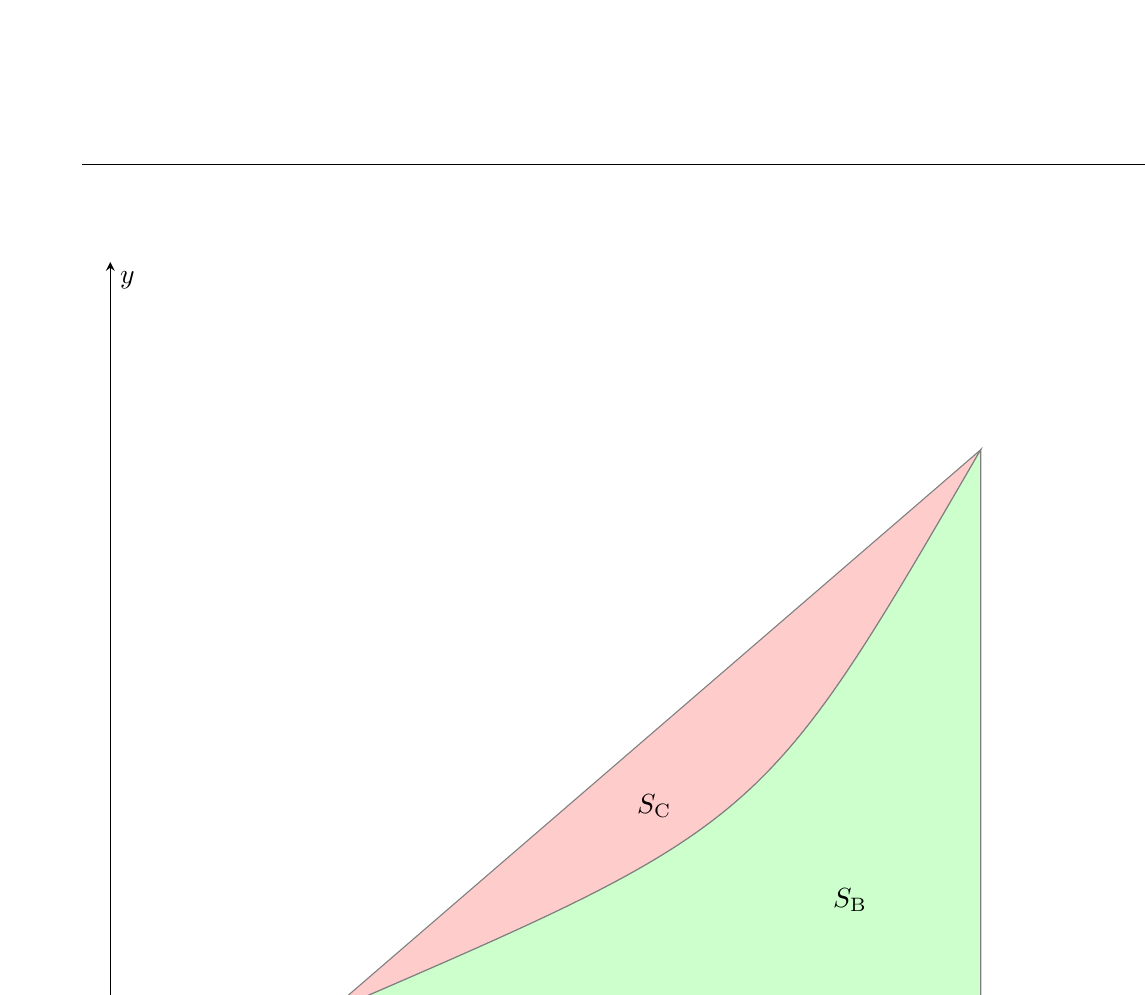
\begin{tikzpicture}
        \begin{axis}[
                ticks=none,
                axis x line=middle,
                axis y line=middle,
                xmin=0, xmax=2.5,
                ymin=0, ymax=2.5,
                xlabel=$x$,
                ylabel=$y$,
                scale only axis,
                width=\textwidth
            ]
            \coordinate (A) at (0.5, 0);
            \coordinate (B) at (0.5, 0.5);
            \coordinate (C) at (2, 2);
            \coordinate (D) at (2, 0.5);
            \coordinate (E) at (2, 0);
            \draw [Gray,fill=red!20!white] (B) .. controls (1.5, 1) .. (C) --cycle;
            \draw [Gray,fill=green!20!white] (B) .. controls (1.5, 1) .. (C) -- (D) -- cycle;
            \draw [Gray,fill=blue!20!white] (A) -- (B) -- (D) -- (E) --cycle;
            \node [Black] at (1.25, 0.25) {$S_\mathrm{A}$};
            \node [Black] at (1.7, 0.8) {$S_\mathrm{B}$};
            \node [Black] at (1.25, 1.05) {$S_\mathrm{C}$};
        \end{axis}
    \end{tikzpicture}
    \caption{$S_\mathrm{A} < S_\mathrm{A}+S_\mathrm{B} < S_\text{A}+S_\mathrm{B}+S_\mathrm{C} $}
\end{marginfigure}
\begin{proof}
    因为$f(x)$单调增,所以$f'(x)\geq 0$,又因为$f''(x)>0$,所以$f'(x)$单调增,故$f'(x)$不恒为零,所以$f(x)$不恒为$f(a)$。
    \[ \int_a^bf(x)\dd{x} > \int_a^b f(a)\dd{x} =(b-a)f(a) \]
    所以不等式左侧成立,下证不等式右侧

    因为$f''(x)>0$,所以$f(x)$为凹函数,故有
    \[ f(x) < \frac{f(b)-f(a)}{b-a}(x-a) + f(a) \]
    因此
    \[
        \int_a^bf(x)\dd{x}
        <
        \int_a^b \frac{f(b)-f(a)}{b-a}(x-a) + f(a) \dd{x}
        =
        (b-a)\cdot\frac{f(a)+f(b)}{2}
    \]
\end{proof}

\begin{example}
    设$\displaystyle f(x) = \ln x - x\int_1^\mathrm{e}\frac{f(x)}{x}\dd{x}$,
    求$f(x)$
\end{example}
\begin{solution}
    \[
        \frac{f(x)}{x} = \frac{\ln x}{x} - \int_1^\mathrm{e}\frac{f(x)}{x}\dd{x}
        =
        \frac{\ln x}{x} - A
    \]
    两边同时在$[1,\mathrm{e}]$上积分,
    \[
        A
        =
        \int_1^\mathrm{e}\frac{f(x)}{x}\dd{x}
        =
        \int_1^\mathrm{e}\frac{\ln x}{x}\dd{x} - \int_1^\mathrm{e} A\dd{x}
        =
        \frac{1}{2} - A(\mathrm{e}-1)
    \]
    所以$A = \dfrac{1}{2\mathrm{e}}$,带入原式得
    \[ f(x) = \ln x - \frac{x}{2\mathrm{e}} \]
\end{solution}

\begin{example}
    设$\displaystyle F(x) = \int_x^{x+2\pi} \mathrm{e}^{\sin t}\sin t\dd{t}$,
    证明:$F(x)$恒为正常数。
\end{example}

\begin{proof}
    设$f(x)= \mathrm{e}^{\sin x}\sin x$,显然$f(x+2\pi) = f(x)$,则$f(x)$是以$2\pi$为周期的连续函数。
    故
    \begin{align*}
        F(x) & = \int_0^{2\pi} \mathrm{e}^{\sin t}\sin t\dd{t}                                                  \\
             & = \int_0^{\pi}\mathrm{e}^{\sin t}\sin t\dd{t} + \int_{\pi}^{2\pi}\mathrm{e}^{\sin t}\sin t\dd{t} \\
             & = \int_0^{\pi}\mathrm{e}^{\sin t}\sin t\dd{t} - \int_0^{\pi}\mathrm{e}^{-\sin t}\sin t\dd{t}     \\
             & = \int_0^{\pi}\left(\mathrm{e}^{\sin t} - \mathrm{e}^{-\sin t}\right)\sin t\dd{t}                \\
    \end{align*}
    因为在$[0,\pi]$上$\sin x > 0$,所以$\left(\mathrm{e}^{\sin x} - \mathrm{e}^{-\sin x}\right)\sin x >0$,
    故$F(x)$恒为正常数。
\end{proof}

\begin{example}
    设$f(x)$在$[a,b]$上二阶连续可微,且$\displaystyle f\left(\frac{a+b}{2}\right)=0$,证明
    \[ \abs{\int_a^bf(x)\dd{x}} \leq \frac{M}{24}(b-a)^3  \]
    其中$M=\max_{a\leq x \leq b}\abs{f''(x)}$
\end{example}
\begin{proof}
    由题意根据泰勒公式得,其中$t=\dfrac{a+b}{2},\xi $在$t$的去心领域内
    \[
        f(x)  = f(t) + f'(t)(x-t)+ \frac{1}{2}f''(\xi)(x-t)^2
        = f'(t)(x-t) + \frac{1}{2}f''(\xi)(x-t)^2
    \]
    左右绝对积分得
    \begin{align*}
        \abs{\int_a^bf(x)\dd{x}}
         & = \abs{\int_a^bf'(t)(x-t) + \frac{1}{2}f''(\xi)(x-t)^2\dd{x}}                          \\
         & \leq \abs{\int_a^b f'(t)(x-t)\dd{x}} + \abs{\int_a^b \frac{1}{2}f''(\xi)(x-t)^2\dd{x}} \\
         & = 0 + \frac{1}{2}\abs{\int_a^b f''(\xi)(x-t)^2\dd{x}}                                  \\
         & \leq \frac{M}{2}\int_a^b (x-t)^2\dd{x}                                                 \\
         & =\frac{M}{6}[(b-t)^3 - (a-t)^3]                                                        \\
         & =\frac{M}{24}(b-a)^3
    \end{align*}
\end{proof}
解此题首先要将已知的条件往结论的形式上凑。这里有一个难点是,将一个定积分拆成两个定积分,任意其中一个定积分进行变量代换时,对另一个定积分无影响。
同时积分函数相同,且上下限能合并,那么无论积分微元是$t$还是$x$,都可以合并。对于上下限相同,函数合并,是同理的。
其本质是
\[
    \int_a^b f(x)\dd{x} + \int_b^c f(x)\dd{t}
    =
    \sum_{i=n_1}^{n_2-1} a_i + \sum_{i=n_2}^{n_3-1} a_i
    =
    \sum_{i=n_1}^{n_3} a_i = \int_a^c f(x)\dd{x}
\]
\[
    \int_a^b f(x)\dd{x} + \int_a^b g(t)\dd{t}
    =
    \sum a_i + \sum b_i = \sum (a_i + b_i)
    =
    \int_a^b f(x)+g(x)\dd{x}
\]
\begin{example}
    设$f(x)$在$[0,+\infty)$上连续,$0<a<b$,且$\displaystyle\int_A^{+\infty}\frac{f(x)}{x}\dd{x}$收敛,其中常数$A>0$,证明
    \[
        \int_0^{+\infty}\frac{f(ax)-f(bx)}{x}\dd{x} = f(0)\ln\frac{b}{a}
    \]
\end{example}
\begin{proof}
    因为
    \[ \int_A^{+\infty}\frac{f(x)}{x}\dd{x} = \int_{A/a}^{+\infty} \frac{f(ax)}{x}\dd{x} \]
    \[ \int_A^{+\infty}\frac{f(x)}{x}\dd{x} = \int_{A/b}^{+\infty} \frac{f(bx)}{x}\dd{x} \]
    那么有
    \begin{align*}
        \int_\varepsilon^{+\infty} \frac{f(ax)-f(bx)}{x}\dd{x}
         & = \int_\varepsilon^{+\infty} \frac{f(ax)}{x}\dd{x} - \int_\varepsilon^{+\infty}\frac{f(bx)}{x}\dd{x}     \\
         & = \int_{a\varepsilon}^{+\infty} \frac{f(t)}{t}\dd{t} - \int_{b\varepsilon}^{+\infty}\frac{f(t)}{t}\dd{t} \\
         & = \int_{a\varepsilon}^{b\varepsilon} \frac{f(x)}{x}\dd{x}                                                \\
         & = f(\xi)\int_{a\varepsilon}^{b\varepsilon} \dd{\ln x} \qquad \xi\in(a\varepsilon,b\varepsilon)           \\
         & = f(\xi)\ln\frac{b}{a} \qquad                                                                            \\
    \end{align*}
    那么当$\xi\to 0^+$时,则有$f(\xi)=f(0)$,所以
    \[
        \int_0^{+\infty}\frac{f(ax)-f(bx)}{x}\dd{x} = f(0)\ln\frac{b}{a}
    \]
\end{proof}

\begin{example}
    设函数$f'(x)$在$[a,b]$上连续,且$f(a)=0$,证明
    \[ \int_a^b f^2(x)\dd{x} \leq \frac{(b-a)^2}{2}\int_a^b[f'(x)]^2\dd{x} \]
\end{example}
\begin{proof}
    由命题的形式可以联想到柯西不等式\ref{eq:柯西不等式},所以我们尽量往柯西不等式凑。
    \[
        \left(\int_a^x f'(t)\dd{t}\right)^2
        \leq
        \left(\int_a^x [f'(t)]^2\dd{t}\right)\cdot\left(\int_a^x 1^2\dd{t}\right)
        =
        (x-a)\int_a^x [f'(t)]^2\dd{t}
    \]
    而
    \[ \left(\int_a^x f'(t)\dd{t}\right)^2 = \left(f(x)-f(a)\right)^2 = f^2(x) \]
    所以有
    \[ 0 \leq f^2(x) \leq (x-a)\int_a^x [f'(t)]^2\dd{t} \]
    左右同时积分可得
    \begin{align*}
        \int_a^b f^2(x)\dd{x}
         & \leq
        \int_a^b (x-a)\int_a^x [f'(t)]^2\dd{t}\dd{x}  \\
         & \leq
        \int_a^b (x-a)\int_a^b [f'(t)]^2\dd{t}\dd{x}  \\
         & =
        \int_a^b (x-a)\dd{x} \int_a^b [f'(t)]^2\dd{t} \\
         & =
        \frac{(b-a)^2}{2} \int_a^b [f'(x)]^2\dd{x}
    \end{align*}
\end{proof}
上述证明中的难点是对于$f^2(x)\geq 0$,则子区间的定积分(或变限积分)小于原区间的定积分,同时定积分是一个数,
可以从双重积分中提出,再变换积分微元,此做法的本质如下
\[ \sum \left(a_i\sum b_j\right) = a_1\sum b_j + a_2\sum b_j + \cdots a_n\sum b_j = \sum a_i\cdot\sum b_j = \sum a_i\cdot\sum b_i \]

利用单调性的解法如下
\begin{proof}
    设
    \[ F(x) = \int_a^xf^2(t)\dd{t} - \frac{(x-a)^2}{2}\int_a^x[f'(t)]^2\dd{t} \]
    那么$F(a)=0$,同时
    \begin{align*}
        F'(x)
         & = f^2(x) - (x-a)\int_a^x[f'(t)]^2\dd{t} - \frac{(x-a)^2}{2}[f'(x)]^2              \\
         & = f^2(x) - \int_a^x 1^2\dd{x}\int_a^x[f'(t)]^2\dd{t} - \frac{(x-a)^2}{2}[f'(x)]^2 \\
         & \leq f^2(x) - \left(\int_a^xf'(t)\dd{t}\right)^2 - \frac{(x-a)^2}{2}[f'(x)]^2     \\
         & =f^2(x) - (f(x)-f(a))^2 - \frac{(x-a)^2}{2}[f'(x)]^2                              \\
         & =- \frac{(x-a)^2}{2}[f'(x)]^2                                                     \\
         & \leq 0
    \end{align*}
    所以$F(x)$单调递减,则$F(b) \leq F(a) = 0$,即
    \[ \int_a^b f^2(x)\dd{x} \leq \frac{(b-a)^2}{2}\int_a^b[f'(x)]^2\dd{x} \]
\end{proof}

\subsection{面积、体积计算}
\subsubsection{\texorpdfstring{$x$}{x}型区域的面积}
由上下两条曲线$y_\text{上}=f(x),y_\text{下}=g(x)$以及左右两条直线$x=a,x=b$所围成的区域面积
\[ S = \int_a^b [f(x)-g(x)]\dd{x} \]

\subsubsection{\texorpdfstring{$y$}{x}型区域的面积}
与$x$型区域的面积类似,由左右两条曲线围成$x_\text{左}=\psi(y),x_\text{右}=\varphi(y)$以及上下两条直线$y=d,y=c$所围成的区域面积
\[ S = \int_c^d [\varphi(y)-\psi(y)]\dd{y} \]

\subsubsection{参数型区域的面积}
如果曲边梯形的上边界由参数方程$x=x(t),y=y(t)\ (\alpha<t<\beta)$所确定,则有
\[ S = \int_\alpha^\beta y(t)\dd{x}(t) \]

\subsubsection{极坐标型区域的面积}
若极坐标曲线$r=f(\theta)$是连续的,那么由$r=f(\theta)$和射线$\theta=\alpha,\theta=\beta$所围成的扇形面积为
\[ S = \frac{1}{2}\int_\alpha^\beta f^2(\theta)\dd{\theta} \]

\subsubsection{几何体体积的截面算法}
如果一个集合体在$x$轴的正投影区间为$[a,b]$,并且在每一点$x\in[a,b]$的横截面积为$S(x)$,
那么当$S(x)$在$[a,b]$上连续时,该集合体体积为
\[ V = \int_a^b S(x)\dd{x} \]

\subsubsection{旋转体体积的柱形算法}
如果选旋转体是由在区间$[a,b]$上的连续曲线$y=f(x)$绕$x$轴旋转一周所形成,那么其体积为
\[ V = \pi\int_a^bf^2(x)\dd{x} \]

当所求旋转体是由两条曲线$y_1=f(x),y_2=g(x)$所夹区域,绕$x$轴旋转一周形成,且$\abs{f(x)} > \abs{g(x)}$恒成立,那么体积为
\[ V = V_1 - V_2 = \pi\int_a^b f^2(x)-g^2(x)\dd{x} \]

\subsubsection{旋转体体积的管形算法}
如果选择题由曲边梯形
\[ 0\leq y \leq f(x), a\leq x \leq b \]
绕$y$轴生成那么其体积微元为
\[ \Delta V = \pi(x+\Delta x)^2y - \pi x^2y = 2\pi xy\Delta x + \pi y\Delta x^2  \]
取线性主部积分,那么体积为
\[ V = 2\pi\int_a^bxf(x)\dd{x} \]

\subsubsection{显式曲线的弧长}
如果曲线$L$是由连续可微函数$y=f(x),x\in[a,b]$给出,则$L$是可求长曲线,
则弧长微元为
\[ \Delta s = \sqrt{\Delta x^2 + \Delta y^2} = \sqrt{1+\left(\frac{\Delta y}{\Delta x}\right)^2}\cdot \Delta x \]
因此弧长公式为
\[ s = \int_a^b \sqrt{1+[f'(x)]^2}\dd{x} \]

\subsubsection{参数曲线弧长}如果$L: x=x(t), y=y(t),t\in[a,b]$是一条不自交的连续可微曲线,则有
\[ s = \int_a^b\sqrt{x'^2+y'^2}\dd{t} \]

\subsubsection{极坐标曲线的弧长}
如果连续可微的曲线的极坐标方程为$r=r(\theta),\theta\in[\alpha,\beta]$则其参数方程为
\[ x = r(\theta)\cos\theta,y=r(\theta)\sin\theta,\theta\in[\alpha,\beta] \]
根据参数曲线的弧长公式可知
\[ s = \int_\alpha^\beta \sqrt{r^2+r'^2}\dd{\theta} \]

\section{不定积分}
定积分的计算可以寻找原函数后,再通过Newton-Leibniz公式\ref{th:Newton-Leibniz公式}计算,因此研究原函数就是不定积分的计算
\begin{definition}
    设函数$f(x)$是$[a,b]$上的连续函数,则面积函数
    \[ F(x) = \int_a^x f(t)\dd{t} \]
    是$[a,b]$上的可导函数,且$F'(x)=f(x)$
\end{definition}
\begin{definition}
    如果在区间$I$上,可导函数$F(x)$的导函数为$f(x)$,即当$x\in I$时,恒有
    \[ F'(x) = f(x) \]
    则称$F(x)$时$f(x)$在区间$I$上的一个原函数。
    注:连续函数的面积函数是其中一个原函数。
\end{definition}
\begin{definition}
    函数$f(x)$在区间$[a,b]$上的全体原函数成为$f(x)$再$[a,b]$上的不定积分,记作$\int f(x)\dd{x}$

    如果$F(x)$是函数$f(x)$再区间$[a,b]$上的一个原函数,则有
    \[\int f(x)\dd{x} = \left\{F(x)+C \,\middle|\, C\in\mathbf{R} \right\} \]
\end{definition}

在原函数的定义中可知,原函数一定可导,所以原函数一定连续,(原函数的导函数在区间\textcolor{red}{可以不连续}(看下题的注释),但在区间的每个都有定义,即导函数有值)。
\begin{example}
    证明:含第一类间断点、无穷型第二类间断点的函数$f(x)$在包含该间断点的区间内没有原函数$F(x)$
\end{example}
\begin{proof}
    假设$F(x)$为$f(x)$的原函数,那么有$F'(x)=f(x)$,设$x=x_0$为间断点,由题意可知$f(x_0)$有定义,
    在下面分类讨论
    \begin{enumerate}[(1)]
        \item 当$x=x_0$为第一类可去间断点时,即$\lim_{x\to x_0} f(x) \neq f(x_0)$,则有
              \begin{align*}
                  f(x_0) = F'(x_0) & = \lim_{x\to x_0}\frac{F(x)-F(x_0)}{x-x_0}     \\
                                   & =\lim_{x\to x_0}F'(x) \qquad \text{洛必达法则} \\
                                   & = \lim_{x\to x_0} f(x)
              \end{align*}
              矛盾,所以$F(x)$不存在。
        \item 当$x=x_0$为第一类跳跃间断点时,不妨令$\lim_{x\to x^-} f(x) \neq \lim_{x\to x^+}$
              \begin{align*}
                  f(x_0) = F'(x_0) & = \lim_{x\to x_0}\frac{F(x)-F(x_0)}{x-x_0}     \\
                                   & =\lim_{x\to x_0}F'(x) \qquad \text{洛必达法则} \\
                                   & = \lim_{x\to x_0} f(x)
              \end{align*}
              由于$f(x_0)$存在,但$\lim_{x\to x_0} f(x)$不存在,矛盾,所以$F(x)$不存在。
        \item 无穷型第二类间断点的函数与(2)同理可证。
    \end{enumerate}
    注:非无穷型的第二类间断点(非无穷振荡点)的函数,可以有原函数,因具体分析,如
    \[
        F(x)=
        \begin{cases}
            x^2\sin\frac{1}{x}, & x\neq 0, \\
            0,                  & x=0
        \end{cases}
    \]
    是
    \[
        f(x)=
        \begin{cases}
            2x\sin\frac{1}{x} - \cos\frac{1}{x}, & x\neq 0, \\
            0,                                   & x=0
        \end{cases}
    \]
    的原函数。
    而
    \[
        f(x)=
        \begin{cases}
            \sin\frac{1}{x}, & x\neq 0, \\
            0,               & x=0
        \end{cases}
    \]
    不存在原函数。
\end{proof}

\subsection{积分方法}
\subsubsection{换元积分法}
大多数的积分需要通过变量代换化简后计算,也称换元积分法
\begin{theorem}
    (第一类换元法)
    设函数$f(u)$存在原函数,$u=\varphi(x)$可导,则
    \[ \int f\circ\varphi(x)\cdot \varphi'(x)\dd{x} = \eval{\int f(u)\dd{u}}_{u=\varphi(x)} \]
    若函数$u=\varphi(x)$在区间$I=[a,b]$上连续可导,
    函数$f(u)$在区间$\varphi(I)=\left\{\varphi(x) \,\middle|\, x\in[a,b]\right\}$上连续,
    若$\alpha=\varphi(a),\beta=\varphi(b)$,则
    \[
        \int_a^b f\circ\varphi(x)\cdot\varphi'(x)\dd{x}
        =
        \int_{\varphi(a)}^{\varphi(b)} f(u)\dd{u}
        =
        \int_\alpha^\beta f(u)\dd{u}
    \]
\end{theorem}

\begin{example}
    求$\displaystyle\int \frac{1}{\sin^2 x + 2\cos^2 x}\dd{x}$
\end{example}
\begin{solution}
    \begin{align*}
        \int \frac{1}{\sin^2 x + 2\cos^2 x}\dd{x}
         & = \int \frac{1}{\tan^2 x + 2}\frac{\dd{x}}{\cos^2 x}            \\
         & = \int \frac{1}{\tan^2 x + (\sqrt{2})^2} \dd{\tan x}            \\
         & = \frac{1}{\sqrt{2}}\arctan\left(\frac{\tan x}{\sqrt{2}}\right)
    \end{align*}
\end{solution}


\begin{theorem}
    (第二类换元法)
    设$x=\varphi(t)$在区间$I$上连续可导且$\varphi'(t)\neq 0$,若$f(x)$在区间$\varphi(I)$上存在原函数,则
    \[ \int f(x)\dd{x} = \eval{\int f\circ\varphi(t)\cdot\varphi'(t)\dd{t}}_{t=\varphi^{-1}(x)} \]
\end{theorem}
\begin{situation}
    第二类换元法是第一类换元法的反向使用,也称“拆微分”。当被积函数中部分项比较复杂,或存在三角代换、双曲代换时,可使用此方法。
\end{situation}

\subsubsection{分部积分法}
由于$(uv)'=u'v+uv'$,所以有
\begin{theorem}
    (分部积分法)
    设$u=u(x),v=v(x)$是区间$[a,b]$上的连续可导函数,则
    \[ \int u\dd{v} = uv - \int v\dd{u} \qquad \int_a^b u\dd{v} = \eval{uv}_a^b - \int_a^bv\dd{u} \]
\end{theorem}
\begin{situation}
    分部积分法适用于含$\mathrm{e}^x,\ln x$和三角函数的积分,因为其多次求导具有周期的性质,或可以与某些项相消,故多次使用分部积分法后移项,即可求出积分。
    \begin{alignat*}{43}
         & \int P_n(x)\mathrm{e}^{kx}\dd{x}     & = &   & \frac{1}{k} & \int P_n(x)\dd{\mathrm{e}^kx)}      \\
         & \int P_n(x)\sin ax\dd{x}             & = & - & \frac{1}{a} & \int P_n(x)\dd{\cos ax}             \\
         & \int P_n(x)\cos ax\dd{x}             & = &   & \frac{1}{a} & \int P_n(x)\dd{\sin ax}             \\
         & \int \mathrm{e}^{kx}\sin(ax+b)\dd{x} & = & - & \frac{1}{a} & \int \mathrm{e}^{kx}\dd{\cos(ax+b)} \\
         & \int \mathrm{e}^{kx}\cos(ax+b)\dd{x} & = &   & \frac{1}{a} & \int \mathrm{e}^{kx}\dd{\sin(ax+b)} \\
         & \int P_n'(x)\ln x\dd{x}              & = &   &             & \int \ln x\dd{P_n(x)}               \\
         & \int P_n'(x)\arcsin x\dd{x}          & = &   &             & \int \arcsin x\dd{P_n(x)}           \\
         & \int P_n'(x)\arccos x\dd{x}          & = &   &             & \int \arccos x\dd{P_n(x)}
    \end{alignat*}

    其中$P_n(x)$为$n$次多项式,$k,a,b$为常数
\end{situation}
利用分部积分法,还可以建立一些不定积分的递推公式
\begin{example}
    求$I_n=\int \sin^n x\dd{x}$
\end{example}
\begin{solution}
    \begin{align*}
        I_n & = \int \sin^{n-1} x \dd(-\cos x)                                            \\
            & = -\cos x\sin^{n-1}x + \int \cos x\cdot(n-1)\sin^{n-2}x\cos x\dd{x}         \\
            & = -\cos x\sin^{n-1}x + (n-1)\int (1-\cos^2 x)\sin^{n-2}x\dd{x}              \\
            & = -\cos x\sin^{n-1}x + (n-1)\int \sin^{n-2}x\dd{x} - (n-1)\int\sin^nx\dd{x} \\
            & = -\cos x\sin^{n-1}x + (n-1)I_{n-2} - (n-1)I_n
    \end{align*}
    所以
    \[ I_n = -\frac{1}{n}\cos x\sin^{n-1}x + \frac{n-1}{n}I_{n-2} \]
\end{solution}

\subsubsection{三角乘积的积分}
在含三角乘积的积分中,常用到半角公式
\[ \cos^2x = \frac{1+\cos 2x}{2}, \qquad \sin^2 x = \frac{1-\cos 2x}{2} \]
与积化和差公式
\begin{align*}
    \sin\alpha\cos\beta & = \frac{1}{2}[\sin(\alpha+\beta)+\sin(\alpha-\beta)] \\
    \sin\alpha\sin\beta & = \frac{1}{2}[\cos(\alpha-\beta)-\cos(\alpha+\beta)] \\
    \cos\alpha\cos\beta & = \frac{1}{2}[\cos(\alpha+\beta)+\cos(\alpha-\beta)]
\end{align*}

\begin{example}
    求$\displaystyle \int\sin 3x\sin 2x\dd{x}$
\end{example}
\begin{solution}
    \[
        \int\sin 3x\sin 2x\dd{x}
        =
        \frac{1}{2}\int [\cos(3x-2x) - \cos(3x+2x)] \dd{x}
        =
        \frac{1}{2}\sin x - \frac{1}{10}\sin 5x + C
    \]
\end{solution}
\begin{example}
    求$\displaystyle \int(1+\cos 3x)^{3/2}\dd{x}$
\end{example}
\begin{solution}
    利用半角公式有
    \begin{align*}
        \int(1+\cos 3x)^{3/2}\dd{x} & = 2\sqrt{2}\int \cos[3](\frac{3x}{2})\dd{x}                                            \\
                                    & = \frac{4\sqrt{2}}{3}\int \left[1-\sin[2](\frac{3x}{2})\right]\dd{\sin(\frac{3x}{2})}  \\
                                    & = \frac{4\sqrt{2}}{3}\sin(\frac{3x}{2}) - \frac{4\sqrt{2}}{9}\sin[3](\frac{3x}{2}) + C \\
                                    & = \frac{4\sqrt{2}}{9}\left[3\sin(\frac{3x}{2})-\sin[3](\frac{3x}{2})\right] + C
    \end{align*}
\end{solution}

\subsubsection{万能公式求解三角函数积分}
若被积函数为含三角函数的分式时,且不好“凑微分”、化简时,可以利用三角函数的万能公式将其转化为有理分式的积分。
\begin{align}
    \label{eq:万能公式}
    \sin x & = \frac{2t}{1+t^2}    \\
    \cos x & = \frac{1-t^2}{1+t^2} \\
    \tan x & = \frac{2t}{1-t^2}
\end{align}
其中$t=\tan \frac{x}{2}$。

其本质是三角函数的降角升幂,同时提取$\sec^2\frac{x}{2}$,使得不定积分变为
\[ \int f(x)\dd{x} = 2\int \sec^2\frac{x}{2}\cdot g\left(\tan\frac{x}{2}\right) \dd{\frac{x}{2}} = 2\int g\left(\tan\frac{x}{2}\right)\dd{\tan\frac{x}{2}} \]

\begin{example}
    求$\displaystyle\int\frac{\dd{x}}{2+\sin x}$
\end{example}
\begin{solution}
    \begin{align*}
        \int\frac{\dd{x}}{2+\sin x}
         & = \int\frac{\dd{x}}{2+2\sin\frac{x}{2} \cos\frac{x}{2}}                                                              \\
         & = \int\frac{1}{\sin^2\frac{x}{2} + \cos^2\frac{x}{2} + \sin\frac{x}{2} \cos\frac{x}{2}}\dd{\frac{x}{2}}              \\
         & = \int\sec^2\frac{x}{2} \cdot \frac{1}{\tan^2\frac{x}{2} + 1 + \tan\frac{x}{2}} \dd{\frac{x}{2}}                     \\
         & = \int\frac{1}{\left(\tan\frac{x}{2} + \frac{1}{2}\right)^2 + \left(\frac{\sqrt{3}}{2}\right)^2}\dd{\tan\frac{x}{2}} \\
         & = \frac{2}{\sqrt{3}}\arctan\left(\frac{2\tan\frac{x}{2}+1}{\sqrt{3}}\right) + C
    \end{align*}
\end{solution}

\subsubsection{有理函数的积分(有理分式的积分)}
设多项式
\begin{align*}
    P(x) & = a_0x^n + a_1x^{n-1} + \cdots + a_{n-1}x + a_n, & (a_0\neq 0) \\
    Q(x) & = b_0x^m + b_1x^{m-1} + \cdots + b_{m-1}x + b_m, & (b_0\neq 0) \\
\end{align*}
使得$R(x)=\dfrac{P(x)}{Q(x)}$,其中$P(x),Q(x)$之间无公因式,
当$m>n$时,$R(x)$为真分式,当$m\leq n$时,$R(x)$为假分式,假分式可分解为一个多项式与一个真分式的和,如
\[ \frac{x^4 + x^2 + x + 1}{x^2 + 1} = x^2 + \frac{x + 1}{x^2 + 1} \]
故以下只研究真分式$R(x)$即可。

对真分式$R(x)$进行积分,通常需要以下几个步骤
\begin{enumerate}[(1)]
    \item 因式分解真分式$R(x)=\dfrac{P(x)}{Q(x)}$中的$Q(x)$
    \item 根据$Q(x)$的因式分解结果,构造待定系数的$R(x)$
    \item 计算待定系数,得出$R(x)$的部分分式型
    \item 对每一项部分分式进行积分
\end{enumerate}

\paragraph{有理函数的分解}
形如
\begin{tasks}[label=(\arabic*),label-width = 2em](2)
    \task $\dfrac{A}{x-a}$
    \task $\dfrac{A}{(x-a)^n}$
    \task $\dfrac{Mx+N}{x^2+px+q}$
    \task $\dfrac{Mx+N}{(x^2+px+q)^n}$
\end{tasks}
的函数称为\textsf{\textbf{部分分式}},其中$A,M,N$为常数,$p^2-4q<0,n\geq 2$

在真分式$R(x)=\dfrac{P(x)}{Q(x)}$中,当$Q(x)$存在因式分解:
\[ Q(x) = (x-a)^k\varphi(x) \]
则有
\[ R(x) = \frac{A_1}{x-a} + \frac{A_2}{(x-a)^2} + \cdots + \frac{A_k}{(x-a)^k} + \frac{\psi(x)}{\varphi(x)} \]
当$Q(x)$存在因式分解:
\[ Q(x) = (x^2+px+q)^k\varphi(x),p^2-4q<0 \]
则有
\[ R(x) = \frac{M_1x+N_1}{x^2+px+q} + \frac{M_2x+N_2}{(x^2+px+q)^2} + \cdots + \frac{M_kx+N_k}{(x^2+px+q)^k} + \frac{\psi(x)}{\varphi(x)} \]
其中$\dfrac{\psi(x)}{\varphi(x)}$为真分式,$A_1,M_1,N_1,\cdots,A_k,M_k,N_k$为待定系数。

若$Q(x)\neq 0$恒成立,无论其阶数多高,总能分解为(3),(4)两种部分分式。
\begin{example}
    因式分解$Q(x) =x^4+1$
\end{example}
\begin{solution}
    \[ Q(x) = x^4+1 = (x^2+1)^2-2x^2 = (x^2-\sqrt{2}x+1)(x^2+\sqrt{2}x+1) \]
\end{solution}

\paragraph{待定系数的计算}
常用方法有通分法,特值法,极限法,也可以综合使用。由于通分法需要解方程组,当待定系数过多时,计算复杂且容易出错。
下面给出两个实际的例子说明
\begin{example}
    设
    \[ R(x) = \frac{1}{(1+2x)(1+x^2)} \]
    分解$R(x)$为部分分式的和。
\end{example}
\begin{solution}
    用通分法。令
    \[ R(x) = \frac{1}{(1+2x)(1+x^2)} = \frac{A}{1+2x} + \frac{Bx+C}{1+x^2} \]
    通分得出分子等式
    \[ (A+2B)x^2 + (B+2C)x + 1 = 1 \]
    对应系数相等可得三元一次方程组
    \[
        \begin{cases}
            A+2B = 0 \\
            B+2C = 0 \\
            A+C  = 1
        \end{cases}
    \]
    解得$A=\dfrac{4}{5},B=-\dfrac{2}{5},C=\dfrac{1}{5}$,所以
    \[ R(x) = \frac{4}{5(1+2x)} + \frac{-2x + 1}{5(1+x^2)} \]
\end{solution}

\begin{example}
    设
    \[ R(x) = \frac{x^3+2x^2+1}{(x-1)(x-2)(x-3)^2} \]
    分解$R(x)$为部分分式的和。
\end{example}
\begin{solution}
    用极限与特值法,令
    \[ R(x) = \frac{x^3+2x^2+1}{(x-1)(x-2)(x-3)^2} = \frac{A}{x-1} + \frac{B}{x-2} + \frac{C}{x-3} + \frac{D}{(x-3)^2} \]
    则
    \[ A = \lim_{x\to 1}R(x)(x-1) = \lim_{x\to 1}\frac{x^3+2x^2+1}{(x-2)(x-3)^2} = -1 \]
    \[ B = \lim_{x\to 2}R(x)(x-2) = 17 \]
    \[ D = \lim_{x\to 3}R(x)(x-3)^2 = 23 \]
    令$x=0$,得出$C=-15$,所以
    \[ R(x) = -\frac{1}{x-1} + \frac{17}{x-2} - \frac{15}{x-3} + \frac{23}{(x-3)^2} \]
\end{solution}



\paragraph{部分分式的积分}
对于(1)、(2)型的部分分式,可以直接计算其积分,
对于(3)、(4)型的部分分式,则需要通过“凑微分”的方式来进行积分
\begin{alignat*}{3}
     & \int \frac{Mx+N}{x^2+px+q}\dd{x}     & = & \frac{M}{2} \int \frac{\dd(x^2+px+q)}{x^2+px+q} + (N-p_1M)\int\frac{\dd(x+p_1)}{(x+p_1)^2+a^2}       \\
    \\
     & \int \frac{Mx+N}{(x^2+px+q)^n}\dd{x} & = & \frac{M}{2}\int\frac{\dd(x^2+px+q)}{(x^2+px+q)^n} + (N-p_1M)\int\frac{\dd(x+p_1)}{[(x+p_1)^2+a^2]^n}
\end{alignat*}
其中$p_1=\dfrac{p}{2},a=\sqrt{q-p_1^2}$

在凑出的积分中比较难计算的是$\displaystyle\int\frac{\dd(x+p_1)}{[(x+p_1)^2+a^2]^n} $即形如$\displaystyle I_n = \int\frac{\dd{x}}{(x^2+a^2)^n} $
可用分部积分法计算递推公式
\begin{align*}
    I_{n-1} & = \int\frac{\dd{x}}{(x^2+a^2)^{n-1}}                                                                              \\
            & = \frac{x}{(x^2+a^2)^{n-1}} - \int x \dd{\frac{1}{(x^2+a^2)^{n-1}}  }                                             \\
            & = \frac{x}{(x^2+a^2)^{n-1}} + 2(n-1)\int \frac{x^2}{(x^2+a^2)^n}\dd{x}                                            \\
            & = \frac{x}{(x^2+a^2)^{n-1}} + 2(n-1)\int \left[ \frac{1}{(x^2+a^2)^{n-1}} - \frac{a^2}{(x^2+a^2)^n} \right]\dd{x} \\
            & = \frac{x}{(x^2+a^2)^{n-1}} + 2(n-1)I_{n-1} - 2a^2(n-1)I_n
\end{align*}
所以
\[ I_n = \frac{1}{2a^2(n-1)}\left[ \frac{x}{(x^2+a^2)^{n-1}} + (2n-3)I_{n-1} \right] \]
根据$I_1$计算即可
\[ I_1 = \int\frac{\dd{x}}{x^2+a^2} = \frac{1}{a}\arctan \frac{x}{a} + C \]

\subsubsection{特殊无理函数的积分}
\paragraph{线商类无理式的积分}
由无理函数$u=\sqrt[n]{\dfrac{ax+b}{cx+d}}$与二元有理函数$R(x,u)$构成的复合函数的积分可以通过\textcolor{red}{\textbf{\textsf{开方代换}}}转化为有理函数的积分。
\[ \int R\left(x,\sqrt[n]{\frac{ax+b}{cx+d}}\right)\dd{x} = n(ad-bc)\int R\left(\frac{b-t^nd}{ct^n-a},t\right)\frac{t^n-1}{(ct^n-a)^2}\dd{t} \]
其中$n$为$R(x)$中$\sqrt[a_1]{\dfrac{ax+b}{cx+d}},\sqrt[a_2]{\dfrac{ax+b}{cx+d}},\cdots$的$a_1,a_2,\cdots$的最小公倍数。
\begin{example}
    求$\displaystyle\int\frac{x^{1/7}+x^{1/2}}{x^{8/7}+x^{15/14}}\dd{x}$
\end{example}
\begin{solution}
    由于指数分母的最小公倍数为$14$,故令$t=\sqrt[14]{x}$,
    \begin{align*}
        \int\frac{x^{1/7}+x^{1/2}}{x^{8/7}+x^{15/14}}\dd{x} & = 14\int(t^4-t^3+t^2-t+1)\dd{t}                                                                        \\
                                                      & =14(\frac{1}{5}x^{5/14} - \frac{1}{4}x^{2/7} + \frac{1}{3}x^{3/14} - \frac{1}{2}x^{1/7} + x^{1/14}) +C
    \end{align*}
\end{solution}

\paragraph{二次无理式的积分}
由无理函数$u=\sqrt{ax^2+bx+c}$与二元函数$R(x,u)$构成的复合函数的积分,即
\[ \int R(x,\sqrt{ax^2+bx+c})\dd{x}, (a\neq 0, b^2-4ac\neq 0) \]
则可以将$R(x,\sqrt{ax^2+bx+c})$变形为如下形式之一
\[ R^*(t, \sqrt{t^2+k^2}), R^*(t, \sqrt{t^2-k^2}), R^*(t, \sqrt{k^2-t^2}) \]
再利用\textcolor{red}{\textsf{\textbf{三角代换}}}或\textcolor{red}{\textsf{\textbf{双曲代换}}},即可进行积分。
,但有时用\textcolor{red}{\textsf{\textbf{欧拉代换}}}可能更方便。

当$a>0$时,令$\sqrt{ax^2+bx+c}=t\pm\sqrt{a}x$,称为\textcolor{red}{\textsf{\textbf{欧拉代换}}},此时
\[x=\frac{t^2-c}{b\mp\sqrt{a}t}\]
则原积分可转化为有理函数的积分。

\begin{example}
    计算$\displaystyle\int\frac{\dd{x}}{\sqrt{x^2+10x+21}}$
\end{example}
\begin{solution}
    令$x+5=2\sec t$,则
    \begin{align*}
        \int\frac{\dd{x}}{\sqrt{x^2+10x+21}} & = \int\frac{\dd(x+5)}{\sqrt{(x+5)^2-4}}        \\
                                             & = \int\frac{\dd(2\sec t)}{2\sqrt{\sec^2 t -1}} \\
                                             & = \int\frac{\dd\sec t}{\tan t}                 \\
                                             & = \int\sec t\dd{t}                             \\
                                             & = \ln\abs{\sec t+\tan t} +C                    \\
                                             & = \ln\abs{x+5+\sqrt{x^2+10x+21}} +C
    \end{align*}
\end{solution}

\begin{example}
    求$\displaystyle\int \frac{x\ln\left(x+\sqrt{1+x^2}\right)}{(1+x^2)^2}\dd{x}$
\end{example}
\begin{solution}
    由于积分中出现$1+x^2$故使用双曲代换,令$x = \sinh t$,则有$t = \ln(x+\sqrt{1+x^2})$
    \begin{align*}
        \int \frac{x\ln\left(x+\sqrt{1+x^2}\right)}{(1+x^2)^2}\dd{x}
         & = \int \frac{t\sinh t}{\cosh^4t}\dd{\sinh t}
        = \int \frac{t\sinh t}{\cosh^3t}\dd{t}
        = \int t\tanh t \dd{\tanh t}                                                 \\
         & = \frac{1}{2} \int t \dd{\tanh^2 t}
        \frac{1}{2} \left( t\tanh^2 t - \int \tanh^2 t\dd{t} \right)                 \\
         & = \frac{1}{2} \left( t\tanh^2 t - \int 1-\frac{1}{\cosh^2t}\dd{t} \right) \\
         & = \frac{1}{2} (t\tanh^2 t - t + \tanh t)+C                                \\
         & = \frac{1}{2} \left(-\frac{t}{\cosh^2 t} + \tanh t\right)+C               \\
         & =  -\frac{\ln(x+\sqrt{1+x^2})}{2(1+x^2)} + \frac{x}{2\sqrt{1+x^2}}+C      \\
    \end{align*}
\end{solution}

\subsubsection{隐函数的积分}
若方程$F(x,y)=0$确定函数$y=f(x)$,那么对于积分$\displaystyle\int m(x,y)\dd{n(x,y)}$的积分,
可以利用参数化转为一元函数的积分。
\begin{example}
    设函数$x=x(y)$由方程$x(y-x)^2=y$所确定,试求$\displaystyle\int\frac{1}{y-x}\dd{y}$
\end{example}
\begin{solution}
    令$t=y-x$,那么有$x = \dfrac{t}{t^2-1},y = \dfrac{t^3}{t^2-1}$,所以
    \begin{align*}
        \int\frac{1}{y-x}\dd{y}
         & = \int\frac{1}{t}\dd{\frac{t^3}{t^2-1}}                      \\
         & = \frac{t^2}{t^2-1} - \int \frac{t^3}{t^2-1}\dd{\frac{1}{t}} \\
         & = \frac{t^2}{t^2-1} + \int \frac{t}{t^2-1}\dd{t}             \\
         & = \frac{t^2}{t^2-1} + \frac{1}{2}\ln\abs{t^2-1} + C          \\
         & = \frac{1}{(y-x)^2-1} + \frac{1}{2}\ln\abs{(y-x)^2-1} + C    \\
    \end{align*}
\end{solution}

\section{变限积分和分段积分}
\paragraph{变限积分}

对于闭区间$[a,b]$上的连续函数$f(x)$,其面积函数为
\[ F(x) = \int_a^xf(x)\dd{x} \]
并且有$F'(x)=f(x)$,当上限与下限都为$x$的函数时,则为变限积分
\begin{theorem}
    (变限积分求导公式)
    \label{th:变限积分求导公式}
    设$\alpha(x),\beta(x)$是闭区间$[a,b]$到$[A,B]$的可导函数,若函数$f(x)$是$[A,B]$上的连续函数,则有
    “变限导数$=$上代上导$-$下代下导”,即
    \[
        \left( \int_{\alpha(x)}^{\beta(x)}f(t)\dd{t} \right)'
        =
        f(\beta)\beta'(x) - f(\alpha)\alpha'(x)
    \]
\end{theorem}
当被积函数为$f(x,t)\dd{t}$时,则需要消去$x$,一般通过换元法变为$f(u)\varphi(x,t)\dd{u}$,将$x$提出到积分外,同时调整上下限,
此时积分内部只含有$u$,再使用变限积分求导公式。
\begin{example}
    设函数$f(x)$连续,$\displaystyle\varphi(x)=\int_0^1f(xt)\dd{t}$,且$\displaystyle\lim_{x\to 0}\frac{f(x)}{x}=A$,
    求$\varphi'(x)$并讨论$\varphi'(x)$在$x=0$处的连续性。
\end{example}
\begin{solution}
    由$\displaystyle\lim_{x\to 0}\frac{f(x)}{x}=A$可知$f(0)=0$,从而$\varphi(0)=0$
    令$u=xt$,则当$x\neq 0$时,有
    \[ \varphi(x) = \frac{1}{x}\int_0^x f(u)\dd{u} ,\qquad (x\neq 0)\]
    于是
    \[
        \varphi'(x)
        =
        \frac{1}{x^2}\left(xf(x) - \int_0^xf(u)\dd{u}\right)
        = \frac{f(x)}{x} - \frac{1}{x^2}\int_0^xf(u)\dd{u},\qquad (x\neq 0)
    \]
    所以
    \[
        \varphi'(0)
        =
        \lim_{x\to 0}\frac{\varphi(x)-\varphi(0)}{x-0}
        =
        \lim_{x\to 0}\frac{1}{x^2}\int_0^x f(u)\dd{u}
        =
        \lim_{x\to 0}\frac{f(x)}{2x}
        =
        \frac{A}{2}
    \]
    \[
        \lim_{x\to 0}\varphi'(x)
        =
        \lim_{x\to 0}\left(\frac{f(x)}{x} - \frac{1}{x^2}\int_0^xf(u)\dd{u}\right)
        =
        A -  \lim_{x\to 0}\frac{1}{x^2}\int_0^x f(u)\dd{u}
        =
        \frac{A}{2}
    \]
    所以$\varphi'(x)$在$x=0$处连续
\end{solution}

\paragraph{分段积分}
\begin{enumerate}[(1)]
    \item 计算分段函数的不定积分,可以先在每个分段区间上计算不定积分,然后再讨论\textcolor{red}{被积函数}在每个\textcolor{red}{分段点}处的连续性,
          若分段点是第一类间断点、无穷型的第二类间断点,那么此点无原函数,最后再讨论原函数再分段点的连续性。
    \item 计算分段函数的定积分时,可以先计算每个分段区间上的定积分,然后对这些定积分求和。
    \item 计算复合型分段函数的定积分时,一般需要先作变量代换以化简积分表达式。
\end{enumerate}
\begin{example}
    设
    \[
        f(x) =
        \begin{cases}
            \sin x, & x<0,           \\
            x,      & 0\leq x \leq 1 \\
            2,      & x>1
        \end{cases}
    \]
    求$\displaystyle\int f(x)\dd{x}$
\end{example}
\begin{solution}
    当$x<0$时,$\displaystyle\int f(x)\dd{x} = -\cos x + C_1$

    当$0\leq x \leq 1$时,$\displaystyle\int f(x)\dd{x} = \frac{x^2}{2} + C_2$

    当$x>1$时,$\displaystyle\int f(x)\dd{x} = 2x + C_3$

    由于$f(x)$在$x=0$处连续,故存此点$f(x)$存在在原函数,那么有
    \[ \lim_{x\to 0^-} -\cos x + C_1 = \lim_{x\to 0^+} \frac{x^2}{2} + C_2 \]
    得$C_2=C_1 - 1$

    由于$f(x)$在$x=1$处不连续,故此点$f(x)$无原函数。综上可得
    \[
        \int f(x)\dd{x} =
        \begin{cases}
            -\cos x + C_1,            & x<0,           \\
            \frac{x^2}{2}  - 1 + C_1, & 0\leq x \leq 1 \\
            2x + C_3,                 & x>1
        \end{cases}
    \]
    其中$C1,C3$相互独立。
\end{solution}

\section{广义积分}
由于定积分必须保证积分区间有界、被积函数在积分区间必须有界。当去掉这两个限制时,就出现了\textcolor{red}{\textsf{\textbf{广义积分}}}。
\subsection{无穷积分}
在无穷区间上的广义积分称为\textcolor{red}{\textsf{\textbf{无穷积分}}}。
\begin{definition}
    设函数$f(x)$在区间$[a,+\infty)$有定义,如果$f(x)$在每个区间$[a,b]$上都可积,
    则称$f(x)$在$[a,+\infty)$上的无穷积分为
    \[ \int_a^{+\infty} f(x)\dd{x} = \lim_{b\to +\infty}\int_a^bf(x)\dd{x} \]
    关于无穷积分的敛散性如下
    \[ \int_a^{+\infty} f(x)\dd{x}\text{ 收敛}\iff \lim_{b\to +\infty}\int_a^bf(x)\dd{x}\text{ 存在} \]
    \[ \int_{-\infty}^b f(x)\dd{x}\text{ 收敛}\iff \lim_{a\to -\infty}\int_a^bf(x)\dd{x}\text{ 存在} \]
    \[ \int_{-\infty}^{+\infty} f(x)\dd{x}\text{ 收敛} \iff  \int_a^{+\infty} f(x)\dd{x}\text{ 与 }\int_{-\infty}^a f(x)\dd{x}\text{ 同时收敛}, \forall a\in\mathrm{R} \]
\end{definition}
按照不等式$0\leq f(x)\leq g(x)$,可称$\displaystyle\int_a^{+\infty}f(x)\dd{x}$为小积分,
$\displaystyle\int_a^{+\infty}g(x)\dd{x}$为大积分。要证明一个积分收敛,最基本的方法就是构造一个收敛的大积分,
要怎么一个积分发散,最基本的方法就是构造一个发散的小积分。大积分收敛时,小积分收敛;小积分发散时大积分发散。

\begin{theorem}
    (比较判别法)
    \label{th:无穷积分比较判别法}
    设函数$f(x),g(x)$时$[a,+\infty)$上的连续函数,如果$x\to+\infty$时,恒有$0\leq f(x) \leq g(x)$,则
    \begin{enumerate}[(1)]
        \item $\displaystyle\int_a^{+\infty} g(x)\dd{x}$收敛$\displaystyle\implies\int_a^{+\infty}f(x)\dd{x}$收敛;(大积分收敛小收敛)
        \item $\displaystyle\int_a^{+\infty} f(x)\dd{x}$发散$\displaystyle\implies\int_a^{+\infty}g(x)\dd{x}$发散;(小积分发散大发散)
    \end{enumerate}
\end{theorem}

\begin{theorem}
    (极限判别法)
    \label{th:无穷积分极限判别法}
    设函数$f(x),g(x)$在$[a,+\infty)$上非负连续,若$\displaystyle\lim_{x\to+\infty}\frac{f(x)}{g(x)}=l$,则
    \begin{enumerate}[(1)]
        \item 当$0<l<+\infty$时,$\displaystyle\int_a^{+\infty}f(x)\dd{x}\text{与}\int_a^{+\infty}g(x)\dd{x}$同时收敛或同时发散;
        \item 当$l=0$时,$\displaystyle\int_a^{+\infty}f(x)\dd{x}\text{ 发散}\implies\int_a^{+\infty}g(x)\dd{x}\text{ 发散}$;
        \item 当$l=+\infty$时,$\displaystyle\int_a^{+\infty}f(x)\dd{x}\text{ 收敛}\implies\int_a^{+\infty}g(x)\dd{x}\text{ 收敛}$;
    \end{enumerate}
\end{theorem}

\begin{theorem}
    (柯西判别法)
    \label{th:无穷积分柯西判别法}
    设$f(x)$在$[a,+\infty)$上非负连续,若$\displaystyle\lim_{x\to+\infty}x^pf(x)=l$,则
    \begin{enumerate}[(1)]
        \item 当$0\leq l < +\infty,p>1$时,$\displaystyle\int_a^{+\infty}f(x)\dd{x}$收敛;
        \item 当$0< l \leq +\infty,p\leq 1$时,$\displaystyle\int_a^{+\infty}f(x)\dd{x}$发散;
    \end{enumerate}
\end{theorem}

\begin{theorem}
    (绝对收敛法)
    \label{th:无穷积分绝对收敛法}
    设函数$f(x)$在$[a,+\infty)$上连续,若$\displaystyle\int_a^{+\infty}\abs{f(x)}\dd{x}$收敛,则$\displaystyle\int_a^{+\infty}f(x)\dd{x}$收敛
\end{theorem}

\subsection{瑕积分}
无界函数的广义积分称为\textcolor{red}{\textsf{\textbf{瑕积分}}}。
\begin{definition}
    设函数$f(x)$在区间$(a,b]$上有定义,如果$f(x)$在$(a,b]$的每个闭子区间都可积,且当$x\to a^+$时,$f(x)$无界,
    即$a$是$f(x)$的瑕点,则瑕积分为
    \[ \int_a^bf(x)\dd{x} = \lim_{c\to a^+}\int_c^bf(x)\dd{x} \]
    当$b$是$f(x)$的瑕点时
    \[ \int_a^b f(x)\dd{x} = \lim_{c\to b^-}\int_a^cf(x)\dd{x} \]
    当$c\in(a,b)$是$f(x)$的瑕点时
    \[ \int_a^b f(x)\dd{x} = \lim_{t\to c^-}\int_a^tf(x)\dd{x} + \lim_{t\to c^+}\int_t^bf(x)\dd{x} \]
\end{definition}

仿照无穷积分的敛散性证明,有
\begin{theorem}
    (比较判别法)
    \label{th:瑕积分比较判别法}
    设函数$f(x),g(x)$时$(a,b]$上的连续函数,如果$x\to a^+$时,恒有$0\leq f(x) \leq g(x)$,则
    \begin{enumerate}[(1)]
        \item $\displaystyle\int_a^b g(x)\dd{x}$收敛$\displaystyle\implies\int_a^bf(x)\dd{x}$收敛;(大积分收敛小收敛)
        \item $\displaystyle\int_a^b f(x)\dd{x}$发散$\displaystyle\implies\int_a^bg(x)\dd{x}$发散;(小积分发散大发散)
    \end{enumerate}
\end{theorem}

\begin{theorem}
    (极限判别法)
    \label{th:瑕积分极限判别法}
    设函数$f(x),g(x)$在$(a,b]$上非负连续,若$\displaystyle\lim_{x\to a^+}\frac{f(x)}{g(x)}=l$,则
    \begin{enumerate}[(1)]
        \item 当$0<l<+\infty$时,$\displaystyle\int_a^bf(x)\dd{x}\text{与}\int_a^bg(x)\dd{x}$同时收敛或同时发散;
        \item 当$l=0$时,$\displaystyle\int_a^bf(x)\dd{x}\text{ 发散}\implies\int_a^bg(x)\dd{x}\text{ 发散}$;
        \item 当$l=+\infty$时,$\displaystyle\int_a^bf(x)\dd{x}\text{ 收敛}\implies\int_a^bg(x)\dd{x}\text{ 收敛}$;
    \end{enumerate}
\end{theorem}

\begin{theorem}
    (柯西判别法)
    \label{th:瑕积分柯西判别法}
    设$f(x)$在$(a,b]$上非负连续,若$\displaystyle\lim_{x\to a^+}(x-a)^qf(x)=l$,则
    \begin{enumerate}[(1)]
        \item 当$0\leq l < +\infty,q<1$时,$\displaystyle\int_a^bf(x)\dd{x}$收敛;
        \item 当$0< l \leq +\infty,q\geq 1$时,$\displaystyle\int_a^bf(x)\dd{x}$发散;
    \end{enumerate}
\end{theorem}

\begin{theorem}
    (绝对收敛法)
    \label{th:瑕积分绝对收敛法}
    设函数$f(x)$在$(a,b]$上连续,若$\displaystyle\int_a^b\abs{f(x)}\dd{x}$收敛,则$\displaystyle\int_a^bf(x)\dd{x}$收敛
\end{theorem}

\subsection{\texorpdfstring{$\Gamma$-函数与$\beta$-函数}{Γ-函数与β-函数}}
广义积分
\[ \Gamma(s) = \int_0^{+\infty}x^{s-1}\mathrm{e}^{-x}\dd{x}, s> 0 \]
称为$\Gamma(s)$-函数。

当$x\to 0^+$时,$x^{s-1}\mathrm{e}^{-x} < x^{s-1}$,而$\displaystyle \int_0^\xi x^{s-1}\dd{x}$收敛,
所以$\displaystyle \int_0^\xi x^{s-1}\mathrm{e}^{-x}\dd{x}$收敛;

当$x\to+\infty$时,$x^{s-1}\mathrm{e}^{-x} < x^2\cdot x^{s-1}\mathrm{e}^{-x} \to 0$,
而$\displaystyle\lim_{x\to+\infty}\frac{x^2\cdot x^{s-1}}{\mathrm{e}^x} = 0$,
根据柯西判别法\ref{th:无穷积分柯西判别法},可知$\displaystyle \int_\xi^{+\infty} x^2\cdot x^{s-1}\mathrm{e}^{-x}\dd{x}$收敛,
所以$\displaystyle \int_\xi^{+\infty} x^{s-1}\mathrm{e}^{-x}\dd{x}$收敛;
所以广义积分$\Gamma(s)$在$s>0$的条件下,总是收敛的。

对于$\Gamma$-函数需要记住几个常用的值
\[ \Gamma(1)=1,\qquad \Gamma\left(\frac{1}{2}\right)=\sqrt{\pi},\qquad\Gamma(n+1)=n! \]
和一个递推公式
\[ \Gamma(s+1) = s\Gamma(s) \]
当$0<s<1$时,则有
\[ \Gamma(s)\Gamma(1-s) = \frac{\pi}{\sin \pi s} \]

广义积分
\[ \mathrm{B}(p,q) = \int_0^1 x^{p-1}(1-x)^{q-1}\dd{x} \qquad (p>0,q>0) \]
称为$\beta$-函数,且收敛。利用变量代换$u=1-x$可知,$\beta$-函数具有对称性,即$\mathrm{B}(p,q)=\mathrm{B}(q,p)$。
$\beta$-函数与$\Gamma$-函数的关系如下
\[ B(p,q) = \frac{\Gamma(p)\cdot\Gamma(q)}{\Gamma(p+q)} \]

利用变量代换$x=\sin^2\theta$,$\beta$-函数有等价表示
\[ \mathrm{B}(p,q) = 2\int_0^{\pi/2}\sin^{2p-1}\theta\cos^{2q-1}\theta\dd{\theta} \]
或
\[ \int_0^{\pi/2} \sin^m\theta\cos^n\theta\dd{\theta} = \frac{1}{2}\mathrm{B}(\frac{m+1}{2},\frac{n+1}{2}) \]

\begin{example}
    求$\displaystyle\int_0^2x^2\sqrt{4-x^2}\dd{x}$
\end{example}
\begin{solution}
    令$x=2\sin t$,则
    \begin{align*}
        \int_0^2x^2\sqrt{4-x^2}\dd{x} & = 16\int_0^{\pi/2} \sin^2 t\cos^2 t\dd{t}                                                                 \\
                                      & = 8 \cdot \mathrm{B}\left(\frac{3}{2},\frac{3}{2}\right)                                                  \\
                                      & = 8 \cdot \left.\Gamma\left(\frac{3}{2}\right)\cdot\Gamma\left(\frac{3}{2}\right)\middle/\Gamma(3)\right. \\
                                      & = 2 \cdot \left.\Gamma^2\left(\frac{1}{2}\right)\middle/ 2!\right.                                        \\
                                      & = \pi
    \end{align*}
\end{solution}

\subsection{广义积分的计算}
若广义积分是收敛的,那么其值可以通过极限、变量代换、中值定理等方法,以及综合运用这些方法来进行求解。
\begin{example}
    求$\displaystyle\int_0^{+\infty}\frac{\ln(\mathrm{e}x)}{1+x^2}\dd{x}$
\end{example}
\begin{solution}
    \begin{align*}
        \int_0^{+\infty}\frac{\ln(\mathrm{e}x)}{1+x^2}\dd{x}
         & = \int_0^{+\infty} \frac{1}{1+x^2}\dd{x} + \int_0^{+\infty}\frac{\ln x}{1+x^2}\dd{x}                        \\
         & = \frac{\pi}{2} + \int_0^1 \frac{\ln x}{1+x^2}\dd{x} + \int_1^{+\infty} \frac{\ln x}{1+x^2}\dd{x}           \\
         & = \frac{\pi}{2} + \int_0^1 \frac{\ln x}{1+x^2}\dd{x} + \int_1^0 \frac{\ln (1/x)}{1+(1/x)^2}\dd{\frac{1}{x}} \\
         & = \frac{\pi}{2} + \int_0^1 \frac{\ln x}{1+x^2}\dd{x} - \int_0^1 \frac{\ln x}{x^2+1}\dd{x}                   \\
         & = \frac{\pi}{2}
    \end{align*}
\end{solution}

\begin{example}
    设$f(x)$连续,且$\displaystyle\lim_{x\to+\infty} f(x) = 1$,$a$为常数,求
    $\displaystyle\lim_{x\to+\infty}\int_x^{x+a}f(t)\dd{t}$
\end{example}
\begin{solution}
    因为$f(x)$连续,故有
    \[
        \lim_{x\to+\infty}\int_x^{x+a}f(t)\dd{t}
        =
        \lim_{x\to+\infty}f(\xi)\int_x^{x+a}\dd{t}
        =
        a\lim_{x\to+\infty} f(\xi)
        =
        a
    \]
    其中$\xi\in(x,x+a)$,且$x\to+\infty$时,$\xi\to+\infty$
\end{solution}

\begin{example}
    计算$\displaystyle\lim_{x\to+\infty}\int_{x-\frac{1}{x}}^{x+\frac{1}{x}}\frac{y^{1+y}}{(1+y)^y}\dd{y}$
\end{example}
\begin{solution}
    根据积分中值定理有
    \begin{align*}
        \lim_{x\to+\infty}\int_{x-\frac{1}{x}}^{x+\frac{1}{x}}\frac{y^{1+y}}{(1+y)^y}\dd{y}
         & = \lim_{x\to+\infty} \frac{\xi^{1+\xi}}{(1+\xi)^\xi} \int_{x-\frac{1}{x}}^{x+\frac{1}{x}}\dd{y} \\
         & = \lim_{x\to+\infty} \frac{\xi^{1+\xi}}{(1+\xi)^\xi} \cdot \frac{2}{x}                          \\
    \end{align*}
    其中$\xi\in[x-\frac{1}{x},x+\frac{1}{x}]$,当$x\to+\infty$时,$\xi \sim x$,所以有
    \begin{align*}
        \lim_{x\to+\infty}\int_{x-\frac{1}{x}}^{x+\frac{1}{x}}\frac{y^{1+y}}{(1+y)^y}\dd{y}
         & = \lim_{x\to+\infty} \frac{x^{1+x}}{(1+x)^x} \cdot \frac{2}{x} \\
         & = 2\lim_{x\to+\infty} \left(\frac{x}{1+x}\right)^x             \\
         & = 2\lim_{x\to 0^+} \left(\frac{1}{1+x}\right)^\frac{1}{x}      \\
         & =\frac{2}{\mathrm{e}}
    \end{align*}
\end{solution}


\begin{example}
    设
    \[ g(x)=\lim_{t\to+\infty}\left(\frac{xt+1}{xt+2}\right)^{x^3t}, f(x)=\int_0^x g(t)\dd{t} \]
    \begin{enumerate}[(1)]
        \item 证明$y=f(x)$为奇函数,并求其曲线的水平渐近线;
        \item 求曲线$y=f(x)$与他所有水平渐近线即$y$轴围成的图形面积。
    \end{enumerate}
\end{example}
\begin{solution}
    \begin{enumerate}[(1)]
        \item
              \begin{align*}
                  g(x) & =\lim_{t\to+\infty}\left(\frac{xt+1}{xt+2}\right)^{x^3t}                  \\
                       & =\exp\left(\lim_{t\to+\infty} x^3t\ln\left(1-\frac{1}{xt+2}\right)\right) \\
                       & =\exp\left(\lim_{t\to+\infty} -\frac{x^3t}{xt+2}\right)                   \\
                       & =\mathrm{e}^{-x^2}
              \end{align*}
              则
              \[
                  f(-x)
                  = \int_0^{-x}\mathrm{e}^{-t^2}\dd{t}
                  = \int_0^{x}\mathrm{e}^{-u^2}\dd{-u}
                  = -\int_0^{x}\mathrm{e}^{-u^2}\dd{u}
                  = -f(x)
              \]
              所以$f(x)$为奇函数,其水平渐近线为
              \begin{align*}
                  y_1
                   & = \lim_{x\to+\infty} f(x)
                  = \int_0^{+\infty} \mathrm{e}^{-x^2}\dd{x}
                  = \frac{1}{2}\int_0^{+\infty} u^{\frac{1}{2}-1}\mathrm{e}^{-u}\dd{u}
                  = \frac{\Gamma\left(\frac{1}{2}\right)}{2}
                  = \frac{\sqrt{\pi}}{2}       \\
                  y_2
                   & = \lim_{x\to-\infty} f(x)
                  = - \lim_{-x\to+\infty} f(-x)
                  = -y_1 = -\frac{\sqrt{\pi}}{2}
              \end{align*}

        \item 由于$f(x)$是奇函数,所以所求面积
              \begin{align*}
                  S
                   & = 2\int_0^{+\infty} \frac{\sqrt{\pi}}{2} - f(x)\dd{x}                                            \\
                   & = 2\eval{x\left[\frac{\sqrt{\pi}}{2} - f(x)\right]}_0^{+\infty} + 2\int_0^{+\infty} xf'(x)\dd{x} \\
                   & = \int_0^{+\infty} \mathrm{e}^{-x^2}\dd{(x^2)}                                                   \\
                   & = 1
              \end{align*}
              其中
              \[
                  \eval{x\left[\frac{\sqrt{\pi}}{2} - f(x)\right]}_0^{+\infty}
                  =
                  \lim_{x\to+\infty} \frac{\frac{\sqrt{\pi}}{2} - f(x)}{\frac{1}{x}}
                  =
                  \lim_{x\to+\infty} \frac{\mathrm{e}^{-x^2}}{\frac{1}{x^2}}
                  =
                  \lim_{x\to+\infty} \frac{x^2}{\mathrm{e}^{x^2}}
                  =
                  0
              \]
    \end{enumerate}
\end{solution}

% \part{无穷级数}
\section{数项级数}
一个给定的数列$a_1,a_2,\cdots,a_n,\cdots$的求和
\[ \sum_{n=1}^\infty a_n = a_1 + a_2 + \cdots + a_n + \cdots \]
称为\textcolor{red}{\textbf{\textsf{数项级数}}},其前$n$项和
\[ S_n = a_1 + a_2 + \cdots a_n \]
称为$\displaystyle \sum_{n=1}^\infty a_n$的\textcolor{red}{\textbf{\textsf{部分和}}}。

\subsection{级数的敛散性}
若部分和$S_n$的极限为$S$,则称级数$\displaystyle\sum_{n=1}^\infty a_n$收敛于$S$,
由此可得数项级数的基本性质
\begin{enumerate}[itemindent=1em,label=\textbf{\textsf{性质}}\arabic*]
    \item 若$k\neq 0$,则级数$\displaystyle\sum_{n=1}^\infty ka_n$与$\displaystyle\sum_{n=1}^\infty a_n$
          的敛散性相同且
          \[ \sum_{n=1}^\infty ka_n = k\sum_{n=1}^\infty a_n \]
    \item 改变级数的有限项不改变级数的敛散性
    \item 收敛级数的和差级数为收敛级数,即
          \[ \sum_{n=1}^\infty a_n \pm \sum_{n=1}^\infty b_n = \sum_{n=1}^\infty (a_n\pm b_n) \]
    \item 收敛级数的加括号级数为收敛级数
    \item 收敛级数的通项极限必为零,即$\displaystyle\sum_{n=1}^\infty a_n$收敛时,必有
          \[ \lim_{n\to\infty} a_n = 0 \]
\end{enumerate}

\subsection{正项级数}
若级数的每一项都非负,则称级数为\textcolor{red}{\textbf{\textsf{正项级数}}},根据数列极限的单调有界法则\ref{th:单调有界法则}可知,
正项级数收敛当且仅当它的部分和数列有界(正项级数部分和是递增的)。

\begin{theorem}
    (积分判别法)
    \label{th:积分判别法}
    若函数$f(x)$是区间$[1,+\infty)$上的非负递减函数,则
    \[ \sum_{n=1}^\infty f(n)\text{ 收敛} \iff \int_1^{+\infty}f(x)\dd{x}\text{ 收敛}\]
\end{theorem}

\begin{theorem}
    (比较判别法)
    \label{th:级数比较判别法}
    设$\displaystyle\sum_{n=1}^\infty u_n,\sum_{n=1}^\infty v_n$为正项级数且恒有$u_n\leq v_n$,则
    \begin{enumerate}[(1)]
        \item $\displaystyle \sum_{n=1}^\infty v_n\text{ 收敛}\implies\sum_{n=1}^\infty u_n\text{ 收敛}$;(大级数收敛小收敛)
        \item $\displaystyle \sum_{n=1}^\infty u_n\text{ 发散}\implies\sum_{n=1}^\infty v_n\text{ 发散}$。(小级数发散大发散)
    \end{enumerate}
    推论:
    若$n\to\infty$时,恒有$u_n\leq kv_n$,若$k\neq 0$,则有
    \begin{enumerate}[(1)]
        \item $\displaystyle \sum_{n=1}^\infty v_n\text{ 收敛}\implies\sum_{n=1}^\infty u_n\text{ 收敛}$;
        \item $\displaystyle \sum_{n=1}^\infty u_n\text{ 发散}\implies\sum_{n=1}^\infty v_n\text{ 发散}$。
    \end{enumerate}
\end{theorem}

\begin{theorem}
    (极限判别法)
    \label{th:级数极限判别法}
    设$\displaystyle\sum_{n=1}^\infty u_n,\sum_{n=1}^\infty v_n$为正项级数,若$\displaystyle\lim_{n\to\infty}\frac{u_n}{v_n}=A$,则
    \begin{enumerate}[(1)]
        \item 当$0<A<+\infty$时,即$u_n\sim Av_n$,$\displaystyle\sum_{n=1}^\infty u_n$与$\displaystyle\sum_{n=1}^\infty v_n$同时收敛同时发散;
        \item 当$A=0$时,$\displaystyle\sum_{n=1}^\infty u_n\text{ 发散}\implies\sum_{n=1}^\infty v_n\text{ 发散}$。
        \item 当$A=+\infty$时,$\displaystyle\sum_{n=1}^\infty v_n\text{ 收敛}\implies\sum_{n=1}^\infty u_n\text{ 收敛}$。
    \end{enumerate}
\end{theorem}

\begin{example}
    判断下列级数的敛散性
    \begin{tasks}[label=(\arabic*),label-width = 2em](3)
        \task $\displaystyle \sum_{n=1}^\infty \sin\frac{1}{n}$
        \task $\displaystyle \sum_{n=1}^\infty \ln\left(1+\frac{1}{n^2}\right)$
        \task $\displaystyle \sum_{n=1}^\infty \frac{1}{\sqrt{n(n+1)}}$
    \end{tasks}
\end{example}
\begin{solution}
    由于$n\to\infty$时,
    \[
        \sin\frac{1}{n} \sim \frac{1}{n}, \qquad
        \ln\left(1+\frac{1}{n^2}\right) \sim \frac{1}{n^2}, \qquad
        \frac{1}{\sqrt{n(n+1)}} \sim \frac{1}{n}
    \]
    所以
    $\displaystyle \sum_{n=1}^\infty \sin\frac{1}{n}$发散,
    $\displaystyle \sum_{n=1}^\infty \ln\left(1+\frac{1}{n^2}\right)$收敛,
    $\displaystyle \sum_{n=1}^\infty \frac{1}{\sqrt{n(n+1)}}$发散。
\end{solution}

\marginnote{
    比值判别法、根值判别法中无法通过$l=1$来判别级数的敛散性,例如下面两个级数
    \[ \sum_{n=1}^\infty \frac{1}{n^2} \qquad \sum_{n=1}^\infty 1 \]
    $l$均为$1$,但是前者收敛,后者发散。
}
\begin{theorem}
    (比值判别法)
    \label{th:比值判别法}
    设$\displaystyle\sum_{n=1}^\infty u_n$为正项级数,若$\displaystyle\lim_{n\to\infty}\frac{u_{n+1}}{u_n}=l$,则
    \begin{enumerate}[(1)]
        \item 当$l<1$时,$\displaystyle\sum_{n=1}^\infty u_n$收敛。
        \item 当$l>1$时,$\displaystyle\sum_{n=1}^\infty u_n$发散。
    \end{enumerate}
\end{theorem}
\begin{theorem}
    (根值判别法)
    \label{th:根值判别法}
    设$\displaystyle\sum_{n=1}^\infty u_n$为正项级数,若$\displaystyle\lim_{n\to\infty}\sqrt[n]{u_n}=l$,则
    \begin{enumerate}[(1)]
        \item 当$l<1$时,$\displaystyle\sum_{n=1}^\infty u_n$收敛。
        \item 当$l>1$时,$\displaystyle\sum_{n=1}^\infty u_n$发散。
    \end{enumerate}
\end{theorem}

\begin{example}
    判断下列级数的敛散性
    \begin{tasks}[label=(\arabic*),label-width = 2em](2)
        \task $\displaystyle \sum_{n=1}^\infty \frac{n!x^n}{n^n}\,(x>0)$
        \task $\displaystyle \sum_{n=1}^\infty \frac{n^k}{2^n}\,(k>0)$
        \task $\displaystyle \sum_{n=1}^\infty \left(\frac{n}{2n+1}\right)^n$
        \task $\displaystyle \sum_{n=1}^\infty nx^n\,(x>0)$
    \end{tasks}
\end{example}
\begin{solution}
    \begin{enumerate}[(1)]
        \item 根据比值判别法
              \[ \lim_{n\to\infty} \frac{u_{n+1}}{u_n} = \lim_{n\to\infty} \left(\frac{n}{n+1}\right)^{n}x = \frac{x}{e}\]
              所以当$x<e$时,原级数收敛,$x>e$时原级数发散。
        \item 根据比值判别法
              \[
                  \lim_{n\to\infty} \frac{\left.(n+1)^k\middle/2^{n+1}\right.}{\left.n^k\middle/2^{n}\right.}
                  =
                  \frac{1}{2}\lim_{n\to\infty} \left(1+\frac{1}{n}\right)^k
                  =
                  \frac{1}{2}
              \]
              所以原级数收敛。
        \item 根据根值判别法
              \[
                  \lim_{n\to\infty} \sqrt[n]{\left(\frac{n}{2n+1}\right)^n}
                  =
                  \lim_{n\to\infty} \frac{n}{2n+1}
                  =
                  \frac{1}{2}
              \]
              所以原级数收敛。
        \item 根据根值判别法
              \[ \lim_{n\to\infty} \sqrt[n]{nx^n} = x \]
              当$x<1$时,原级数收;当$x>1$时,原级数发散;当$x=1$时,级数为$\displaystyle\sum_{n=1}^\infty n$,发散。
    \end{enumerate}
\end{solution}

\subsection{任意项级数}
一般项级数的敛散性常用有限片段的方法研究,即数列极限的柯西准则\ref{th:柯西准则}。
级数的部分和$S_n$,根据柯西准则,当$\forall \varepsilon > 0,\exists N$,使得当$m>n>N$时,恒有
$\abs{S_m-S_n}<\varepsilon$,即
\[ \abs{\sum_{k\geq n}^m u_k}<\varepsilon \]


形如$u_1 - u_2 + \cdots + (-1)^{n+1}u_n + \cdots$或$-u_1 + u_2 - \cdots + (-1)^n u_n + \cdots$
的级数称为\textcolor{red}{\textbf{\textsf{交错级数}}}。其中$u_1,u_2,\cdots,u_n\cdots$均为正数。
对于交错级数,通常使用Leibniz判别法确定收敛性。
\begin{theorem}
    (Leibniz判别法)
    \label{th:Leibniz判别法}
    如果交错级数$\displaystyle\sum_{n=1}^\infty(-1)^n u_n$的绝对通项$u_n$单调趋于$0$,
    即$u_n>u_{n+1}\to 0(n\to\infty)$,则该级数收敛。
\end{theorem}

一个级数$\displaystyle\sum_{n=1}^\infty u_n$的\textcolor{red}{\textbf{\textsf{绝对化级数}}}
$\displaystyle\sum_{n=1}^\infty \abs{u_n}$收敛,则称该级数\textcolor{red}{\textbf{\textsf{绝对收敛}}};
一个收敛的级数的绝对化级数发散,则称该级数\textcolor{red}{\textbf{\textsf{条件收敛}}}。
\sidenote{
    绝对化级数收敛$\implies$绝对收敛\\
    \textcolor{red}{收敛}的级数,若它的绝对化级数发散$\implies$条件收敛
}

\begin{theorem}
    (绝对收敛法)
    \label{th:绝对收敛法}
    绝对收敛级数一定收敛。
    \[ \sum_{n=1}^\infty \abs{u_n}\text{ 收敛}\implies \sum_{n=1}^\infty u_n \text{ 收敛} \]
\end{theorem}

\begin{example}
    设$u_n=\dfrac{(-x)^n}{n^p},(x>0,p>0)$,讨论级数$\displaystyle\sum_{n=1}^\infty u_n$的敛散性。
\end{example}
\begin{solution}
    根据比值判别法,
    \[
        \lim_{n\to\infty} \frac{\abs{u_{n+1}}}{\abs{u_n}}
        =
        \lim_{n\to\infty} x\left(\frac{n}{n+1}\right)^p
        =
        x
    \]
    当$x<1$时,原级数绝对收敛;

    当$x>1$时,$\displaystyle\lim_{n\to\infty}\abs{u_n}=\lim_{n\to\infty}\frac{x^n}{n^p}=+\infty$,
    所以原级数发散;

    当$x=1$时,若$p>1$,则$\displaystyle\sum_{n=0}^\infty u_n$绝对收敛,若$p\leq 1$,根据Leibniz判别法,$\displaystyle\sum_{n=0}^\infty u_n$条件收敛。
\end{solution}

\begin{example}
    若函数$f(x)$在$x=0$的某领域内具有连续的二阶导数,且$\displaystyle\lim_{x\to 0}\frac{f(x)}{x} = 0$,
    试证$\displaystyle\sum_{n=1}^\infty f\left(\frac{1}{n}\right)$绝对收敛。
\end{example}
\begin{proof}
    根据泰勒公式和二阶导数的有界性,以及比较判别法,易证命题。下面使用极限判别法来证明。
    由于$f(x)$存在连续二阶导数,且$\displaystyle\lim_{x\to 0}\frac{f(x)}{x} = 0$,所以$f(0)=f'(0)=0$
    那么有
    \[
        \lim_{n\to\infty} \frac{\abs{f\left(\frac{1}{n}\right)}}{\frac{1}{n^2}}
        =
        \lim_{x\to 0^+}\abs{\frac{f(x)}{x^2}}
        =
        \lim_{x\to0^+} \abs{\frac{f'(x)}{2x}}
        =
        \frac{1}{2}\abs{f''(0)}
    \]
    因为$\displaystyle\sum_{n=1}^\infty\frac{1}{n^2}$收敛,
    所以$\displaystyle\sum_{n=1}^\infty f\left(\frac{1}{n}\right)$绝对收敛。
\end{proof}

\begin{example}
    判别级数$\displaystyle\sum_{n=1}^\infty \sin(\pi\sqrt{n^2+a^2})$的敛散性。
\end{example}
\begin{solution}
    \[
        \sin(\pi\sqrt{n^2+a^2})
        = \sin\left[n\pi + \pi\left(\sqrt{n^2+a^2} - n\right)\right]
        = (-1)^n\sin\frac{a^2\pi}{\sqrt{n^2+a^2}+n}
    \]
    当$n$充分大时$\left\{\sin\dfrac{a^2\pi}{\sqrt{n^2+a^2}+n}\right\}$,单调减且趋于$0$,
    根据Leibniz判别法可知原级数收敛。
\end{solution}

\begin{example}
    判断级数$\displaystyle\sum_{n=1}^\infty \ln \left[1+\frac{(-1)^n}{\sqrt{n}}\right]$的敛散性。
\end{example}
\begin{solution}
    根据泰勒公式,
    \[ \ln \left[1+\frac{(-1)^n}{\sqrt{n}}\right] = \frac{(-1)^n}{\sqrt{n}} - \frac{1}{2n} + o\left(\frac{1}{n}\right) \]
    根据Leibniz判别法,级数$\displaystyle\sum_{n=1}^\infty \frac{(-1)^n}{\sqrt{n}}$收敛。

    而根据极限判别法
    \[ \lim_{n\to\infty} \frac{\frac{1}{2n}-o\left(\frac{1}{n}\right)}{\frac{1}{n}} = \frac{1}{2} \]
    故级数$\displaystyle\sum_{n=1}^\infty \frac{1}{2n}-o\left(\frac{1}{n}\right)$发散。

    所以原级数发散。
\end{solution}

\begin{example}
    判断级数级数$\displaystyle\sum_{n=2}^\infty \frac{(-1)^n}{\sqrt{n}+(-1)^n}$的敛散性。
\end{example}
\begin{solution}
    \[
        \frac{(-1)^n}{\sqrt{n}+(-1)^n}
        =
        \frac{(-1)^n\left(\sqrt{n}-(-1)^n\right)}{n-1}
        =
        \frac{(-1)^n\sqrt{n}-1}{n-1}
        =
        (-1)^n\frac{\sqrt{n}}{n-1} - \frac{1}{n-1}
    \]
    设$f(x)=\dfrac{\sqrt{x}}{x-1}, (x\geq 2)$,显然$f(x)>0$,且
    \[
        f'(x)
        = \frac{\frac{1}{2\sqrt{x}}(x-1) - \sqrt{x}}{(x-1)^2}
        = -\frac{x+1}{2\sqrt{x}(x-1)^2}<0
    \]
    则函数$f(x)$单调递减,根据Leibniz判别法级数$\displaystyle\sum_{n=2}^\infty (-1)^n\frac{\sqrt{n}}{n-1}$收敛,
    而$\displaystyle\sum_{n=2}^\infty \frac{1}{n-1}$发散,所以原级数发散。
\end{solution}

\begin{example}
    证明:级数$\displaystyle\sum_{n=2}^\infty \frac{(-1)^n}{\sqrt{n + (-1)^n}}$条件收敛。
\end{example}
\begin{proof}
    \[
        S_{2n}
        = \left(\frac{1}{\sqrt{3}} - \frac{1}{\sqrt{2}}\right)
        + \left(\frac{1}{\sqrt{5}}-\frac{1}{\sqrt{4}}\right)
        + \cdots
        + \left(\frac{1}{\sqrt{2n+1}} - \frac{1}{\sqrt{2n}}\right)
    \]
    由于每个括号都小于$0$,故$S_{2n}$单调减且小于$0$。此时要证明$\{S_{2n}\}$有下界。
    \begin{align*}
        S_{2n}
         & > \left(\frac{1}{\sqrt{4}} - \frac{1}{\sqrt{2}}\right)
        + \left(\frac{1}{\sqrt{6}}-\frac{1}{\sqrt{4}}\right)
        + \cdots
        + \left(\frac{1}{2n+2} - \frac{1}{2n}\right)              \\
         & =
        \left(\frac{1}{\sqrt{2n+2}} - \frac{1}{\sqrt{2}}\right)   \\
         & > -\frac{1}{\sqrt{2}}
    \end{align*}
    根据单调有界法则,设$\displaystyle A = \lim_{n\to\infty} S_{2n}$,同时易知$\displaystyle \lim_{n\to\infty} u_n = 0$,
    故有
    \[ \lim_{n\to\infty} S_{2n+1} = \lim_{n\to\infty} (S_{2n} +u_{2n+1}) = A + 0 = A \]
    所以
    \[ \lim_{n\to\infty} S_n = A \]
    即原级数收敛。
    而级数
    \[
        \sum_{n=2}^\infty \abs{u_n}
        =
        \sum_{n=2}^\infty \frac{1}{\sqrt{n+(-1)^n}}
        >
        \sum_{n=2}^\infty \frac{1}{\sqrt{n+1}}
    \]
    根据比较判别法可知,级数$\displaystyle\sum_{n=2}^\infty \abs{u_n}$发散,故原级数条件收敛。
\end{proof}

\section{函数项级数}
数列与数项级数可以推广为函数列与函数项级数,即将$u_n$变为$u_n(x)$。$\{u_n(x)\,|\,x\in I\}$
\[ \sum_{n=1}^\infty u_n(x) = u_1(x) + u_2(x) + \cdots + u_n(x) + \cdots \]

函数项级数除了与数项级数有一种相同的收敛性,即点态收敛外,
还有一种更重要的收敛性,称为\textcolor{red}{\textbf{\textsf{一致收敛}}}。一致收敛于函数项级数的连续性守恒、
逐项微分和逐项积分有密切关系。

\subsection{点态收敛与一致收敛}
\paragraph{点态收敛}
对于任意的$x_0\in I$,如果数项级数
\[ u_1(x_0) + u_2(x_0) + \cdots u_n(x_0) + \cdots \]
收敛,则称$x_0$是级数的\textcolor{red}{\textbf{\textsf{收敛点}}},否则称为\textcolor{red}{\textbf{\textsf{发散点}}}。
收敛点的全体称为\textcolor{red}{\textbf{\textsf{收敛域}}}。

若级数在$I$上点点收敛,则存在唯一函数$S(x)$,使得$\displaystyle\sum_{n=1}^\infty u_n(x) = \lim_{n\to\infty} S_n(x) = S(x), (x\in I)$。
其中$S_n(x)$为级数的部分和函数,$S(x)$为和函数。

\begin{marginfigure}
    \begin{tikzpicture}[shorten >=-2pt,shorten <=-2pt]
        \begin{axis}[
                ticks=none,
                axis x line=middle,
                axis y line=middle,
                xmin=0, xmax=1.5,
                ymin=0, ymax=1.5,
                domain=0:1,
                xlabel=$x$,
                ylabel=$y$,
                scale only axis,
                width=\textwidth
            ]

            \pgfmathdeclarefunction{un}{1}{\pgfmathparse{1-x^#1}}
            \pgfplotsinvokeforeach{1,...,10}{
                \addplot[color=cyan,smooth] {un(#1)};
            }
            \addplot[color=magenta] {1} node [black,above,scale=0.8] {$\displaystyle\sum_{n=1}^\infty (x^{n-1}-x^{n})$};
            \addplot[color=magenta,only marks,style={mark=*}] coordinates {(1,0)} ;
            \addplot[color=magenta,only marks,style={mark=*, fill=white}] coordinates {(1,1)} ;
            \draw[color=magenta!50!white,dashed] (axis cs:1,0) -- (axis cs:1,1);
        \end{axis}
    \end{tikzpicture}
    \caption{蓝色系列曲线为有限的连续函数相加,而无限个连续函数的和函数为红色曲线,可以看出在$x=1$处不连续。}
\end{marginfigure}
有限个连续函数的和仍是连续函数,但无限个连续函数的和函数即使存在,也未必是连续函数。例如
\[
    (1-x) + (x-x^2) + \cdots + (x^{n-1}-x^n) + \cdots =
    \begin{cases}
        1, & 0\leq x < 1, \\
        0, & x=1
    \end{cases}
\]
对于连续性来说,实际上就是极限与极限符号是否可交换,即下述等式能否成立。
\[
    \lim_{x\to x_0}S(x)
    =
    \lim_{x\to x_0} \lim_{n\to\infty} S_n(x)
    \stackrel{\textcolor{red}{?}}{=}
    \lim_{n\to\infty} \lim_{x\to x_0} S_n(x)
    =
    \lim_{n\to\infty} S_n(x_0)
    =
    S(x_0)
\]
对于求导与积分,也是同理(相应的操作能否与求和符号交换)。

\paragraph{一致收敛}
为了解决和函数的连续性、可导性和可积性问题,因此引入函数项级数的一致收敛概念。
\begin{definition}
    设$S(x),S_n(x)$分别是级数$\displaystyle\sum_{n=1}^\infty u_n(x)$在区间$I$上的和函数与部分和函数,
    如果$\varepsilon > 0,\exists N$,使得当$n>N,x\in I$时,恒有
    \[ \abs{S_n(x) - S(x)} < \varepsilon \]
    则称$S_n(x)$或级数$\displaystyle\sum_{n=1}^\infty u_n(x)$在区间$I$上一致收敛于$S(x)$
\end{definition}
其实为部分和函数到和函数的距离为无穷小量时,级数一致收敛。

在难以求出和函数的情况下,可以用数列极限的柯西准则\ref{th:柯西准则}判别级数的一致收敛性。即
\[
    \displaystyle\sum_{n=1}^\infty u_n(x)\,(x\in I)\text{ 一致收敛}
    \iff
    \forall \varepsilon >0,\exists N, m>n>N, x\in I, \text{ 恒有} \abs{S_m(x)-S_n(x)}<\varepsilon
\]

要判断函数项级数的一致收敛性,常用方法是构造一个收敛的数项控制级数,只要控制级数收敛,便有被控制级数的一致收敛。
这一方法称为控制判别法。
\begin{theorem}
    (控制判别法)
    \label{th:控制判别法}
    设非负数项级数$\displaystyle\sum_{n=1}^\infty M_n$收敛,如果对所有的$n$和$x\in I$,都有
    $\abs{u_n(x)}\leq M_n$,则$\displaystyle\sum_{n=1}^\infty u_n(x)$在$I$上一致收敛。
\end{theorem}
\begin{proof}
    由于$\displaystyle\sum_{n=1}^\infty M_n$收敛,根据柯西准则,$\forall \varepsilon>0,\exists N$使得当
    $m>n>N$时,恒有部分和片段$\displaystyle\sum_{k>n}^m M_k < \varepsilon$,于是$x\in I$,恒有
    \[ \abs{\sum_{k>n}^m u_k(x)} \leq \sum_{k>n}^m \abs{u_k(x)} \leq \sum_{k>n}^m M_k < \varepsilon \]
    因此$\displaystyle\sum_{n=1}^\infty u_n(x)$在$I$上一致收敛。
\end{proof}

\begin{example}
    证明$\displaystyle\sum_{n=1}^\infty \frac{\sin nx}{n^2}$在$(-\infty,+\infty)$上一致收敛。
\end{example}
\begin{proof}
    由于在$x\in(-\infty,+\infty)$时,恒有$\dfrac{\sin nx}{n^2} \leq \dfrac{1}{n^2}$,
    而$\displaystyle\sum_{n=1}^\infty \frac{1}{n^2}$收敛,所以原函数项级数在$(-\infty,+\infty)$上一致收敛。
\end{proof}

\begin{example}
    讨论级数$\displaystyle\sum_{n=1}^\infty \frac{1}{n^2}\mathrm{e}^{-nx}$的一致收敛性。
\end{example}
\begin{solution}
    当$x<0$时,$\displaystyle\lim_{n\to\infty} \frac{1}{n^2}\mathrm{e}^{-nx} = +\infty$,原级数发散;

    当$x\geq 0$时,$\dfrac{1}{n^2}\mathrm{e}^{-nx}\leq \dfrac{1}{n^2}$,所以原级数一致收敛。
\end{solution}

\subsection{和函数的性质}
有了一致连续,则可以讨论函数项级数的连续性守恒问题、逐项求导问题、逐项积分问题。
\begin{theorem}
    (和函数的连续性)
    \label{th:和函数的连续性}
    设$\displaystyle\sum_{n=1}^\infty u_n(x)$在区间$I$上一致收敛于$S(x)$,如果每个$u_n(x)$都在$I$上连续,
    则和函数$S(x)$也在$I$上连续。
\end{theorem}
\begin{theorem}
    (和函数的可积性)
    \label{th:和函数的可积性}
    设$\displaystyle\sum_{n=1}^\infty u_n(x)$在区间$[a,b]$上一致收敛于$S(x)$,如果每个$u_n(x)$都在$[a,b]$上连续,
    则和函数$S(x)$在$[a,b]$上可积,且
    \[ \int_a^b S(x)\dd{x} = \sum_{n=1}^\infty \int_a^b u_n(x)\dd{x} \]
\end{theorem}
\begin{theorem}
    (和函数的可微性)
    \label{th:和函数的可微性}
    设$\displaystyle\sum_{n=1}^\infty u_n(x)$在区间$I$上\textcolor{red}{点点收敛}于$S(x)$,如果每个$u_n'(x)$都在$I$上连续,
    则$\displaystyle\sum_{n=1}^\infty u_n'(x)$在区间$I$上一致收敛,则和函数$S(x)$在$I$上可导,且
    \[ S'(x) = \sum_{n=1}^\infty u_n'(x) \]
\end{theorem}
\begin{proof}
    设$a\in I$且$\displaystyle\sum_{n=1}^\infty u_n'(x)$在$I$上一致收敛于$T(x)$,则由\ref{th:和函数的可积性}可知,
    \[
        \int_a^x T(t)\dd{t}
        =
        \sum_{n=1}^\infty \int_a^x u_n'(t)\dd{t}
        =
        \sum_{n=1}^\infty [u_n(x)-u_n(a)]
        =
        S(x) - S(a)
    \]
    所以,$T(x)=S'(x)$,即$\displaystyle S'(x)=\sum_{n=1}^\infty u_n'(x)$
\end{proof}

\section{幂级数}
形如
\[ a_0 + a_1x + a_2x^2 + \cdots + a_nx^n +\cdots \]
的函数项级数称为\textcolor{red}{\textbf{\textsf{幂级数}}}。

\subsection{幂级数的敛散性}
幂级数的收敛域可能是一个区间,也可能退化为一个点。

\begin{theorem}
    (Abel定理)
    \label{th:Abel定理}
    \begin{enumerate}[(1)]
        \item 若幂级数$\displaystyle\sum_{n=0}^\infty a_nx^n$在非零点$a$收敛,则在开区间$(-\abs{a},\abs{a})$内绝对收敛。
        \item 若幂级数$\displaystyle\sum_{n=0}^\infty a_nx^n$在非零点$a$发散,则当$\abs{x} > \abs{a}$时,幂级数$\displaystyle\sum_{n=0}^\infty a_nx^n$发散。
    \end{enumerate}
\end{theorem}
\begin{proof}
    由于级数$\displaystyle\sum_{n=0}^\infty a_na^n$收敛,则当$\abs{x} < \abs{a}$时有
    \[ \abs{a_nx^n} = \abs{\frac{a_na^n \cdot x^n}{a^n}} \leq M\abs{\frac{x}{a}}^n  \]
    根据根值判别法可知$\displaystyle\sum_{n=0}^\infty M\abs{\frac{x}{a}}^n$在$\abs{x} < \abs{a}$时收敛,
    所以由比较判别法可知$\displaystyle\sum_{n=0}^\infty \abs{a_nx^n}$收敛。
    即幂级数$\displaystyle\sum_{n=0}^\infty a_nx^n$在开区间$(-\abs{a},\abs{a})$内绝对收敛。
\end{proof}
根据Abel定理,幂级数$\displaystyle\sum_{n=0}^\infty a_nx^n$的收敛域有三种情况:
\begin{enumerate}
    \item 单点集$\{0\}$
    \item 全数集$(-\infty,+\infty)$
    \item 有限区间$(-R,R), (-R,R], [-R,R), [-R,-R]$之一
\end{enumerate}
其中$R$为级数的收敛半径。特别称$(-R,R)$为\textcolor{red}{\textbf{\textsf{收敛开区间}}},
简称\textcolor{red}{\textbf{\textsf{收敛区间}}}\sidenote{
    当题目求收敛域时,要考虑端点是否收敛。而求收敛区间时,则无需考虑端点是否收敛。
}。

\begin{theorem}
    (收敛半径)
    如果$\displaystyle\lim_{n\to\infty}\abs{\frac{a_{n+1}}{a_n}} = l$或$\displaystyle\lim_{n\to\infty}\sqrt[n]{\abs{a_n}}=l$,则幂级数
    $\displaystyle\sum_{n=0}^\infty a_nx^n$的收敛半径为
    \[ R = \lim_{t \to l} \frac{1}{t} \]
\end{theorem}

求收敛域得步骤如下:
\begin{enumerate}[(1)]
    \item 根据比值判别法或根值判别法,求出收敛半径$R$
    \item 若$R=0$或$R=+\infty$,则得出收敛域$\{0\}$、$(-\infty,+\infty)$,否则继续下述步骤
    \item 将$x=R,x=-R$分别带入幂级数,得到数项级数
    \item 若数项级数收敛,则保留端点$R$
    \item 最后得出收敛域。
\end{enumerate}

\begin{example}
    求幂级数$\displaystyle \sum_{n=0}^\infty \frac{1}{3^n}(x-2)^{2n}$的收敛域和收敛半径。
\end{example}
\begin{solution}
    设$t=(x-2)^2$,根据根值判别法
    \[ \lim_{n\to\infty} \sqrt[n]{\frac{1}{3^n}}=\frac{1}{3} \]
    所以收敛半径$R=3$,将$x =\pm 3$带入原幂级数得
    \[ \sum_{n=0}^\infty \frac{1}{3^n} \]
    根据根值判别法可知,级数收敛。
    故有$(x-2)^2 \in [-3,3]$,所以收敛域为$[2-\sqrt{3},2+\sqrt{3}]$
\end{solution}

\begin{theorem}
    (内闭一致收敛性)
    \label{th:内闭一致收敛性}
    若幂级数$\displaystyle\sum_{n=0}^\infty a_nx^n$的收敛半径为$R$且$R>0$,
    则该幂级数在$(-R,R)$的每个闭子区间$[a,b]$上一致收敛。
\end{theorem}
\begin{proof}
    设$r=\max(\abs{a},\abs{b})$,则对于$x\in[a,b]$,都有
    \[ \abs{a_nx^n} \leq \abs{a_nr^n} \]
    而由于$0<r<R$,根据Abel定理\ref{th:Abel定理}可知,$\displaystyle\sum_{n=0}^\infty a_nr^n$绝对收敛级数一定收敛。
    根据控制判别法\ref{th:控制判别法}可知,原级数在$(-R,R)$上内闭一致收敛。
\end{proof}

根据幂级数的内闭一致收敛性,幂级数在\textcolor{red}{收敛区间}内的和函数连续,并且可任意此逐项求导和逐项积分,\textcolor{red}{收敛半径始终保持不变}。

数项级数的求和问题通常可以先转化为函数项级数求和问题,再通过分析运算解决(求导后积分、积分后求导)。
\begin{example}
    求级数$1 - \dfrac{1}{3} + \dfrac{1}{5} - \cdots + (-1)^{n+1}\dfrac{1}{2n-1} + \cdots$的和。
\end{example}
\begin{solution}
    设
    \[
        S(x) = x - \frac{1}{3}x^3 + \frac{1}{5}x^5 - \cdots + (-1)^{n+1}\frac{1}{2n-1}x^{2n-1} + \cdots
        =\sum_{n=0}^\infty (-1)^{n+1}\frac{1}{2n-1}x^{2n-1}
    \]
    所以
    \[  \lim_{n\to\infty} \sqrt[n]{\abs{(-1)^{n+1}}} = 1 \]
    所以$S(x)$的收敛半径为$R=1$。

    当$x=1$时
    \[ S(1) = \sum_{n=0}^\infty (-1)^{n+1}\frac{1}{2n-1} \]
    由Leibniz判别法\ref{th:Leibniz判别法},可知$S(1)$收敛;

    当$x=-1$时
    \[ S(-1) = \sum_{n=0}^\infty (-1)^{n}\frac{1}{2n-1} \]
    由Leibniz判别法\ref{th:Leibniz判别法},可知$S(-1)$收敛。

    所以收敛域为$[-1,1]$,在收敛区间$(-1,1)$内,有
    \begin{align*}
        S'(x)
         & = (x)' - \left(\frac{1}{3}x^3\right)' + \left(\frac{1}{5}x^5\right)' - \cdots + \left[(-1)^{n+1}\frac{1}{2n-1}x^{2n-1}\right]' + \cdots \\
         & = 1 - x^2 + x^4 - \cdots + (-1)^{n+1}x^{2n} + \cdots                                                                                    \\
         & = \lim_{n\to\infty} \frac{1\cdot[1-(-1)^nx^{2n}]}{1-(-1)x^2}                                                                            \\
         & = \frac{1}{1+x^2}
    \end{align*}
    于是,
    \[ S(x) = S(x) - S(0)=\int_0^x S'(t)\dd{t} = \int_0^x \frac{1}{1+t^2}\dd{t} = \arctan x \]
    由此可知
    \[ S(1) = \frac{\pi}{4} \]
\end{solution}

\begin{example}
    求幂级数$\displaystyle\sum_{n=0}^infty \frac{(-1)^n}{3n+1}x^{3n}$的收敛域与和函数,
    并求$\displaystyle\sum_{n=0}^\infty\frac{(-1)^n}{3n+1}$
\end{example}
\begin{solution}
    设$t=x^3$,则
    \[
        \lim_{n\to\infty} \abs{\frac{a_{n+1}}{a_n}}
        =
        \lim_{n\to\infty} \frac{3n+4}{3n+1}
        =
        1
    \]
    所以$\abs{t}<1$,即$x\in(-1,1)$时,幂函数绝对收敛。当$x=1$时,幂级数条件收敛;$x=-1$时,幂级数发散。

    所以幂级数的收敛域为$(-1,1]$,设和函数
    \[ S(x) = \sum_{n=0}^\infty \frac{(-1)^n}{3n+1}x^{3n} \]
    则有$S(0)=1$,当$x\neq 0$时,设$\varphi(x) = xS(x)$,则有
    \begin{align*}
        \varphi(x)  & = \sum_{n=0}^\infty \frac{(-1)^n}{3n+1}x^{3n+1}     \\
        \varphi'(x) & = \sum_{n=0}^\infty (-1)^n x^{3n} = \frac{1}{1+x^3}
    \end{align*}
    所以
    \begin{align*}
        \varphi(x)
         & = \varphi(0) + \int_0^x \varphi'(t)\dd{t} = \int_0^x \frac{1}{1+t^3}\dd{t}                                                                                               \\
         & = \frac{1}{3}\int_0^x \frac{1}{1+t}\dd{t} - \frac{1}{3}\int_0^x \frac{t-2}{t^2-t+1}\dd{t}                                                                                \\
         & = \frac{1}{3}\ln(1+x) - \frac{1}{3}\left( \frac{1}{2}\int_0^x \frac{\dd(t^2-t+1)}{t^2-t+1} - \frac{3}{2}\int_0^x \frac{\dd{t}}{(t-\frac{1}{2})^2 + \frac{3}{4}}  \right) \\
         & = \frac{1}{3}\ln(1+x) - \frac{1}{6}\ln(x^2-x+1) + \frac{1}{\sqrt{3}}\arctan\frac{2x-1}{\sqrt{3}} +\frac{\pi}{6\sqrt{3}}
    \end{align*}
    于是原幂级数的和函数为
    \[
        S(x) =
        \begin{cases}
            \dfrac{1}{3x}\left[\ln\dfrac{1+x}{\sqrt{x^2-x+1}}+ \sqrt{3}\arctan\dfrac{2x-1}{\sqrt{3}} + \dfrac{\pi}{2\sqrt{3}}\right], & x\in(-1,0)\cup(0,1] \\
            0,                                                                                                                        & x=0
        \end{cases}
    \]
    令$x=1$得,$\displaystyle\sum_{n=0}^\infty\frac{(-1)^n}{3n+1} = \frac{1}{3}\ln 2 + \frac{\pi}{3\sqrt{3}}$
\end{solution}

\begin{example}
    设数列${a_n}$满足$a_1=a_2=1$,且$a_{n+1}=a_n+a_{n-1}, n=2,3,\cdots$,证明在$\abs{x}<\dfrac{1}{2}$时,
    幂级数$\displaystyle\sum_{n=1}^\infty a_nx^{n-1}$收敛,并求其和函数与系数$a_n$。
\end{example}
由于幂级数的收敛类似于$\displaystyle\sum_{n=0}^\infty a^nx^n$
其中$a$与幂级数的收敛半径$R$相关。所以当知道幂级数的收敛区间时,可以令$\dfrac{1}{a}\geq R$,且幂级数$\displaystyle\sum_{n=0}^\infty a^nx^n$收敛。
最后利用比较判别法得出原幂级数的相关性质。
\begin{proof}
    注意到$\abs{x}<\dfrac{1}{2}$,且幂级数$\displaystyle\sum_{n=1}^\infty 2^nx^n$在$\abs{x}<\dfrac{1}{2}$时绝对收敛。
    那么若$\abs{a_n x^n} \leq \abs{2^n x^n}$即$a_n\leq 2^n$成立时,则原幂级数收敛。

    下证$a_n\leq 2^n$,设$b_n=2^n$,则有
    \begin{align*}
        b_{n+1} & = \sum_{i=1}^{n}b_i +1 = b_n + b_{n-1} + \cdots + b_1 + 1 \\
        a_{n+1} & = a_{n} + a_{n-1}
    \end{align*}
    且$a_1 < b_1$。比较易知,$a_{n}<b_{n}$恒成立。
    所以根据比较判别法,原幂级数在$\abs{x}<\dfrac{1}{2}$时,绝对收敛。
    \begin{align*}
        S(x) = \sum_{n=1}^\infty a_nx^{n-1}
         & = a_1 + a_2x + \sum_{n=3}^\infty a_nx^{n-1}                                          \\
         & = a_1 +a_2x +\sum_{n=3}^\infty (a_{n-1}+a_{n-2})x^{n-1}                              \\
         & = a_1 +a_2x +\sum_{n=3}^\infty a_{n-1}x^{n-1} + \sum_{n=3}^\infty a_{n-2}x^{n-1}     \\
         & = a_1 +a_2x +x\sum_{n=2}^\infty a_nx^{n-2} + x^2\sum_{n=1}^\infty a_nx^{n-1}         \\
         & = a_1 +a_2x +x(\sum_{n=1}^\infty a_nx^{n-1} - a_1) + x^2\sum_{n=1}^\infty a_nx^{n-1} \\
         & = a_1 - a_1x +a_2x + (x + x^2)S(x)                                                   \\
    \end{align*}
    所以
    \[ S(x) = \frac{1}{1-x-x^2} \]
    此时将$S(x)$展开为幂级数即可得到$a_n$。
    \begin{align*}
        S(x)
         &
        = -\frac{1}{x^2+x-1}
        = -\frac{1}{\left(x+\frac{1}{2}\right)^2-\frac{5}{4}}
        = -\frac{1}{\left(x+\frac{1+\sqrt{5}}{2}\right)\left(x+\frac{1-\sqrt{5}}{2}\right)}                                                                   \\
         & = \frac{1}{\alpha-\beta}\left(\frac{1}{x+\alpha} - \frac{1}{x+\beta}\right)                                                                        \\
         & = \frac{1}{\alpha-\beta}\left[\frac{1}{\alpha}\left(1 + \frac{x}{\alpha}\right)^{-1} - \frac{1}{\beta}\left(1 + \frac{x}{\beta}\right)^{-1}\right] \\
         & = \frac{1}{\alpha-\beta} \sum_{n=0}^\infty\left[\frac{(-1)^n}{\alpha^{n+1}} - \frac{(-1)^n}{\beta^{n+1}}\right]x^n
    \end{align*}
    其中$\alpha = \dfrac{1+\sqrt{5}}{2},\beta = \dfrac{1-\sqrt{5}}{2}$,所以
    \begin{align*}
        \frac{1}{\alpha-\beta}      & = \frac{1}{\sqrt{5}}                            \\
        \frac{(-1)^n}{\alpha^{n+1}} & = (-1)^n\left(\frac{2}{1+\sqrt{5}}\right)^{n+1} \\
        \frac{(-1)^n}{\beta^{n+1}}  & = -\left(\frac{2}{\sqrt{5}-1}\right)^{n+1}      \\
    \end{align*}
    所以
    \begin{align*}
        S(x)
         & = \frac{1}{\sqrt{5}}\sum_{n=0}^\infty\left[(-1)^n\left(\frac{2}{1+\sqrt{5}}\right)^{n+1} + \left(\frac{2}{\sqrt{5}-1}\right)^{n+1} \right]x^n \\
         & = \frac{1}{\sqrt{5}}\sum_{n=1}^\infty\left[(-1)^{n-1}\left(\frac{2}{1+\sqrt{5}}\right)^n + \left(\frac{2}{\sqrt{5}-1}\right)^n \right]x^{n-1}
    \end{align*}
    由幂级数唯一可知
    \[ a_n = \frac{1}{\sqrt{5}} \left[(-1)^{n-1}\left(\frac{2}{1+\sqrt{5}}\right)^n + \left(\frac{2}{\sqrt{5}-1}\right)^n \right] \]
\end{proof}

\subsection{泰勒级数}
.
\begin{theorem}
    (泰勒级数)
    \label{th:泰勒级数}
    设函数$f(x)$在$\abs{x-x_0}<R$内有各阶导数(无穷阶导数),则$f(x)$在该领域内可展为泰勒级数当且仅当$\abs{x-x_0}<R$时,恒有$\displaystyle\lim_{n\to\infty}R_n(x)=0$
    其中$R_n(x)$为泰勒展开的余项,即
    \[ R_n(x) = f(x) - \sum_{k=0}^{\infty}\frac{f^{(k)}(x_0)}{k!}(x-x_0)^k \]
    此时,有
    \[ f(x) = \sum_{n=0}^\infty \frac{f^{(n)}(x_0)}{n!}(x-x_0)^n \]
    当$x_0=0$时,$f(x)$的泰勒级数称为\textcolor{red}{\textbf{\textsf{麦克劳林级数}}}。
\end{theorem}

余项即为无穷展开减去前面有限的展开,所剩的多项式。
在估计函数值时,所要求的截断误差即为$R_n$,由于$\lim_{n\to\infty}R_n=0$,所以适当增加$n$使得截断误差复合题目即可。
此时前$n$项展开的多项式求和即为估计值。

\begin{example}
    设$f(x)=\dfrac{1}{1-2x-x^2}$
    \begin{enumerate}[(1)]
        \item 将$f(x)$展开为$x$得幂级数;
        \item 分别判断级数$\displaystyle\sum_{n=0}^\infty \frac{n!}{f^{(n)}(0)},\sum_{n=0}^\infty \frac{f^{(n)}(0)}{n!}$得敛散性。
    \end{enumerate}
\end{example}
\begin{solution}
    \begin{enumerate}[(1)]
        \item \begin{align*}
                  f(x) & = -\frac{1}{(x+1)^2-2} = -\frac{1}{(x+1+\sqrt{2})(x+1-\sqrt{2})}                                                                                         \\
                       & = \frac{1}{2\sqrt{2}}\left(\frac{1}{x+1+\sqrt{2}} - \frac{1}{x+1-\sqrt{2}}\right)                                                                        \\
                       & = \frac{1}{2\sqrt{2}}\left(\frac{1}{1+\sqrt{2}}\cdot\frac{1}{1 + \frac{x}{1+\sqrt{2}}}- \frac{1}{1-\sqrt{2}}\cdot\frac{1}{1+\frac{x}{1-\sqrt{2}}}\right) \\
                       & = \frac{1}{2\sqrt{2}}\left[\sum_{n=0}^\infty \frac{(-1)^nx^n}{(1+\sqrt{2})^{n+1}} - \sum_{n=0}^\infty \frac{(-1)^nx^n}{(1-\sqrt{2})^{n+1}}\right]        \\
                       & = \frac{1}{2\sqrt{2}}\sum_{n=0}^\infty\left[\frac{(-1)^n}{(\sqrt{2}+1)^{n+1}} + \frac{1}{(\sqrt{2}-1)^{n+1}}\right]x^n                                   \\
                       & = \frac{1}{2\sqrt{2}}\sum_{n=0}^\infty\left[(-1)^n(\sqrt{2}-1)^{n+1} + (\sqrt{2}+1)^{n+1}\right]x^n
              \end{align*}
        \item 根据麦克劳林展开
              \[ f(x) = \sum_{n=0}^\infty \frac{f^{(n)}(0)}{n!}x^n \]
              的唯一性,比较(1)中的幂级数可得
              \begin{align*}
                  \frac{f^{(n)}(0)}{n!}
                   & = \frac{1}{2\sqrt{2}}\left[(-1)^n(\sqrt{2}-1)^{n+1} + (\sqrt{2}+1)^{n+1}\right]                              \\
                   & = \frac{(\sqrt{2}-1)^{n+1}}{2\sqrt{2}}\left[(-1)^n + \left(\frac{\sqrt{2}+1}{\sqrt{2}-1}\right)^{n+1}\right]
              \end{align*}
              显然$\dfrac{f^{(n)}(0)}{n!}>0$,故$\dfrac{n!}{f^{(n)}(0)}>0$,令$u_n=\dfrac{n!}{f^{(n)}(0)},v_n = \dfrac{1}{(\sqrt{2}+1)^{n+1}}$
              \begin{align*}
                  \lim_{n\to\infty} \frac{u_n}{v_n}
                   & = \lim_{n\to\infty} \frac{2\sqrt{2}(\sqrt{2}+1)^{n+1}}{(-1)^n(\sqrt{2}-1)^{n+1} + (\sqrt{2}+1)^{n+1}}     \\
                   & = 2\sqrt{2}\lim_{n\to\infty} \left[(-1)^n\left(\frac{\sqrt{2}-1}{\sqrt{2}+1}\right)^{n+1} + 1\right]^{-1} \\
                   & = 2\sqrt{2}
              \end{align*}
              又级数$\displaystyle\sum_{n=0}^\infty v_n$收敛,所以由极限判别法可知,级数$\displaystyle\sum_{n=0}^\infty \frac{n!}{f^{(n)}(0)}$收敛,
              则有\[\lim_{n\to\infty} \frac{n!}{f^{(n)}(0)} = 0,\qquad \lim_{n\to\infty} \frac{f^{(n)}(0)}{n!} =\infty \]
              所以级数$\displaystyle\sum_{n=0}^\infty \frac{f^{(n)}(0)}{n!}$发散。

    \end{enumerate}
\end{solution}

\section{傅里叶级数}
\subsection{\texorpdfstring{$2\pi$}{2π}周期的傅里叶级数}
形如
\begin{equation}
    \frac{a_0}{2} + \sum_{n=1}^\infty(a_n\cos nx + b_n\sin nx)
\end{equation}
的函数项级数称为\textcolor{red}{\textbf{\textsf{三角级数}}},其中$a_0,a_1,b_1,\cdots$称为三角级数的系数。

\subsubsection{三角函数系的正交性}
构成三角级数的函数系
\[ 1,\cos x,\sin x,\cdots,\cos nx, \sin nx \]
在区间$[a,b]$上定义内积运算
\begin{equation}
    \langle f(x),g(x) \rangle  = \int_a^b f(x)g(x)\dd{x}
\end{equation}
即将$f(x)$看作在区间$[a,b]$上的无穷维向量$(f(x_1),f(x_2),\cdots)$,$g(x)$同理,
则向量的内积为$f(x_1)g(x_1)+f(x_2)g(x_2)+\cdots = \int_a^b f(x)g(x)\dd{x}$


在区间$[-\pi,\pi]$上,三角函数系具有正交性,即函数系中仍以两个不同函数按照,的内积都为零。
而相同函数的内积为
\[
    \langle 1,1 \rangle = 2\pi;\,
    \langle \cos nx, \cos nx \rangle
    =
    \langle \sin nx, \sin nx\rangle
    =
    \pi
\]

\subsubsection{函数的傅里叶展开}
如果函数$f(x)$在$[-\pi,\pi]$上可以展开为三角级数,或则说三角级数在$[-\pi,\pi]$收敛于$f(x)$,即
\begin{equation}
    f(x) = \frac{a_0}{2} + \sum_{n=1}^\infty (a_n\cos nx + b_n \sin nx)
\end{equation}
则在\textcolor{red}{逐项可积}的条件下,由三角函数系得正交性可以推出
\begin{align}
    a_0 & = \frac{1}{\pi}\langle f(x),1 \rangle        = \frac{1}{\pi}\int_{-\pi}^{\pi} f(x)\dd{x}        \\
    a_n & = \frac{1}{\pi}\langle f(x),\cos nx \rangle  = \frac{1}{\pi}\int_{-\pi}^{\pi} f(x)\cos nx\dd{x} \\
    b_n & = \frac{1}{\pi}\langle f(x),\sin nx \rangle  = \frac{1}{\pi}\int_{-\pi}^{\pi} f(x)\sin nx\dd{x}
\end{align}

若$f(x)$是以$2\pi$为周期,由于三角函数系周期也是$2\pi$,则当$f(x)$给出在区间$[0,2\pi]$上的表达式时,
可以直接将傅里叶系数的计算积分上下限直接改为$[0,2\pi]$,其原因是$f(x)$与三角函数系的乘积仍以$2\pi$为周期,
同时周期为$T$的函数定积分有
\[ \int_a^{a+T} f(x)\dd{x} = \int_0^T f(x)\dd{x} \]

\begin{theorem}
    (Dirichlet收敛定理)
    \label{th:Dirichlet收敛定理}
    若函数$f(x)$在$[-\pi,\pi]$上满足Dirichlet条件:
    \begin{enumerate}[(1)]
        \item 最多只有有限个第一类间断点
        \item 最多只有有限阿极值点
    \end{enumerate}
    则函数$f(x)$的傅里叶级数收敛。且有
    \begin{enumerate}[(1)]
        \item 当$x$是$f(x)$的连续点时,级数收敛于$f(x)$;
        \item 当$x$是$f(x)$的间断点时,级数收敛于$\dfrac{f(x^-)+f(x^+)}{2}$;
        \item 当$x=\pm\pi$时,级数收敛于$\dfrac{f(-\pi^+)+f(\pi^-)}{2}$
    \end{enumerate}
\end{theorem}

函数展开称为傅里叶级数的条件比展开成幂级数的条件\textcolor{red}{弱}得多,只要函数在区间$[-\pi,\pi]$上不作无限次振荡,
间断点个数有限且左右极限存在,则函数在连续点收敛到函数值,在间断点收敛到左右极限得平均值。

\begin{example}
    设函数$f(x)$时以$2\pi$为周期的周期函数,且$f(x)=\mathrm{e}^{\alpha x}\,(0\leq x<2\pi)$,
    其中$\alpha\neq 0$,试将$f(x)$展开成傅里叶级数,并求级数$\displaystyle\sum_{n=1}^\infty\frac{1}{1+n^2}$的和。
\end{example}
\begin{solution}
    \[ a_0 = \frac{1}{\pi}\int_0^{2\pi} f(x)\dd{x} = \frac{\mathrm{e}^{2\alpha\pi} - 1}{\alpha\pi}\]
    \begin{align*}
        a_n & = \frac{1}{\pi}\int_0^{2\pi} f(x)\cos nx\dd{x} = \frac{1}{\pi}\int_0^{2\pi} \mathrm{e}^{\alpha x}\cos nx\dd{x}                      \\
            & =\frac{1}{\alpha\pi} \left(\eval{\mathrm{e}^{\alpha x}\cos nx}_0^{2\pi} + n\int_0^{2\pi} \mathrm{e}^{\alpha x}\sin nx\dd{x} \right) \\
            & =\frac{\mathrm{e}^{2\alpha\pi} - 1}{\alpha\pi} +  \frac{n}{\alpha}b_n
    \end{align*}
    \begin{align*}
        b_n & = \frac{1}{\pi}\int_0^{2\pi} f(x)\sin nx\dd{x} = \frac{1}{\pi}\int_0^{2\pi} \mathrm{e}^{\alpha x}\sin nx\dd{x}                      \\
            & =\frac{1}{\alpha\pi} \left(\eval{\mathrm{e}^{\alpha x}\sin nx}_0^{2\pi} - n\int_0^{2\pi} \mathrm{e}^{\alpha x}\cos nx\dd{x} \right) \\
            & =-\frac{n}{\alpha}a_n
    \end{align*}
    联立两式得
    \begin{align*}
        a_n & = \frac{\mathrm{e}^{2\alpha\pi}-1}{\pi} \cdot \frac{\alpha}{\alpha^2+n^2} \\
        b_n & = -\frac{\mathrm{e}^{2\alpha\pi}-1}{\pi} \cdot \frac{n}{\alpha^2+n^2}
    \end{align*}
    因此
    \[
        f(x) = \mathrm{e}^{\alpha x}
        = \frac{\mathrm{e}^{2\alpha\pi} - 1}{\pi}
        \left(\frac{1}{2\alpha} + \sum_{n=1}^\infty \frac{\alpha\cos nx - n\sin nx}{\alpha^2+n^2}\right)
    \]
    令$\alpha=1,x=0$,根据Dirichlet定理可知
    \[
        \frac{\mathrm{e}^{2\pi} - 1}{\pi}\left(\frac{1}{2}+ \sum_{n=1}^\infty \frac{1}{1+n^2}\right)
        =
        \frac{f(0^+)+f(2\pi^-)}{2}
        =
        \frac{1+\mathrm{e}^{2\pi}}{2}
    \]
    则级数
    \[ \sum_{n=1}^\infty \frac{1}{1+n^2} = \frac{\pi}{2}\cdot\frac{\mathrm{e}^{2\pi}+1}{\mathrm{e}^{2\pi}-1} - \frac{1}{2} \]
\end{solution}


\subsection{一般周期得傅里叶级数}
有时需要将函数展为正弦级数或余弦级数,又是还需要在区间$[-l,l]$上将函数展为傅里叶级数,这些情况只要作一些简单的数学处理,
如函数的奇延拓、偶延拓或线性变换,即可化为$[-\pi,\pi]$上的傅里叶展开问题。

\begin{theorem}
    如果函数$f(x)$在$[0,\pi]$上可以展为正弦函数
    \[ f(x) = b_1\sin x + b_2\sin 2x + \cdots + b_n \sin nx + \cdots \]
    则有
    \[ b_n = \frac{2}{\pi}\int_0^\pi f(x)\sin nx \dd{x} \]

    如果函数$f(x)$在$[0,\pi]$上可以展为余弦函数
    \[ f(x) = \frac{a_0}{2} + a_1\cos x + a_2\cos 2x + \cdots + a_n \cos nx + \cdots \]
    则有
    \[ a_n = \frac{2}{\pi}\int_0^\pi f(x)\cos nx \dd{x} \]
\end{theorem}
\begin{proof}
    令
    \[
        F(x) =
        \begin{cases}
            f(x),   & 0<x\leq\pi     \\
            0,      & x=0            \\
            -f(-x), & -\pi\leq x < 0
        \end{cases},
        \qquad
        G(x) =
        \begin{cases}
            f(x),  & 0\leq x \leq \pi \\
            f(-x), & \pi \leq x < 0
        \end{cases}
    \]
    即对$f(x)$分别进行奇延拓、偶延拓。在$[-\pi,\pi]$上分别计算$F(x),G(x)$的傅里叶系数可证原命题。
\end{proof}

\begin{theorem}
    如果函数$f(x)$在$[-l,l]$上可以展为傅里叶级数
    \[ f(x) = \frac{a_0}{2} + \sum_{n=1}^\infty(a_n\cos \frac{n\pi x}{l} + b_n\sin\frac{n\pi x}{l}) \]
    则有
    \begin{align*}
        a_n & = \frac{1}{l}\int_{-l}^l f(x)\cos\frac{n\pi x}{l}\dd{x} (n=0,1,2,\cdots); \\
        b_n & = \frac{1}{l}\int_{-l}^l f(x)\sin\frac{n\pi x}{l}\dd{x} (n=1,2,3,\cdots);
    \end{align*}
\end{theorem}
\begin{proof}
    令$F(x)=\frac{lx}{\pi}$,在$[-\pi,\pi]$上,计算$F(x)$的傅里叶系数可证原命题。
\end{proof}
\part{空间解析几何}
\section{向量代数}
空间解析几何中的向量是指一个三元数组$(a_1,a_2,a_3)$,习惯上表示为$\bm{a}=(a_1,a_2,a_3 )$或$\vec{a}=(a_1,a_2,a_3)$,
向量可以表示空间中的点和有项线段。

\begin{definition}
    设$\bm{a} = (a_1,a_2,a_3),\bm{b} = (b_1,b_2,b_3)$是向量,$\lambda$是实数,则有
    \begin{enumerate}[(1)]
        \item 加法:$\bm{a}+\bm{b} = (a_1+b_1,a_2+b_2,a_3+b_3)$
        \item 减法:$\bm{a}+\bm{b} = (a_1-b_1,a_2-b_2,a_3-b_3)$
        \item 数乘:$\lambda\bm{a} = \bm{a}\lambda = (\lambda a_1, \lambda a_2, \lambda a_3)$
        \item 内积:$\bm{a}\cdot\bm{b} = \bm{b}\cdots\bm{a} = a_1b_1+a_2b_2+a_3b_3$
        \item 外积:$\bm{a}\times\bm{b} = -\bm{b}\times\bm{a} = (a_2b_3-a_3b_2, a_3b_1-a_1b_3, a_1b_2-a_2b_1)$
        \item 三重积(混合积):$(\bm{a},\bm{b},\bm{c}) = (\bm{a}\times\bm{b})\cdot\bm{c}$
    \end{enumerate}
\end{definition}
其中内积满足交换性;外积满足\textcolor{red}{反}交换性;三重积满足轮换不变性和兑换反号性。
\subsection{线性运算}
在有关空间解析几何的题中,常常需要利用线性相关的等价表示,将条件转为另外一种条件,从而简化解题思路。
\begin{theorem}
    (三角形法则)
    \label{th:三角形法则}
    设$\bm{a},\bm{b},\bm{c}$为向量,则$\bm{a}+\bm{b}+\bm{c}=\bm{0}\iff$存在三点$A,B,C$,
    使得$\overrightarrow{AB}=\bm{c},\overrightarrow{BC}=\bm{a},\overrightarrow{CA}=\bm{b}$
\end{theorem}

\begin{definition}
    向量组$\bm{a}_1,\bm{a}_2,\cdots,\bm{a}_n$,如果\textcolor{red}{存在不全为零}的实数$\lambda_1,\lambda_2,\cdots,\lambda_n$,
    使得
    \[ \lambda_1\bm{a}_1 + \lambda_2\bm{a}_2 + \cdots + \lambda_n\bm{a}_n = \bm{0} \]
    则称向量$\bm{a}_1,\bm{a}_2,\cdots,\bm{a}_n$\textcolor{red}{\textbf{\textsf{线性相关}}}。

    换句话说,若
    \[ \lambda_1\bm{a}_1 + \lambda_2\bm{a}_2 + \cdots + \lambda_n\bm{a}_n = \bm{0} \]
    只有$0$解,即$\lambda_1 = \lambda_2 = \cdots = \lambda_n = 0$,则称\textcolor{red}{\textbf{\textsf{线性无关}}}。
\end{definition}

\begin{theorem}
    线性相关的一些等价性质。
    \begin{enumerate}[(1)]
        \item 设$\bm{a},\bm{b}$为向量,则$\bm{a},\bm{b}$线性相关
              $\iff \bm{a},\bm{b}$共线
              $\iff \dfrac{a_1}{b_1}=\dfrac{a_2}{b_2}=\dfrac{a_3}{b_3}$
              $\iff \bm{a}\times\bm{b}=0$
        \item 设$\bm{a},\bm{b},\bm{c}$为向量,则$\bm{a},\bm{b},\bm{c}$线性相关$\iff\bm{a},\bm{b},\bm{c}$共面$\iff(\bm{a},\bm{b},\bm{c})=0$
    \end{enumerate}
\end{theorem}
\pagebreak
\begin{marginfigure}
    \centering
    \begin{tikzpicture}
        \draw[-stealth] (0, 0) coordinate (A) -- (1, 3) coordinate (B);
        \draw[-stealth] (A) -- (3, 1) coordinate (C);
        \draw[-stealth] (A) -- (1.75, 2.25) coordinate (D);
        \draw[red] (B) -- (D);
        \draw[blue] (C) -- (D);

        \node [below] at (A) {$A$};
        \node [above] at (B) {$B$};
        \node [right] at (C) {$C$};
        \node [above right] at (D) {$D$};
    \end{tikzpicture}
    \caption{定比分点示意图,可以类比插值。}
\end{marginfigure}
\begin{theorem}
    (定比分点公式)
    若$D$点在$B$点与$C$点之间,向量$\overrightarrow{AD}$即可表达成向量$\overrightarrow{AB}$与向量$\overrightarrow{AC}$
    \[ \overrightarrow{AD} = \frac{\norm{\overrightarrow{CD}}}{\norm{\overrightarrow{BC}}}\overrightarrow{AB} + \frac{\norm{\overrightarrow{BD}}}{\norm{\overrightarrow{BC}}}\overrightarrow{AC} \]
    若$\dfrac{\norm{\overrightarrow{CD}}}{\norm{\overrightarrow{BC}}} = \lambda$,则有
    \[ \overrightarrow{AD} = \lambda\overrightarrow{AB} + (1-\lambda)\overrightarrow{AC} \]
\end{theorem}

\subsection{内积运算}
两个非$\bm{0}$向量$\bm{a},\bm{b}$的夹角定义为
\begin{equation}
    \langle\bm{a},\bm{b}\rangle = \arccos \frac{\bm{a}\cdot\bm{b}}{\norm{\bm{a}} \norm{\bm{b}}}
\end{equation}
利用上式易得余弦公式
\begin{equation}
    \label{eq:余弦公式}
    \norm{\bm{a}-\bm{b}}^2 = \norm{\bm{a}}^2 + \norm{\bm{b}}^2 - 2\norm{\bm{a}}\norm{\bm{b}}\cos\langle\bm{a},\bm{b}\rangle
\end{equation}
同时易知两个相互垂直的向量$\bm{a},\bm{b}$有
\[ \bm{a}\perp\bm{b} \iff \bm{a}\cdot\bm{b} \]

向量$\bm{a}$在非$\bm{0}$向量$\bm{b}$上的投影为
\begin{equation}
    \norm{\bm{a}}\cos\langle\bm{a},\bm{b}\rangle = \bm{a}\cdot\bm{b}_0 = \frac{\bm{a}\cdot\bm{b}}{\norm{\bm{b}}}
\end{equation}
其中$\bm{b}_0$是$\bm{b}$的单位化向量。

由此可知,向量$\bm{a}$在$\bm{b}$上的投影向量可以表示为
\begin{equation}
    (\bm{a}\cdot\bm{b}_0)\bm{b}_0 = \frac{\bm{a}\cdot\bm{b}}{\bm{b}^2}\bm{b}
\end{equation}
于是$\bm{a}$关于$\bm{b}$的正交化向量为
\begin{equation}
    \bm{a} - \frac{\bm{a}\cdot\bm{b}}{\bm{b}^2}\bm{b}
\end{equation}

向量$\bm{a}$与坐标轴的夹角$\alpha,\beta,\gamma$称为方向角。方向角的计算可通过向量的单位化实现。
\begin{equation}
    \frac{\bm{a}}{\norm{\bm{a}}} = (\cos\alpha,\cos\beta,\cos\gamma)
\end{equation}

\subsection{外积运算}
外积$\bm{a}\times\bm{b}$垂直与$\bm{a},\bm{b}$。同时其长度等于以$\bm{a},\bm{b}$为边的平行四边形面积。

外积还可以用行列式表示
\begin{equation}
    \bm{a}\times\bm{b} =
    \begin{vmatrix}
        \bm{i} & \bm{j} & \bm{k} \\
        a_1    & a_2    & a_3    \\
        b_1    & b_2    & b_3
    \end{vmatrix}
    =
    \left(
    \begin{vmatrix}
            a_2 & a_3 \\
            b_2 & b_3
        \end{vmatrix},
    \begin{vmatrix}
            a_3 & a_1 \\
            b_3 & b_1
        \end{vmatrix},
    \begin{vmatrix}
            a_1 & a_2 \\
            b_1 & b_2
        \end{vmatrix}
    \right)
\end{equation}

混合积可以表示为以$\bm{a},\bm{b},\bm{c}$所构成的平行六面体的体积。当构成右手系是为正数,左系为负数,线性相关时为$0$
\begin{equation}
    V = Sh = \norm{\bm{a}\times\bm{b}} \abs{(\bm{e}\cdot\bm{c})} = \abs{(\bm{a}\times\bm{b})\cdot\bm{c}} = \abs{(\bm{a},\bm{b},\bm{c})}
\end{equation}
其中$\bm{e}$为底面的法向量。

混合积也可以用行列式表示
\begin{equation}
    (\bm{a},\bm{b},\bm{c}) = (\bm{a}\times\bm{b})\cdot\bm{c}
    =
    \begin{vmatrix}
        a_1 & a_2 & a_3 \\
        b_1 & b_2 & b_3 \\
        c_1 & c_2 & c_3 \\
    \end{vmatrix}
\end{equation}

设$\bm{a},\bm{b},\bm{c}$为向量,则有二叉积
\begin{eqnarray}
    \label{eq:二叉积}
    \bm{a}\times(\bm{b}\times\bm{c}) = (\bm{a}\cdot\bm{c})\bm{b} - (\bm{a}\cdot\bm{b})\bm{c}
\end{eqnarray}

若有线性表示
\[ \bm{x} = x_1\bm{a} + x_2\bm{b} + x_3\bm{c}, \quad \bm{y} = y_1\bm{a} + y_2\bm{b} + y_3\bm{c} \]
则有仿射叉积公式
\begin{equation}
    \bm{x}\times\bm{y}=
    \begin{vmatrix}
        \bm{b}\times\bm{c} & \bm{c}\times\bm{a} & \bm{a}\times\bm{b} \\
        x_1                & x_2                & x_3                \\
        y_1                & y_2                & y_3
    \end{vmatrix}
\end{equation}

\section{平面与直线}
\subsection{平面方程}
确定一个平面,常用的方法有
\begin{enumerate}[(1)]
    \item 不共线的三点唯一确定一个平面;
    \item 一直线和直线外的一点唯一确定一个平面;
    \item 两平行但不重合直线唯一确定一个平面;
    \item 两相交当不重合直线唯一确定一个平面;
    \item 给定一个点和一个法向量唯一确定一个平面;
    \item 给定一个点和两个不共线向量可以唯一确定一个平面,使该平面过给定点并与两个给定向量平行。
\end{enumerate}
\subsubsection{点法式方程}
设$\bm{r}_0=(x_0,y_0,z_0),\bm{n}=(A,B,C)$,则过$P(x_0,y_0,z_0)$点且与非$\bm{0}$向量$\bm{n}$垂直的平面方程为
\begin{equation}
    \label{eq:平面点法式方程}
    (\bm{r}-\bm{r}_0)\cdot \bm{n} = A(x-x_0) + B(y-y_0) + C(z-z_0) = 0
\end{equation}

\subsubsection{一般方程}
将\ref{eq:平面点法式方程}拆开可得平面一般方程。
\begin{equation}
    \label{eq:平面一般方程}
    Ax + By + Cz + D = 0
\end{equation}
向量$\bm{n}=(A,B,C)$为平面的法向量中的一个,当$A,B,C$确定时,则$D$唯一。坐标原点到平面的距离为
\begin{equation}
    d = \frac{\abs{D}}{\sqrt{A^2+B^2+C^2}}
\end{equation}
\begin{proof}
    不妨设原点$O$到平面距离最短的点为$P(x_0,y_0,z_0)$,则向量$\overrightarrow{OP}$为平面的一个法向量,
    \[
        d
        = \frac{\abs{\bm{n}\cdot\overrightarrow{OP}}}{\norm{\bm{n}}}
        = \frac{\abs{Ax_0 + By_0 + Cz_0}}{\sqrt{A^2+B^2+C^2}}
    \]
    同时点$P$在平面上,因此有
    \[ Ax_0 + By_0 + Cz_0 + D = 0 \]
    所以
    \[ d= \frac{\abs{D}}{\sqrt{A^2+B^2+C^2}} \]
\end{proof}
显然两个平面一般方程中的$A,B,C$相同时,若$D$相同,则表示同一个平面,若$D$相反,则两平面关于原点对称。

\subsubsection{一点两向式}
如果$\bm{r}_1=(A_1,B_1,C_1),\bm{r}_2=(A_2,B_2,C_2)$式不共线向量,$\bm{r}_0=(x_0,y_0,z_0)$,
则过$P(x_0,y_0,z_0)$点且与$\bm{r}_1,\bm{r}_2$平行的平面的法向量为$\bm{r}_1\times\bm{r}_2$,因此平面方程为
\begin{equation}
    \label{eq:平面一点两向式}
    (\bm{r}-\bm{r}_0,\bm{r}_1,\bm{r}_2)=
    \begin{vmatrix}
        x-x_0 & y-y_0 & z-z_0 \\
        x_1   & y_1   & z_1   \\
        x_2   & y_2   & z_2
    \end{vmatrix}
    =0
\end{equation}

\subsubsection{参数方程}
根据平面方程\ref{eq:平面一点两向式},有
\begin{equation}
    \label{eq:平面参数方程}
    \bm{r} = \bm{r}_0 + t_1\bm{r}_1 + t_2\bm{r}_2
\end{equation}
或
\begin{equation}
    \begin{cases}
        x = x_0 + t_1 A_1 + t_2A_2, \\
        y = y_0 + t_1 B_1 + t_2B_2, \\
        z = z_0 + t_1 C_1 + t_2C_2.
    \end{cases}
\end{equation}

\subsubsection{三点式方程}
设$A(x_1,y_1,z_1),B(x_2,y_2,z_2),C(x_3,y_3,z_3)$为不共线三点,则过$A,B,C$三点的平面方程为
\begin{equation}
    \label{eq:平面三点式方程}
    (\bm{r}-\bm{r}_1,\bm{r}_2-\bm{r}_1, \bm{r}_3-\bm{r}_1)
    =
    \begin{vmatrix}
        x-x_1   & y-y_1   & z-z_1   \\
        x_2-x_1 & y_2-y_1 & z_2-z_1 \\
        x_3-x_1 & y_3-y_1 & z_3-z_1 \\
    \end{vmatrix}
    =0
\end{equation}

\subsubsection{截距式方程}
如果平面交$x$轴,$y$轴,$z$轴于点$A(a,0,0),B(0,b,0),C(0,0,c)$且$abc\neq 0$时,将三点带入\ref{eq:平面三点式方程}则方程为
\begin{equation}
    \label{eq:平面截距式方程}
    \frac{x}{a} + \frac{y}{b} + \frac{z}{c} = 1
\end{equation}
向量$(a,b,c)$为平面的一个法向量。

\subsubsection{两点一向式}
设$A(x_1,y_1,z_1),B(x_2,y_2,z_2)$是空间的两个点,$\bm{v}$是不平行于$\overrightarrow{AB}$的一个向量,
则过点$A,B$且平行于$\bm{v}=(v_1,v_2,v_3)$的平面方程为
\begin{equation}
    \label{eq:平面两点一向式}
    (\bm{r}-\bm{r}_1,\bm{r}_2-\bm{r}_1,\bm{v}) =
    \begin{vmatrix}
        x-x_1   & y-y_1   & z-z_1   \\
        x_2-x_1 & y_2-y_1 & z_2-z_1 \\
        v_1     & v_2     & v_3
    \end{vmatrix}
    =0
\end{equation}

\subsubsection{法式方程}
如果平面于原点的距离为$p$且法向量$\bm{n}_0=(\cos\alpha,\cos\beta,\cos\gamma)$,则该平面方程为
\begin{equation}
    \label{eq:平面法式方程}
    \bm{r}\cdot\bm{n}_0 = x\cos\alpha + y\cos\beta + z\cos\gamma = p
\end{equation}

\subsection{直线方程}
建立直线方程,常用的我方法有:
\begin{enumerate}[(1)]
    \item 两个不同点唯一确定一条直线;
    \item 过一个点且于已知直线平行的直线唯一确定一条直线;
    \item 两个相交但不重合平面唯一确定一条直线。
\end{enumerate}

\subsubsection{参数方程}
设$\bm{r}_0=(x_0,y_0,z_0),\bm{v}=(v_1,v_2,v_3)$,则过$P(x_0,y_0,z_0)$且与向量$\bm{v}$平行的直线方程为
\begin{equation}
    \label{eq:直线参数方程}
    \bm{r}-\bm{r}_0 = t\bm{v}\text{ 或~} \bm{r} = \bm{r}_0 + t\bm{v}
\end{equation}

\subsubsection{点向式方程}
在直线方程\ref{eq:直线参数方程}中消去参数$t$可得点向式方程
\begin{equation}
    \label{eq:直线点向式方程}
    \frac{x-x_0}{v_1} = \frac{y-y_0}{v_2} = \frac{z-z_0}{v_3}
\end{equation}
其中$v_1,v_2,v_3$允许有一个或两个为$0$,例如当$v_3=0$时,原方程应理解为
\[
    \begin{cases}
        \frac{x-x_0}{v_1} = \frac{y-y_0}{v_2}, \\
        z=z_0.
    \end{cases}
\]

\subsubsection{交面式方程}
直线可以看成是两平面的交线,交线方向可以用法向量的叉积确定,可简记为“\textbf{\textsf{交线方向用叉积}}”

设$\pi_1 : A_1x + B_1y + C_1z + D_1 = 0,\, \pi_2 : A_2x + B_2y + C_2z + D_2 = 0$是两个相交于一条直线的平面方程,
则交线方程为
\begin{equation}
    \label{eq:直线交面式方程}
    L:\begin{cases}
        A_1x + B_1y + C_1z + D_1 = 0, \\
        A_2x + B_2y + C_2z + D_2 = 0.
    \end{cases}
\end{equation}
其直线的方向向量为
\[
    \bm{v} = \bm{n}_1\times\bm{n}_2 =
    \left(
    \begin{vmatrix}
            B_1 & C_1 \\
            B_2 & C_2
        \end{vmatrix},
    \begin{vmatrix}
            C_1 & A_1 \\
            C_2 & A_2
        \end{vmatrix},
    \begin{vmatrix}
            A_1 & B_1 \\
            A_2 & B_2
        \end{vmatrix}
    \right)
\]

\subsubsection{两点式方程}
设$\bm{r}_1=(x_1,y_1,z_1),\bm{r}_2=(x_2,y_2,z_2)$,则过$A(x_1,y_1,z_1),B(x_2,y_2,z_2)$两点的直线方程为
\begin{equation}
    \bm{r}-\bm{r}_1 = t(\bm{r}_2-\bm{r}_1)
\end{equation}
或
\begin{equation}
    \label{eq:直线两点式方程}
    \frac{x-x_1}{x_2-x_1} = \frac{y-y_1}{y_2-y_1} = \frac{z-z_1}{z_2-z_1}
\end{equation}

\subsubsection{过直线的平面系}
设直线
\[
    L: \begin{cases}
        A_1x+B_1y+C_1z+D_1 = 0, \\
        A_2x+B_2y+C_2z+D_2 = 0。 \\
    \end{cases}
\]
则过该直线的所有平面满足
\begin{equation}
    \pi :  (\lambda A_1 + \eta A_1)x + (\lambda A_2 + \eta A_2)y + (\lambda A_3 + \eta A_3)z + (\lambda A_1 + \eta A_1)=0
\end{equation}
其中$\lambda,\eta$为构成直线的两个平面的线性组合系数。所得平面系得法向量则为两个平面的法向量的线性组合。
一般可令$\lambda=1$或$\eta=1$使得该平面系方程只有一个系数变量。通过求解约束条件方程得出该系数变量的值。

\subsection{点线面关系}
\subsubsection{线线关系}
设
\begin{align*}
    L_1 : \frac{x-x_1}{u_1} = \frac{y-y_1}{u_2} = \frac{z-z_1}{u_3}, \\
    L_2 : \frac{x-x_2}{v_1} = \frac{y-y_2}{v_2} = \frac{z-z_2}{v_3}
\end{align*}
为两直线$L_1,L_2$方程,方向向量分别为
\[ \bm{u}=(u_1,u_2,u_3)\,\quad\bm{v}=(v_1,v_2,v_31) \]
则向量$\bm{u},\bm{v}$的夹角就是直线$L_1,L_2$的夹角。即
\[
    \cos\theta
    = \frac{\bm{u}\cdot\bm{v}}{\norm{\bm{u}} \norm{\bm{v}}}
    = \frac{u_1v_1 + u_2v_2 + u_3v_3}{\sqrt{u_1^2+u_2^2+u_3^2}\sqrt{v_1^2+v_2^2+v_3^2}}
\]

特别有,两直线的垂直条件:
\[ L_1 \perp L_2 \iff \bm{u}\cdot\bm{v} = u_1v_1 + u_2v_2 + u_3v_3 = 0 \]
两直线平行条件:
\[ L_1 \parallel L_2 \iff \bm{u}\times\bm{v} = \bm{0} \iff \frac{u_1}{v_1} = \frac{u_2}{v_2} = \frac{u_3}{v_v}  \]

\subsubsection{线面关系}
设
\begin{align*}
    L   & : \frac{x-x_1}{v_1} = \frac{y-y_1}{v_2} = \frac{z-z_1}{v_3} \\
    \pi & : Ax+By+Cz+D=0
\end{align*}
则直线$L$方向向量为$\bm{v}=(v_1,v_2,v_3)$,平面$\pi$的法向量为$\bm{n}=(A,B,C)$,
则直线$L$与平面$\pi$平行的条件为
\[ \bm{v}\cdot\bm{n} = Av_1 + Bv_2 + Cv_3 = 0 \]
相交条件为
\[ \bm{v}\cdot\bm{n} = Av_1 + Bv_2 + Cv_3 \neq 0 \]

将直线写成参数形式
\[
    \begin{cases}
        x = x_0 + v_1t \\
        y = y_0 + v_2t \\
        z = z_0 + v_3t
    \end{cases}
\]
带入平面方程中可得
\[ A(x_0 + v_1t)+B(y_0 + v_2t)+C(z_0 + v_3t)+D=0 \]
解得
\[ t = -\frac{Ax_0+By_0+Cz_0+D}{Av_1 + Bv_2 + Cv_3} \]
将此值带入直线参数方程可得交点坐标。

直线$L$与平面$\pi$的夹角为$\theta = \dfrac{\pi}{2} - \langle\bm{v},\bm{n}\rangle$因此有
\[
    \sin\theta = \cos(\frac{\pi}{2}-\theta)
    = \frac{\abs{\bm{v}\cdot\bm{n}}}{\norm{\bm{v}}\norm{\bm{n}}}
    = \frac{\abs{Av_1 + Bv_2 + Cv_3}}{\sqrt{A^2+B^2+C^2}\sqrt{v_1^2+v_2^2+v_3^2}}
\]

\subsubsection{两平面关系}
两平面之间要么重合,要么不等平行,要么交于一直线。设
\[
    \begin{cases}
        \pi_1 : A_1x+B_1y+C_1z+D_1=0 \\
        \pi_2 : A_2x+B_2y+C_2z+D_2=0
    \end{cases}
\]
是两个平面方程,且法向量为$\bm{n}_1=(A_1,B_1,C_1),\bm{n}_2=(A_2,B_2,C_2)$,则有
\begin{align*}
    \pi_1 = \pi_2                           & \iff \frac{A_1}{A_2} = \frac{B_1}{B_2} = \frac{C_1}{C_2} = \frac{D_1}{D_2},    \\
    \pi_1 \parallel \pi_2, \pi_1 \neq \pi_2 & \iff \frac{A_1}{A_2} = \frac{B_1}{B_2} = \frac{C_1}{C_2} \neq \frac{D_1}{D_2}, \\
    \pi_1 \parallel \pi_2                   & \iff \bm{n}_1 \parallel \bm{n}_2,                                              \\
    \pi_1 \perp \pi_2                       & \iff \bm{n}_1 \perp \bm{n}_2,                                                  \\
    \langle\pi_1,\pi_2\rangle               & = \langle\bm{n}_1,\bm{n}_2\rangle.
\end{align*}
特别需要记住,\textbf{\textsf{两平面夹角就是两法线夹角}}。由此可知,如果$ABCD$是平面$\pi_1$上的平行四边形,
$A'B'C'D'$是四边形$ABCD$在平面$\pi_2$上的投影,则有\textcolor{red}{\textbf{\textsf{面积投影公式}}}:
\[
    \norm{\overrightarrow{A'B'}\times\overrightarrow{A'D'}} = \norm{\overrightarrow{AB}\times\overrightarrow{AD}} \cos\langle\bm{n}_1,\bm{n}_2\rangle
\]
更一般地,如果$S_\text{原}$是平面$\pi_1$上的某图形面积,$S_\text{投}$是该图形在平面$\pi_2$上的投影面积,则有
\begin{equation}
    \label{eq:面积投影公式}
    S_\text{原}  = S_\text{投}\cos\langle\bm{n}_1,\bm{n}_2\rangle
\end{equation}

\subsubsection{三平面关系}
\textcolor{red}{无重合}三平面的位置关系可分,
\textcolor{red}{\textbf{\textsf{三面平行}}},
\textcolor{red}{\textbf{\textsf{两平一斜}}},
\textcolor{red}{\textbf{\textsf{唯一交点}}},
\textcolor{red}{\textbf{\textsf{唯一交线}}},
\textcolor{red}{\textbf{\textsf{不平不交}}}五种情况。

设无重合三平面方程为
\[
    \begin{cases}
        \pi_1 : A_1x+B_1y+C_1z+D_1=0 \\
        \pi_2 : A_2x+B_2y+C_2z+D_2=0 \\
        \pi_3 : A_3x+B_3y+C_3z+D_3=0
    \end{cases}
\]
其中$\bm{n}_1=(A_1,B_1,C_1),\bm{n}_2=(A_2,B_2,C_2),\bm{n}_3=(A_3,B_3,C_3)$分别是$\pi_1,\pi_2,\pi_3$的法向量。
则有
\begin{enumerate}[(1)]
    \item 三面平行 $\iff \bm{n}_1\parallel\bm{n}_2\parallel\bm{n}_3$;
    \item 两平一斜 $\iff \bm{n}_i\parallel\bm{n}_j\nparallel\bm{n}_k,\,\{i,j,k\}=\{1,2,3\}$;
    \item 唯一交点 $\iff (\bm{n}_1,\bm{n}_2,\bm{n}_3) \neq 0$;
    \item 唯一交线 $\iff (\bm{n}_1,\bm{n}_2,\bm{n}_3)=0$且三面有交;
    \item 不平不交 $\iff$ 三面无交且$\bm{n}_1,\bm{n}_2,\bm{n}_3$两两线性无关。
\end{enumerate}
\begin{figure}[htbp]
    \centering
    \begin{tikzpicture}
        \draw[color=red,fill=red!30] (0,0) -- (1,1) -- (3,1) -- (2,0) -- cycle;
        \draw[color=green,fill=green!30] (0,0.5) -- (1,1.5) -- (3,1.5) -- (2,0.5) -- cycle;
        \draw[color=blue,fill=blue!30] (0,1) -- (1,2) -- (3,2) -- (2,1) -- cycle;
    \end{tikzpicture}
    \begin{tikzpicture}
        \draw[color=blue,fill=blue!30] (1.75,0) -- (2.25,-0.5) -- (2.75,0) -- cycle;
        \draw[color=red,fill=red!30] (0,0) -- (3,0) -- (4,1) -- (1,1) -- cycle;
        \draw[color=blue,fill=blue!30] (1.25,0.5) -- (1.75,0) -- (2.25,0.5) -- cycle;
        \draw[color=green,fill=green!30] (0,0.5) -- (1,1.5) -- (4,1.5) -- (3,0.5) -- cycle;
        \draw[color=blue,fill=blue!30] (1.25,0.5) -- (2.25,1.5) -- (1.75,2) -- (0.75,1) -- cycle;
    \end{tikzpicture}
    \begin{tikzpicture}
        \draw[color=green,fill=green!30] (1.5,2) -- (2,2.5) -- (2,2) -- cycle;
        \draw[color=blue,fill=blue!30] (0,0) -- (0,2) -- (3,2) -- (3,0) -- cycle;
        \draw[color=red,fill=red!30] (3,1) -- (3.5,1.5) -- (3,1.5) -- cycle;
        \draw[color=red,fill=red!30] (-0.5,0.5) -- (1,0.5) -- (1,1) -- (0,1) -- cycle;
        \draw[color=green,fill=green!30] (1.5,2) -- (1,1.5) -- (1,-0.5) -- (1.5,0) -- cycle;
        \draw[color=red,fill=red!30] (1,0.5) -- (2.5,0.5) -- (3,1) -- (1.5,1) -- cycle;
    \end{tikzpicture}
    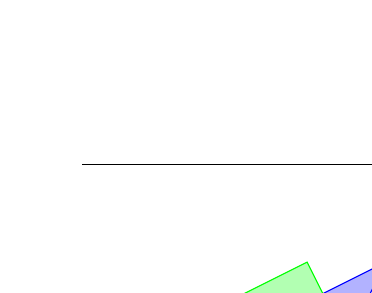
\begin{tikzpicture}
        \draw[color=blue,fill=blue!30] (1,0) -- (0.5,-1) -- (2.5,0) -- (3,1) -- cycle;
        \draw[color=green,fill=green!30] (1,0) -- (1.5,-1) -- (3.5,0) -- (3,1) -- cycle;
        \draw[color=red,fill=red!30] (0,0) -- (2,0) -- (4,1) -- (2,1) -- cycle;
        \draw[color=green,fill=green!30] (1,0) -- (0.5,1) -- (2.5,2) -- (3,1) -- cycle;
        \draw[color=blue,fill=blue!30] (1,0) -- (1.5,1) -- (3.5,2) -- (3,1) -- cycle;
    \end{tikzpicture}
    \begin{tikzpicture}
        \draw[color=blue,fill=blue!30] (0.5,-0.5) -- (1.5,0) -- (1.75,0.5) -- (0.75,0) -- cycle;
        \draw[color=green,fill=green!30] (1.75,0) -- (2.7913043055990334,0.5) -- (3.0151685536285298,0.07564192477122947) -- (2,-0.5) -- cycle;
        \draw[color=red,fill=red!30] (0,0) -- (1,0.5) -- (3.5,0.5) -- (2.5,0) -- cycle;
        \draw[color=blue,fill=blue!40] (0.75,0) -- (1.75,0.5) -- (2.25,1.5) -- (1.25,1) -- cycle;
        \draw[color=green,fill=green!30] (1,1.5) -- (1.75,0) -- (2.7913043055990334,0.5) -- (2,2) -- cycle;
        \draw[color=blue,fill=blue!30] (1.25,1) -- (2.25,1.5) -- (2.5,2) -- (1.5,1.5) -- cycle;
    \end{tikzpicture}
    \caption{五种不重合三平面关系}
\end{figure}

\subsubsection{点到平面的距离}
设$Ax+By+Cz+D=0$是一个平面,$\bm{n}=(A,B,C)$为其法向量,$P=(x_0,y_0,z_0)$为平面外一点,任取平面上一点$M(x,y,z)$,则点$P$到平面的距离为
\begin{equation}
    \label{eq:点到平面的距离公式}
    d = \abs{\overrightarrow{PM}\cdot\frac{\bm{n}}{\norm{\bm{n}}}}
    = \frac{\abs{A(x-x_0) + B(y-y_0) + C(z-z_0)}}{\sqrt{A^2+B^2+C^2}}
    = \frac{\abs{Ax_0+By_0+Cz_0+D}}{\sqrt{A^2+B^2+C^2}}
\end{equation}

\subsubsection{点到直线的距离}
设$\dfrac{x-x_0}{v_1} = \dfrac{y-y_0}{v_2} = \dfrac{z-z_0}{v_3}$是一条直线,$\bm{v}=(v_1,v_2,v_3)$,
点$P(x_1,y_1,z_1)$是直线外一点,$M$点坐标为$(x_0,y_0,z_0)$,利用平行四边形的面积可推出所求距离$d$为
\begin{marginfigure}
    \centering
    \begin{tikzpicture}
        \draw (-0.5, 0) -- (3.5, 0);
        \coordinate (M) at (0, 0);
        \coordinate (L) at (3, 0);
        \coordinate (P) at (1, 2);
        \coordinate (D) at (4, 2);
        \fill[blue!20!white] (M) -- (L) -- (D) -- (P) -- cycle;
        \draw[-stealth, thick] (M) -- (L);
        \draw[-stealth, thick] (M) -- (P);
        \draw (L) -- (4, 2)  -- (P) -- (1, 0) node [pos=0.5,right] {$d$};
        \draw (1.2, 0) rectangle (1, 0.2);
        \node[below] at (M) {$M$};
        \node[below] at (L) {$\bm{v}$};
        \node[left] at (P) {$P$};
    \end{tikzpicture}
    \caption{点到直线的距离示意图}
\end{marginfigure}
\begin{equation}
    \label{eq:点到直线的距离公式}
    d = \frac{\norm{\overrightarrow{PM}\times\bm{v}}}{\norm{\bm{v}}}
\end{equation}

\subsubsection{异面直线间的距离}
设$L_1 : \bm{r} = \bm{r}_1 + t\bm{u},\, L_2 : \bm{r} = \bm{r}_2 + t\bm{v}$是两条异面直线,
则公垂线长度为
\begin{equation}
    \label{eq:异面直线间的距离公式}
    d
    = \abs{(\bm{r}_2 - \bm{r}_1)\cdot \frac{\bm{u}\times\bm{v}}{\norm{\bm{u}\times\bm{v}}}}
    = \frac{\abs{(\bm{r}_2 - \bm{r}_1, \bm{u}, \bm{v})}}{\norm{\bm{u}\times\bm{v}}}
\end{equation}
\begin{marginfigure}
    \centering
    \begin{tikzpicture}
        \coordinate (0) at (0, 0);
        \coordinate (1) at (0, 3);
        \coordinate (2) at (-1, 0.5);
        \coordinate (3) at (2, 2);
        \coordinate (4) at (3, -0.75);
        \coordinate (5) at (1.5, 1.75);
        \coordinate (6) at (2, -0.5);
        \coordinate (7) at (-1, -0.5);
        \coordinate (8) at (2, 1);
        \coordinate (9) at (1.5, 0.75);
        \coordinate (10) at (0, 1);
        \fill[blue!20!white] (7) -- (8) -- (3) -- (2) -- cycle;
        \fill[green!20!white] (0) -- (8) -- (4) --  cycle;
        \fill[red!40!white] (6) -- (5) -- (9) --  cycle;
        \draw[-stealth] (2) -- (3) node[right] {$\bm{v}$};
        \draw[-stealth] (0) -- (1) node[above] {$\bm{u}\times\bm{v}$};
        \draw[-stealth] (0) -- (4) node[right] {$\bm{u}$};
        \draw[-stealth] (6) -- (5) node[pos=0.5,right] {$\bm{r}_2-\bm{r}_1$};
        \draw[red,very thick] (0) -- (10) node[pos=0.5, left, black] {$d$};
    \end{tikzpicture}
    \caption{异面直线间的距离示意图}
\end{marginfigure}

\section{曲线与曲面}
\subsection{空间曲面}
\subsubsection{曲面方程}
空间曲面常用显式方程$z=f(x,y)$,隐式方程$F(x,y,z)=0$,向量方程$\bm{r} = \bm{r}(u,v)$
和参数方程$x=x(u,v),y=y(u,v),z=z(u,v)$。

曲面显式方程$z=f(x,y)$是按照\textcolor{red}{投影}方式建立的空间曲面到平面区域的一一对应。

曲面的向量方程$\bm{r} = \bm{r}(u,v)$或参数方程$x=x(u,v),y=y(u,v),z=z(u,v)$是按照\textcolor{red}{变换}建立的空间曲面到平面区域的一一对应。

隐式方程$F(x,y,z)=0$是三元函数的零截面,常常需要化为参数方程或分片化为参数方程或局部地向切平面作投影进行处理。

\subsubsection{柱面}
给定一空间曲线$C$和直线$L$,过曲线$C$上任意一点,且与直线$L$平行的全体直线构成一个空间的曲面$\Sigma$,称这个曲面为\textcolor{red}{\textbf{\textsf{柱面}}}。
曲线$C$称为柱面的\textcolor{red}{\textbf{\textsf{准线}}},直线$L$称为柱面的\textcolor{red}{\textbf{\textsf{母线}}}。柱面的表示为
\begin{equation}
    \label{eq:柱面方程}
    \Sigma : \bm{r} = \bm{r}(t,s) = \bm{r}_0(t) + s\bm{v}
\end{equation}
其中$\bm{r}_0(t)$为母线上的点,$\bm{v}$为准线的方向向量。

\subsubsection{锥面}
给定一空间曲线$C$和一固定点$P$,曲线$C$上任意一点与点$P$构成的直线全体构成的曲面$\Sigma$,称为\textcolor{red}{\textbf{\textsf{锥面}}}。
曲线$C$称为锥面的\textcolor{red}{\textbf{\textsf{准线}}},过曲线$C$上任意一点和点$P$的直线称为锥面的\textcolor{red}{\textbf{\textsf{母线}}}。
\begin{equation}
    \label{eq:锥面方程}
    \Sigma : \bm{r} = \bm{r}(t,s) = (1-s)\bm{r}_0(t) + s\bm{v}
\end{equation}
其中$\bm{r}_0(t)$为母线上的点,$\bm{v}$为准线的方向向量。

\subsubsection{旋转面}
如果一条空间曲线$C$绕一固定直线$L$的旋转图形为一曲面,则称该曲面为旋转面。$L$为旋转轴,$C$称为旋转面的母线。

当旋转轴为$x,y,z$其中之一时,这种曲线变曲面的特征是\textcolor{red}{\textbf{\textsf{非轴变量变开方}}}。
例如平面曲线$L:f(y,z)=0$绕$z$轴的旋转面为
\[ f(\pm\sqrt{x^2+y^2}, z) = 0 \]
例如平面曲线$L:f(y,z)=0$绕$y$轴的旋转面为
\[ f(y, \pm\sqrt{x^2+z^2}) = 0 \]

\subsection{空间曲线}
\subsubsection{曲线方程}
空间曲线常用交面式方程$\displaystyle\begin{cases}
        f(x,y,z)=0 \\
        g(x,y,z)=0
    \end{cases}$,向量方程$\bm{r} = \bm{r}(t)$和参数方程$x=x(t),y=y(t),z=z(t)$表示。

\subsubsection{曲线的投影}
设曲线
\[
    C:
    \begin{cases}
        f(x,y,z)=0 \\
        g(x,y,z)=0
    \end{cases}
\]
是一条空间曲线方程,如果从上述方程中消取$z$,则会得到一个柱面方程,记作$H(x,y)=0$,该柱面的母线平行于$z$轴,
准线为$C$,习惯上称为$C$的\textcolor{red}{\textbf{\textsf{投影柱面}}},并称平面曲线
\[
    \begin{cases}
        H(x,y)=0 \\
        z=0
    \end{cases}
\]
为$C$的\textcolor{red}{\textbf{\textsf{消$z$投影曲线}}}。类似地有,消$x$投影曲线,消$y$投影曲线。

\textbf{消去变量定投影}的方法在多元函数的积分计算中非常有用,是多重积分和线面积分转化为定积分的重要工具。

\subsubsection{切向量的计算}
设$\bm{r}=(x(t),y(y),z(t))$是一条空间曲线,如果$x(t),y(y),z(t)$都是连续函数,
则称该曲线为\textcolor{red}{\textbf{\textsf{连续曲线}}}。如果$x(t),y(y),z(t)$均可导,且导函数连续,
则称该曲线为\textcolor{red}{\textbf{\textsf{光滑曲线}}}。

对于曲线的切向量计算如下
\begin{equation}
    \dv{\bm{r}}{t}
    = \lim_{\Delta t \to 0}\frac{\Delta \bm{r}}{\Delta t}
    = \lim_{\Delta t \to 0}\frac{\bm{r}(t+\Delta t) - \bm{r}(t)}{\Delta t}
    = (x'(t),y'(t),z'(t))
\end{equation}
则有微分
\begin{equation}
    \dd{\bm{r}} = (\dd{x}, \dd{y}, \dd{z})
\end{equation}
特别的有
\begin{equation}
    \dd{s} = \norm{\dd{\bm{r}}} = \sqrt{\dd{x^2}+ \dd{y^2} + \dd{z^2}}
\end{equation}

\subsubsection{曲面的法线量}
对于一元函数$f(x)$,其点$(x_0,f(x_0))$处的切向量为$(1,f'(x_0))$,法向量为$(f'(x_0),-1)$。
对于二元函数$z=f(x,y)$上的任意一点$(x_0,y_0,f(x_0,y_0))$,其法向量为$(z_x',z_y',-1)$。
\begin{marginfigure}
    \centering
    \begin{tikzpicture}
        \draw[color=red] (1,2) -- (2,2) -- (2,4) -- cycle;
        \draw[color=red] (1,2) -- (3,2) -- (3,1) -- cycle;
        \draw[color=black] (1,2) arc (153.43:120:2.24) node[pos=1.1,right]{$f(x)$};
        \draw[color=black] (1,2) arc (153.43:170:2.24);
        \node[left] (A) at (1,2) {$A$};
        \node[above right] (B) at (2,2) {$B$};
        \node[right] (C) at (2,4) {$C$};
        \node[right] (E) at (3,2) {$E$};
        \node[right] (F) at (3,1) {$F$};
    \end{tikzpicture}
\end{marginfigure}

\begin{proof}
    \begin{enumerate}[(1)]
        \item 一元函数$f(x)$的证明如下图,其中$AC$为切线,$\abs{AB}=1$,则$\abs{CB}=f'(x)$,那么得出向量
              $\overrightarrow{AC}=(1,f'(x))$,同时令$\abs{EF}=1$根据$\triangle ABC \cong\triangle FEB$,
              那么$\abs{AE}=f'(x)$,所以法向量$\overrightarrow{AF}=(f'(x),-1)$

        \item 设二元函数$z=f(x,y)$上的任意一点的法向量为$\bm{n}$,则$\bm{n}$在平面$xOz, yOz$的投影向量分别为,
              $(z_x',-1),(z_y',-1)$,因此$\bm{n} = (z_x',z_y',-1)$
    \end{enumerate}
\end{proof}

\subsection{二次曲面}
由三元二次方程所确定的曲面称为二次曲面。二次曲面与平面的交线都是二次曲线。

\subsubsection{椭球面}
由方程
\begin{equation}
    \frac{x^2}{a^2} + \frac{y^2}{b^2} + \frac{z^2}{c^2} = 1
\end{equation}
所确定的曲面称为椭球面。任意平面与椭球的交线均为椭圆。
\begin{marginfigure}
    \centering
    \begin{tikzpicture}
        \begin{axis}[hide axis,colormap/cool,z buffer=sort, opacity=0.5, axis equal]
            \addplot3[surf, domain=0:360,y domain=0:180] ({1.5*cos(x)*sin(y)},{sin(x)*sin(y)},{cos(y)});
        \end{axis}
    \end{tikzpicture}
    \caption{椭球面。}
\end{marginfigure}

\subsubsection{单叶双曲面}
分别由方程
\begin{align}
    \frac{x^2}{a^2} + \frac{y^2}{b^2} - \frac{z^2}{c^2}   & = 1 \\
    \frac{x^2}{a^2} - \frac{y^2}{b^2} + \frac{z^2}{c^2}   & = 1 \\
    - \frac{x^2}{a^2} + \frac{y^2}{b^2} + \frac{z^2}{c^2} & = 1
\end{align}
所确定的曲面称为单叶双曲面。
\begin{marginfigure}
    \centering
    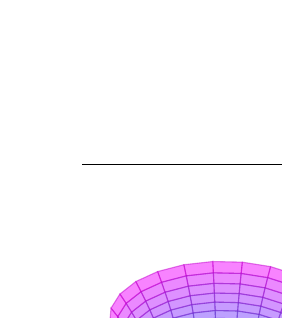
\begin{tikzpicture}
        \begin{axis}[hide axis,colormap/cool,z buffer=sort, opacity=0.5, axis equal]
            \addplot3[surf, domain=0:360,y domain=-1:1] ({cosh(y)*cos(x)},{cosh(y)*sin(x)},{sinh(y)});
        \end{axis}
    \end{tikzpicture}
    \caption{单叶双曲面。}
\end{marginfigure}

\subsubsection{二次锥面}
分别由方程
\begin{align}
    \frac{x^2}{a^2} + \frac{y^2}{b^2} - \frac{z^2}{c^2}   & = 0 \\
    \frac{x^2}{a^2} - \frac{y^2}{b^2} + \frac{z^2}{c^2}   & = 0 \\
    - \frac{x^2}{a^2} + \frac{y^2}{b^2} + \frac{z^2}{c^2} & = 0
\end{align}
所确定的曲面称为二次锥面。
\begin{marginfigure}
    \centering
    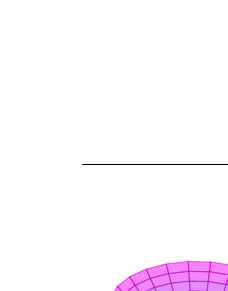
\begin{tikzpicture}
        \begin{axis}[hide axis,colormap/cool,z buffer=sort, opacity=0.5, axis equal]
            \addplot3[surf, domain=0:360,y domain=-1:1] ({y*cos(x)},{y*sin(x)},{y});
        \end{axis}
    \end{tikzpicture}
    \caption{二次锥面。}
\end{marginfigure}

\subsubsection{双叶双曲线}
分别由方程$(pq>0)$
\begin{align}
    \frac{x^2}{a^2} + \frac{y^2}{b^2} - \frac{z^2}{c^2}   & = -1 \\
    \frac{x^2}{a^2} - \frac{y^2}{b^2} + \frac{z^2}{c^2}   & = -1 \\
    - \frac{x^2}{a^2} + \frac{y^2}{b^2} + \frac{z^2}{c^2} & = -1
\end{align}
所确定的曲面称为双叶双曲线。
\begin{marginfigure}
    \centering
    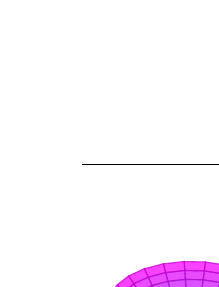
\begin{tikzpicture}
        \begin{axis}[hide axis,colormap/cool,z buffer=sort, opacity=0.5, axis equal]
            \addplot3[surf, domain=0:360,y domain=-3:3] ({y*cos(x)},{y*sin(x)},{sqrt(y^2+1)});
            \addplot3[surf, domain=0:360,y domain=-3:3] ({y*cos(x)},{y*sin(x)},{-sqrt(y^2+1)});
        \end{axis}
    \end{tikzpicture}
    \caption{双叶双曲线。}
\end{marginfigure}

\subsubsection{双曲抛物面}
分别由方程
\begin{align}
    z = -\frac{x^2}{2p} + \frac{y^2}{2q} \\
    x = -\frac{y^2}{2p} + \frac{z^2}{2q} \\
    y = -\frac{z^2}{2p} + \frac{x^2}{2q}
\end{align}
所确定的曲面称为双曲抛物面。
\begin{marginfigure}
    \centering
    \begin{tikzpicture}
        \begin{axis}[hide axis,colormap/cool,z buffer=sort, opacity=0.5, axis equal,view/h=60]
            \addplot3[surf] {0.2*(-x^2+y^2)};
        \end{axis}
    \end{tikzpicture}
    \caption{双曲抛物面。}
\end{marginfigure}

\subsubsection{椭圆抛物面}
分别由方程
\begin{align}
    z = \frac{x^2}{2p} + \frac{y^2}{2q} \\
    x = \frac{y^2}{2p} + \frac{z^2}{2q} \\
    y = \frac{z^2}{2p} + \frac{x^2}{2q}
\end{align}
所确定的曲面称为椭圆抛物面。
\begin{marginfigure}
    \centering
    \begin{tikzpicture}
        \begin{axis}[hide axis,colormap/cool,z buffer=sort, opacity=0.5, axis equal]
            \addplot3[surf] {0.2*(x^2+y^2)};
        \end{axis}
    \end{tikzpicture}
    \caption{椭圆抛物面。}
\end{marginfigure}

对于截面曲线的判断,只需要让其中一个分量等于零,在根据平面曲线来判断曲线的 类型。
% \part{附录}

\section{常用不等式}
\subsection{三角不等式}
\begin{align}
    \label{eq:三角不等式}
    \abs{x-y}     & \leq \abs{x-z} + \abs{z-y} \\
    \abs{x \pm y} & \leq \abs{x} + \abs{y}
\end{align}


\subsection{平均不等式}
从左到右为调和平均数、几何平均数、算术平均数
\begin{equation}
    \label{eq:平均不等式}
    \frac{n}{\frac{1}{x_1} + \frac{1}{x_2} + \cdots + \frac{1}{x_n}}
    \leq \sqrt[n]{x_1x_2 \cdots x_n}
    \leq \frac{x_1 + x_2 + \cdots x_n}{n}
\end{equation}
当且仅当$ x_1 = x_2 = \cdots = x_n $时,等号成立。

\subsection{面积不等式}
\begin{alignat}{1}
    \label{eq:面积不等式1} \sin x         <  x         < \tan x & \qquad (0<x<\frac{\pi}{2}) \\
    \label{eq:面积不等式2} \frac{x}{1+x}  <  \ln(1+x)  < x      & \qquad (x > -1, x \neq 0)
\end{alignat}
\begin{marginfigure}
    \centering
    \begin{tikzpicture}[scale=2.5,domain=0:1.2]
        \coordinate[label=below left:{\scriptsize$O$}]  (O) at (0, 0);
        \coordinate[label=below:{\scriptsize$\mat{A}$}]       (A) at (1, 0);
        \coordinate[label=left:{\scriptsize$B$}]        (B) at ({cos(30)}, {sin{30}});
        \coordinate[label=below right:{\scriptsize$C$}] (C) at (1, {tan(30)});

        \fill[green!20!white] (A) -- (O) -- (B) -- cycle;
        \fill[red]            (A) arc (0:30:1) -- cycle;
        \fill[blue!30!white]  (A) arc (0:30:1) -- (C) -- cycle;
        \draw (A) arc (0:90:1);
        \draw plot (\x, {tan(30)*\x});
        \draw (A) -- (C);
        \draw[->] (-0.1, 0) -- (1.3, 0) node[right] {$x$};
        \draw[->] (0, -0.1) -- (0, 1.3) node[above] {$y$};
    \end{tikzpicture}
    \caption{面积不等式\ref{eq:面积不等式1},单位圆}
    \label{fig:面积不等式1}
\end{marginfigure}
\begin{proof}
    对于不等式\ref{eq:面积不等式1},当$0<x<\frac{\pi}{2}$时,由图\ref{fig:面积不等式1}可知,$S_{\triangle AOB} < S_{\text{扇形}AOB} < S_{\triangle AOC}$,对应的值为
    \[ \frac{1}{2}\sin x < \frac{1}{2}x < \frac{1}{2}\tan x \]
\end{proof}

\begin{proof}
    对于不等式\ref{eq:面积不等式2},由\ref{fig:面积不等式2}可知,$S_{ABDC} < S_{ABDE}< S_{ABFE}$,即
    \[ \frac{x}{1+x}<\ln (1+x) < x \]
\end{proof}
\begin{marginfigure}
    \centering
    \begin{tikzpicture}[scale=0.8, declare function={f(\x)=1/\x;}]
        \coordinate[label=below left:{\scriptsize$O$}]   (O) at (0, 0);
        \coordinate[label=below:{\scriptsize$A(1,0)$}]   (A) at (1, 0);
        \coordinate[label=below:{\scriptsize$B(1+x,0)$}] (B) at (3, 0);
        \coordinate[label=above left:{\scriptsize$C$}]   (C) at (1, {f(3)});
        \coordinate[label=above right:{\scriptsize$D$}]  (D) at ({3}, {f(3)});
        \coordinate[label=left:{\scriptsize$E$}]         (E) at (1, {f(1)});
        \coordinate[label=right:{\scriptsize$F$}]        (F) at ({3}, {f(1)});

        \fill[green!20!white] (A) -- (B) -- (D) -- (C) -- cycle;
        \fill[red]            (C) -- (E) -- plot[domain=1:{3}](\x, {f(\x)}) -- cycle;
        \fill[blue!30!white]  (E) -- plot[domain=1:{3}](\x, {f(\x)}) -- (F) -- cycle;

        \draw[domain=3.8:0.3] plot (\x, {f(\x)}) node[right] {\scriptsize$f(x)=\frac{1}{x}$};
        \draw[->] (-0.1, 0) -- (4, 0)          node[right] {$x$};
        \draw[->] (0, -0.1) -- (0, 4)          node[above] {$y$};
    \end{tikzpicture}
    \caption{面积不等式\ref{eq:面积不等式2}}
    \label{fig:面积不等式2}
\end{marginfigure}

\subsection{压缩不等式}
\begin{align}
    \label{eq:压缩不等式sin} \abs{\sin x - \sin y} & \leq \abs{x - y} \\
    \label{eq:压缩不等式cos} \abs{\cos x - \cos y} & \leq \abs{x - y}
\end{align}

\subsection{阶乘不等式}
\begin{align}
    \label{eq:阶乘不等式1} 2^n < n! \leq (\frac{n+1}{2})^n & \qquad (n>4) \\
    \label{eq:阶乘不等式2} n! \geq n^{n/2}                 &
\end{align}
\begin{proof}
    不等式\ref{eq:阶乘不等式1}左侧,当$n>4$时,后续乘法$n!$总是大于$2^n$。对于右侧得不等式,根据平均不等式\ref{eq:平均不等式},
    \[ \sqrt[n]{n!} \leq \frac{1+2+\cdots+n}{n} = \frac{1+n}{2} \]
    由此可知当$n>1$时,$n! < (\frac{n+1}{2})^n$
\end{proof}
\begin{proof}
    对于不等式\ref{eq:阶乘不等式2},只需证明$\sqrt[n]{n!} \geq \sqrt{n}$,联想到平均不等式\ref{eq:平均不等式},只证明要下述不等式即可
    \[ \sqrt[n]{n!} \geq \frac{n}{1 + \frac{1}{2} + \cdots + \frac{1}{n}} \geq \sqrt{n} \]
    即
    \[ \sqrt{n} = \frac{n}{\sqrt{n}} > 1 + \frac{1}{2} + \cdots + \frac{1}{n} \]

    令$x_n=1+\frac{1}{2}+\frac{1}{3}+\cdots+\frac{1}{n}-\sqrt{n}$,则有$x_5 < 0$,并在$n>3$时有
    \begin{alignat*}{1}
        x_{n+1}-x_{n} & =    \frac{1}{n+1} + \sqrt{n} - \sqrt{n-1}  =  \frac{1}{n+1} - \frac{1}{\sqrt{n} + \sqrt{n+1}} \\
                      & \leq \frac{1}{n+1} - \frac{1}{2\sqrt{n+1}} = \frac{2 - \sqrt{n+1}}{2(n+1)} < 0
    \end{alignat*}
    所以在$n \geq 5$时,$x_n < 0$,因而有
    \[ \sqrt[n]{n!} \geq \frac{n}{1 + \frac{1}{2} + \cdots + \frac{1}{n}} > \frac{n}{\sqrt{n}} = \sqrt{n} \]
    而对于$n<5$,直接验证不等式\ref{eq:阶乘不等式2}即可。
\end{proof}

\subsection{夹挤不等式}
\begin{alignat}{2}
    \label{eq:夹挤不等式1} 2(\sqrt{n+1}-\sqrt{n}) & < \frac{1}{\sqrt{n}} & < 2(\sqrt{n}-\sqrt{n-1}) \\
    \label{eq:夹挤不等式2} \ln( 1+\frac{1}{n} )   & < \frac{1}{n}        & < \ln(1 + \frac{1}{n-1})
\end{alignat}

\subsection{柯西不等式}
\begin{align}
    \label{eq:柯西不等式}
    \left(\int_a^b f(x)g(x)\dd{x} \right)^2 & \leq \left( \int_a^bf^2(x)\dd{x} \right) \left( \int_a^bg^2(x)\dd{x} \right) & \text{积分形式}
\end{align}

\subsection{闵可夫斯基不等式}
\begin{align}
    \label{eq:闵可夫斯基不等式}
    \left( \int_a^b[f(x)+g(x)]^2\dd{x} \right)^{1/2}
    \leq
    \left( \int_a^bf^2(x)\dd{x} \right)^{1/2} +\left( \int_a^bg^2(x)\dd{x} \right)^{1/2}
\end{align}

\section{导数表}
\subsection{指数函数、对数函数}
\begin{multicols}{2}
    \begin{enumerate}
        \item $(x^\alpha)' = \alpha x^{\alpha-1}$
        \item $(a^x)' = a^x\ln a \qquad (a>0, a\neq 1)$
        \item $(\log_a x)' = \frac{1}{x\ln a} \qquad(a>0,a\neq 1)$
    \end{enumerate}
\end{multicols}

\subsection{三角函数、反三角函数}
\begin{multicols}{2}
    \begin{enumerate}
        \item $(\tan x)' =  \sec^2 x =  \frac{1}{\cos^2 x}$
        \item $(\cot x)' = -\csc^2 x = -\frac{1}{\sin^2 x}$
        \item $(\sec x)' =  \tan x\sec x$
        \item $(\csc x)' = -\cot x\csc x$
        \item $(\arcsin x)' = \frac{1}{\sqrt{1-x^2}} \qquad (\abs{x} < 1)$
        \item $(\arccos x)' =-\frac{1}{\sqrt{1-x^2}} \qquad (\abs{x} < 1)$
        \item $(\arctan x)' = \frac{1}{1+x^2}$
        \item $(\arccot x)' =-\frac{1}{1+x^2}$
    \end{enumerate}
\end{multicols}

\subsection{双曲函数、反双曲函数}
\begin{enumerate}
    \item $(\sinh x)' = \cosh x$
    \item $(\cosh x)' = \sinh x$
    \item $(\tanh x)' = \frac{1}{\cosh^2 x}$
\end{enumerate}
\begin{enumerate}[\textcolor{red}{$\bigstar$}]
    \item $(\sinh^{-1} x)' = (\ln (x+\sqrt{x^2 + 1}))' = \frac{1}{\sqrt{x^2 + 1}}$
    \item $(\cosh^{-1} x)' = (\ln (x+\sqrt{x^2 - 1}))' = \frac{1}{\sqrt{x^2 - 1}} \qquad (\abs{x} > 1)$
    \item $(\tanh^{-1} x)' = (\frac{1}{2}\ln \frac{1+x}{1-x})' = \frac{1}{1-x^2} \qquad (\abs{x} < 1)$
\end{enumerate}

\subsection{部分高阶导数}
\begin{enumerate}
    \item $(a^x)^{(n)} = a^x\ln^n a$
    \item $(\sin kx)^{(n)} = k^n \sin(kx+n\cdot \frac{\pi}{2})$ (导一次,加半$\pi$)
    \item $(\cos kx)^{(n)} = k^n \cos(kx+n\cdot \frac{\pi}{2})$ (导一次,加半$\pi$)
\end{enumerate}

\section{常用泰勒展开}
以下泰勒展开中$(x\to 0)$
\begin{enumerate}
    \item $\mathrm{e}^x = 1 + x + \dfrac{x^2}{2!} + \cdots + \dfrac{x^n}{n} + o(x^n)$
    \item $\ln(1+x) = x - \dfrac{1}{2}x^2 + \dfrac{1}{3}x^3 -\cdots+(-1)^{n+1}\dfrac{1}{n}x^n + o(x^n)$
    \item $\sin x = x-\dfrac{x^3}{3!} + \dfrac{x^5}{5!} -\cdots +(-1)^{n+1}\dfrac{x^{2n-1}}{(2n-1)!}+o(x^{2n-1})$
    \item $\cos x = 1 - \dfrac{x^2}{2!} + \dfrac{x^4}{4!} - \cdots + (-1)^n\dfrac{x^{2n}}{(2n)!} + o(x^{2n})$
    \item $\arctan x = x - \dfrac{x^3}{3} + \cdots +(-1)^{n+1}\dfrac{x^{2n-1}}{2n-1}+o(x^{2n-1})$
    \item $(1+x)^\alpha = 1 + \alpha x +\dfrac{\alpha(\alpha-1)}{2!}x^2 + \dfrac{\alpha(\alpha-1)(\alpha-2)}{3!}x^3 + o(x^3)$
    \item $\tan x = x + \dfrac{1}{3}x^3 + \dfrac{2}{15}x^5 + o(x^5)$
\end{enumerate}

\section{常微分方程解法总结}
\begin{fullpage}
    \begin{tabularx}{\textwidth}{@{}XXX@{}}
        \toprule
        \multicolumn{1}{c}{微分方程}                                                                   & \multicolumn{1}{c}{解法}                                             & \multicolumn{1}{c}{通解}                                                           \\
        \midrule
        \rowcolor{gray!40}
        \multicolumn{3}{c}{可分离方程}                                                                                                                                                                                                                             \\
        一阶,变量$x$和$y$均可分离(一般情况, 下面有特殊情况)\[P_1(x)Q_1(y)+P_2(x)Q_2(y)\dv{y}{x}=0\] & 分离变量(除以$P_2Q_1$)                                             & \[ \int^x \frac{P_1(t)}{P_2(t)}\dd{t} + \int^y\frac{Q_2(t)}{Q_1(t)}\dd{t} = C \]   \\
        \midrule
        一阶,变量$x$可分离 \[\dv{y}{x}=F(x)\]                                                         & 直接积分                                                             & \[ y=\int^x F(t)\dd{t} + C \]                                                      \\
        \midrule
        一阶自治,变量$y$可分离 \[ \dv{y}{x}=F(y) \]                                                   & 分离变量(除以$F$)                                                  & \[ x=\int^y \frac{\dd{t}}{F(t)} + C \]                                             \\
        \midrule
        一阶,变量$x$和$y$均可分离 \[ P(y)\dv{y}{x} + Q(x) = 0 \]                                      & 整个积分                                                             & \[ \int^y P(t)\dd{t} + \int^x Q(t)\dd{t} = C \]                                    \\
        \midrule
        \rowcolor{gray!40}
        \multicolumn{3}{c}{一般一阶微分方程}                                                                                                                                                                                                                       \\
        一阶,齐次 \[ \dv{y}{x} = F\left(\frac{y}{x}\right) \]                                         & 令$y=ux$,然后通过分离变量$u$和$x$求解                               & \[ \ln(Cx) = \int^{\frac{y}{x}} \frac{\dd{t}}{F(t)-t} \]                           \\
        \midrule
        一阶,可分离变量 \[ y=M(xy) + xN(xy)\dv{y}{x} = 0 \]                                           & 根据$\dd{\ln(xy)}=\frac{\dd{x}}{x} + \frac{\dd{y}}{y}$,方程除以$xy$ & \[ \ln(Cx) = \int^{xy} = \frac{N(t)\dd{t}}{t[N(t)-M(t)]} \]如果$N=M$,则解为$xy=C$ \\
        \midrule
        恰当微分,一阶 \[ M(x,y)\dv{y}{x} + N(x,y) = 0 \] 其中$\displaystyle \pdv{M}{x}=\pdv{N}{y}$    & 整个积分                                                             &
        {\[\begin{split}F(x,y) = & \int^y M(x,t)\dd{t} + \int^x N(t,y)\dd{t} \\& + Y(y) +X(x) = C\end{split}\]} 其中$Y(y)$和$X(x)$时积分处理的函数而不是常数,将他们列在这里以使最终函数$F(x,y)$满足初始条件                                                                                                                              \\
        \bottomrule
    \end{tabularx}
\end{fullpage}

\begin{fullpage}
    \begin{tabularx}{\textwidth}{@{}XXX@{}}
        \toprule
        \multicolumn{1}{c}{微分方程}                                                                   & \multicolumn{1}{c}{解法}                                                                                                                                                   & \multicolumn{1}{c}{通解}                                             \\
        \midrule
        \rowcolor{gray!40}
        \multicolumn{3}{c}{一般一阶微分方程}                                                                                                                                                                                                                                                                                                               \\
        反常微分, 一阶 \[ M(x,y)\dv{y}{x} + N(x,y) = 0 \] 其中$\displaystyle \pdv{M}{x}\neq\pdv{N}{y}$ & 积分变量$\mu(x,y)$ 满足\[\pdv{(\mu M)}{x}=\pdv{(\mu N)}{y}\]                                                                                                               & 如果可以得到$\mu(x,y)$
        {\[\begin{split}F(x,y) = & \int^y \mu(x,t)M(x,t)\dd{t} \\ &+ \int^x \mu(t,y)N(t,y)\dd{t} \\& + Y(y) +X(x) = C\end{split}\]}                                                                                                                                                                                                                                                                                                                   \\
        \midrule
        \rowcolor{gray!40}
        \multicolumn{3}{c}{一般二阶微分方程}                                                                                                                                                                                                                                                                                                               \\
        二阶, 自治\[ \dv[2]{y}{x} = F(y) \]                                                            & 原方程乘以$\displaystyle 2\dv{y}{x}$,代换$2\dv{y}{x}\dv[2]{y}{x} = \dv{x}(\dv{y}{x})^2$然后两次积分                                                                       & \[ x=\pm\int^y \frac{\dd{t}}{\sqrt{2\int^t F(m)\dd{m}} +C_1} +C_2 \] \\
        \midrule
        \rowcolor{gray!40}
        \multicolumn{3}{c}{线性方程}                                                                                                                                                                                                                                                                                                                       \\
        一阶线性,非齐次的函数系数\[ \dv{y}{x + P(x)y = Q(x)} \]                                       & 积分因子$\mathrm{e}^{\int^x P(t)\dd{t}}$                                                                                                                                   &
        \[\begin{split} y = \mathrm{e}^{-\int^x P(s)\dd{s}}\left[\int^x \mathrm{e}^{\int^t P(m)\dd{m}}Q(t)\dd{t}\right.\\ + \left.C \vphantom{\int^x}\right]\end{split} \]                                                                                                                                                                                                                                                                                                                    \\
        \midrule
        二阶线性,非齐次的常系数\[ \dv[2]{y}{x}+b\dv{y}{x} + cy = r(x) \]                              & 设$y_c=\mathrm{e}^{\alpha x}$代换并解出$\alpha$中的多项式,求出线性无关函数$\mathrm{e}^{\alpha_j x}$,特解$y_p$一般运用常数变易法, 虽然对于非常容易的$r(x)$可以直观判断。 &                                                                      \\
        \bottomrule
    \end{tabularx}
\end{fullpage}

\section{线性代数相关公式}
\subsection{伴随矩阵的公式}\label{sec:伴随矩阵的公式}

设$\mat{A}$为$n$阶矩阵
\begin{enumerate}[(1)]
    \item $\mat{A}\mat{A}^*=\mat{A}^*\mat{A}=|\mat{A}|\mat{E}$;
    \item $(k\mat{A})^* = k^{n-1}\mat{A}^*$;
    \item $(\mat{A}^*)^\intercal = (\mat{A}^\intercal)^*$;
    \item $|\mat{A}^*|=|\mat{A}|^{n-1}$;
    \item $(\mat{A}^*)^*=|\mat{A}|^{n-2}A$;
    \item $(\mat{A}^*)^{-1} = (\mat{A}^{-1})^* = \dfrac{1}{|\mat{A}|}\mat{A}$;
    \item $
              r(\mat{A}^*) =
              \begin{cases}
                  n, & r(\mat{A})=n,   \\
                  1, & r(\mat{A})=n-1, \\
                  0, & r(\mat{A})<n-1.
              \end{cases}
          $
\end{enumerate}

\subsection{矩阵的秩相关公式}
\label{sec:矩阵的秩相关公式}

\begin{enumerate}[(1)]
    \item $r(\mat{A}^\intercal) = r(\mat{A})$;
    \item $r(k\mat{A}) = r(\mat{A}), k\neq 0$;
    \item $r(0\mat{E} - \mat{A}) = r(\mat{A})$;
    \item $r(\mat{A}-\mat{E}) = r(\mat{E}-\mat{A})$;
    \item $r(\mat{A}+\mat{B})\leq r(\mat{A}) + r(\mat{B})$;
    \item $r(\mat{AB})\leq \min(r(\mat{A}),r(\mat{B}))$;
    \item 若$\mat{A}$可逆,则$r(\mat{AB})=r(\mat{BA})=r(\mat{B})$;
    \item $r(\mat{A}^\intercal\mat{A}) = r(\mat{A})$利用$\mat{AX}=\bm{0},\mat{A}\mat{A}^\intercal\mat{X}=\bm{0}$同解秩相等;
    \item 西尔维斯特不等式\label{eq:西尔维斯特不等式}:$\mat{A}_{m\times n}, \mat{B}_{n\times s}$,则$r(\mat{A})+r(\mat{B})-n\leq r(\mat{AB})$;
    \item $
              r\begin{pmatrix}
                  \mat{A} & \mat{0} \\
                  \mat{0} & \mat{B}
              \end{pmatrix}
              =r(\mat{A})+r(\mat{B})
          $
    \item $\mat{A}\sim \mat{B}$,则$r(\mat{A})=r(\mat{B}), r(\mat{A}+k\mat{E})=r(\mat{B}+k\mat{E})$
\end{enumerate}

\subsection{可逆矩阵的性质}\label{sec:可逆矩阵的性质}
设矩阵$\mat{A},\mat{B}$可逆,$k=\neq 0$,则有如下性质
\begin{enumerate}[(1)]
    \item $\mat{A}^{-1}$可逆,$(\mat{A}^{-1})^{-1} = \mat{A}$;
    \item $k\mat{A}$可逆,$(k\mat{A}^{-1}) = \frac{1}{k} \mat{A}^{-1}$;
    \item $\mat{AB}$可逆,$(\mat{AB})^{-1} = \mat{A}^{-1}\mat{B}^{-1}$;
    \item $\mat{A}^\intercal$可逆,$(\mat{A}^\intercal)^{-1} = (\mat{A}^{-1})^\intercal$。
\end{enumerate}
\end{document}